\documentclass[12pt, a4paper]{article}

% --- layout -----------------------------------------------------------------
\usepackage{geometry}
\usepackage{float}
\usepackage{algorithm}       % after float: both patch the float mechanism
\usepackage{algpseudocode}
\usepackage{afterpage}
\usepackage{pdfpages}
\setlength{\emergencystretch}{2em}
\usepackage{hyphenat}

% --- encoding and symbols ---------------------------------------------------
\usepackage[utf8]{inputenc}
\usepackage{textgreek}
\usepackage{amsmath}
\usepackage{amssymb}

% --- figures ----------------------------------------------------------------
\usepackage{tikz}
\usetikzlibrary{arrows.meta, fit, positioning}

% --- tables -----------------------------------------------------------------
\usepackage{booktabs}
\usepackage{array}
\usepackage{tabularx}
\usepackage{longtable}
\newcolumntype{L}[1]{>{\raggedright\arraybackslash}p{#1}}

% --- references and acronyms ------------------------------------------------
\usepackage{caption}
\usepackage{xurl}           % long bibliography URLs break across lines
\usepackage{hyperref}
\usepackage[printonlyused]{acronym}

% --- float notes and pseudocode conventions ---------------------------------
% Every table and figure carries a short title in \caption and a self-contained
% note in \tabnote directly beneath it, so a float can be read without the body.
% In a longtable the note goes in a \multicolumn row instead.
\newcommand{\tabnote}[1]{\par\vspace{2pt}\noindent\begin{minipage}{\linewidth}\footnotesize\sloppy #1\end{minipage}\par\vspace{4pt}}
\usepackage{etoolbox}
\AtBeginEnvironment{algorithmic}{\small}   % compact, as in the reference paper
\algrenewcommand\alglinenumber[1]{}
\captionsetup[algorithm]{labelsep=space}

% NOTE (template): class, geometry and the title page below are provisional.
% Confirm the UCT / departmental mini-dissertation specification and adjust.
% Everything else in this document is template-agnostic.

\title{Buy Now, Pay Later and Household Credit Distress \\ in South Africa: An Agent-Based Model}
\author{Marc Levin \\[0.5em]
    University of Cape Town \\
    Cape Town, South Africa \\[0.3em]
    \texttt{LVNMAR013@myuct.ac.za}}
\date{\today}

\begin{document}

\maketitle

% ============================================================================
% FRONT MATTER
% ============================================================================

\section*{Declaration}
\addcontentsline{toc}{section}{Declaration}

% TODO (front matter): replace with the wording required by the UCT declaration
% and plagiarism form. Blocked on the departmental template.

\noindent I know the meaning of plagiarism and declare that all the work in this
document, save for that which is properly acknowledged, is my own. This work has
not been submitted for any other degree or examination at any other university.

\vspace{2em}
\noindent Signed: \hrulefill \qquad Date: \hrulefill

\section*{Abstract}
\addcontentsline{toc}{section}{Abstract}

% Every number is read from a generated table or results/summary/results_numbers.json:
% 14.2% from tab:ccmr; 37% and 52% from Section 4.2 (stack_holders_loyal_beta0, tab:baseline-arms);
% 0.1 and 0.6 points from Section 4.1; 0.15 to 0.22 points from tab:switches.
In 2017, before \ac{BNPL} spread in South Africa, 14.2\% of unsecured and credit-facility accounts were more than 90 days in arrears, and credit bureaus did not record \ac{BNPL}.
Reported industry arrangements are set to add it to bureau records.
We build an agent-based model of 5{,}000 households from \ac{NIDS} and \ac{FinScope} microdata, fit two parameters to the 2017 arrears profile with \ac{BNPL} disabled, and then enable \ac{BNPL} with platforms that cannot see one another and a bureau that cannot see them.
The model passes three of four external population checks but understates \ac{BNPL} purchase size and volume.
Without peer influence, 37\% to 52\% of \ac{BNPL} holders owe two or more of four platforms, depending on how they choose among platforms; default responds detectably to neither that choice nor the number of platforms.
Enabling \ac{BNPL} raises default by about 0.1 percentage points without peer influence and 0.6 points with illustrative peer influence, and both figures depend on assumed borrowing rules.
The model has no credit score, so we test reporting only through the traditional lender's affordability assessment.
Adding \ac{BNPL} obligations to that assessment raises refusals by about a sixth and default by 0.15 to 0.22 points, mostly in the lowest income quintile; in the model a refused household has no other source of credit.
Mandatory affordability screening reduces \ac{BNPL} borrowing but does not change default detectably.

\acresetall
\tableofcontents

\section*{Acronyms}
\addcontentsline{toc}{section}{Acronyms}

\begin{acronym}
    \acro{ABM}{Agent-Based Model}
    \acro{APR}{Annual Percentage Rate}
    \acro{ASIC}{Australian Securities and Investments Commission}
    \acro{BNPL}{Buy Now, Pay Later}
    \acro{CCMR}{Consumer Credit Market Report}
    \acro{CFPB}{Consumer Financial Protection Bureau}
    \acro{COICOP}{Classification of Individual Consumption According to Purpose}
    \acro{CPI}{Consumer Price Index}
    \acro{DSTI}{Debt-Service-to-Income}
    \acro{FCA}{Financial Conduct Authority}
    \acro{FINASA}{FinTech Association of South Africa}
    \acro{FinScope}{FinScope South Africa Consumer Survey}
    \acro{IES}{Income and Expenditure Survey}
    \acro{LMI}{Low-to-Middle Income}
    \acro{NCA}{National Credit Act}
    \acro{NCR}{National Credit Regulator}
    \acro{NIDS}{National Income Dynamics Study}
    \acro{ODD}{Overview, Design concepts, Details}
    \acro{QLFS}{Quarterly Labour Force Survey}
    \acro{SACRRA}{South African Credit and Risk Reporting Association}
    \acro{SARB}{South African Reserve Bank}
\end{acronym}

% ============================================================================
% BODY
% ============================================================================

\section{Introduction}
\label{sec:introduction}

\subsection{Background and Context}
\label{sec:background}

South Africa already had substantial household credit distress before the recent expansion of
\ac{BNPL}. In early 2017, 14.2\% of unsecured and credit-facility accounts were more than
90 days in arrears \cite{ncr_ccmr_2017}. That distress arose in a regulated lending market: the
\ac{NCA} requires affordability assessments, and Regulation 23A specifies a residual-income
test for whether a borrower can afford additional credit
\cite{sa_nca_2005,sa_ncr_affordability_2015}. In TransUnion's late-2025 survey, after \ac{BNPL} had
spread, 36\% of consumers expected to miss a bill or loan payment
\cite{transunion_cps_sa_2025}. Account arrears and expected missed payments are different
measures, but both point to households with little room for new obligations.

South African lenders did not see \ac{BNPL} obligations when they assessed affordability.
The \ac{SARB} notes that providers often argue that interest-free agreements fall outside
the \ac{NCA} \cite{sarb_fsr_2026_1}, and legal commentary takes the same view
\cite{nortonrose_bnpl_sa}. TransUnion's survey lists \ac{BNPL} loans among information
that is not on the standard credit report \cite{transunion_cps_sa_2025}. A household could
therefore owe several providers without any lender seeing all its debts. The \ac{SARB}'s
June 2026 Financial Stability Review identifies concurrent \ac{BNPL} obligations and less
rigorous affordability checks as risks to household indebtedness \cite{sarb_fsr_2026_1}.

Reporting arrangements are now changing. Reports describe an agreement between the
\ac{NCR}, the \ac{SACRRA} and the Credit Bureau Association to include \ac{BNPL} payment
behaviour in bureau records, and the \ac{NCR}'s position that an agreement may become
incidental credit when default charges are levied \cite{businessday_bnpl_2026}. Providers
reportedly began submitting records in 2026 while the format was being finalised
\cite{dcasa_bnpl_2026}, and records are reportedly expected on consumer profiles from
February 2027 \cite{businessday_bnpl_2026}; no statutory commencement date has been
confirmed. The \ac{FINASA} reports one bureau's preliminary estimate that scores could fall
for roughly a quarter of credit-active consumers \cite{finasa_bnpl_2026}. How far would
making \ac{BNPL} visible to lenders change household distress? Our model has no credit
score, so it tests reporting only through the traditional lender's affordability
assessment, which we call the affordability channel (Section~\ref{sec:asymmetry}).

Evidence from the United States links \ac{BNPL} use to financial strain. Using banking
records for 10.6 million consumers, deHaan et al.\ \cite{dehaan2024bnpl} find higher
overdraft charges, credit-card interest and late fees after \ac{BNPL} adoption, with
larger increases among liquidity-constrained consumers. The \ac{CFPB} \cite{cfpb2025bnpl}
documents borrowers who hold several loans at once, including loans from different
providers. We found no comparable South African study, and the local reporting
arrangements are too recent to have been evaluated.

This thesis examines concurrent, unreported \ac{BNPL} obligations using an \ac{ABM} of
5{,}000 households built from South African survey microdata. We fit a traditional-credit
baseline to the 2017 arrears profile with \ac{BNPL} disabled, then introduce \ac{BNPL}
into the same environment and compare outcomes over a simulated two-year horizon. Further
experiments vary the number of platforms, access to \ac{BNPL}, peer influence, bureau
visibility and affordability screening. In the model, new obligations interact with
existing debt, cash buffers and income shocks, and the experiments measure effects within
it. They do not estimate the historical effect of \ac{BNPL} in South
Africa or forecast default under the new reporting arrangements.

In the model, enabling \ac{BNPL} raises default by about 0.1 percentage points without
peer influence and 0.6 points with it, growing as peer influence makes households
borrow more often. Owing several platforms at once is common,
but how common depends on an assumed rule for choosing platforms, and default does not
change detectably with it. Making \ac{BNPL} visible to the traditional lender raises
default, because the lender refuses more applications and a refused household has nowhere
else to borrow. Screening \ac{BNPL} requests reduces borrowing slightly and does not change
default detectably.

\subsection{Research Questions}
\label{sec:rqs}

The main research question is:

\begin{quote}
    In a model of South African households already exposed to credit distress, how does
    adding a \ac{BNPL} channel change that distress, and how do bureau visibility and
    affordability screening affect the outcome?
\end{quote}

Three subsidiary questions, RQ1 to RQ3, guide the analysis:

\begin{enumerate}
    \item How well does a synthetic household population built from South African survey
    microdata reproduce the selected baseline arrears bands, and how does it perform
    against external comparisons not used in fitting or construction?
    \item When \ac{BNPL} platforms cannot observe one another's exposures, how often do
    households owe several platforms at once, and how do enabling \ac{BNPL}, platform
    count, access and peer adoption affect population default?
    \item How do bureau visibility and mandatory affordability screening change simulated
    borrowing and distress, both with and without peer influence on adoption?
\end{enumerate}

We measure distress mainly by the population default rate. A household defaults after
seven consecutive fortnights in which it cannot pay for food and rent or cannot meet the
debt service due, a cash-flow rule set out in Section~\ref{sec:sequence}. We also report
the share of credit-active households more than 90 days in arrears, the household
counterpart of the 2017 account figure above. Section~\ref{sec:calibration} answers RQ1, Section~\ref{sec:results}
RQ2 and Section~\ref{sec:scenarios} RQ3.

\subsection{Related Literature}
\label{sec:literature}

\subsubsection*{Agent-Based Models of Household Credit}
\label{sec:lit-abm}

Agent-based models of household credit derive aggregate distress from individual
borrowing decisions. Cardaci \cite{cardaci2018inequality} models rising
inequality and consumption emulation, leading to debt-financed spending and eventually
a banking crisis. That model concerns collateralised debt, so its mechanism differs
from unsecured pay-in-four lending. D'Orazio and Giulioni \cite{dorazio2017micro}
model household borrowing over the business cycle, driven by consumption wants,
expectations of future income and bank credit rationing; our traditional lender rations
credit through its affordability test.

Madeira \cite{madeira2018chile} models Chilean households exposed to labour-income
shocks; a household defaults when it cannot finance minimum consumption. We also model
distress as a cash-flow failure, which is the logic of the residual-income affordability
test. Madeira's comparison with observed default rates is a precedent for checking a
household credit model against evidence from a middle-income economy.

Hamill et al.\ \cite{hamill2023creditcard} find that promotional strategies increase
indebtedness in a model of the United Kingdom credit-card market. Their model also
produces a non-monotonic debt-to-income profile, with the highest burden among
middle-income households. We use this result only as a cross-model plausibility check.

Following Windrum, Fagiolo and Moneta \cite{windrum2007validation} and the pattern-oriented approach discussed in
the \ac{ODD} literature \cite{grimm2020odd,grimm2006odd}, we distinguish patterns
used to fit the model from those used to assess it afterwards.

\subsubsection*{Empirical Evidence on Buy Now, Pay Later}
\label{sec:lit-bnpl}

Di Maggio et al.\ \cite{dimaggio2022bnpl} find that \ac{BNPL} access increases
spending among both constrained and unconstrained users, beyond what intertemporal
substitution explains. Together with the financial-distress findings of deHaan et al.\
\cite{dehaan2024bnpl}, this suggests that additional \ac{BNPL} obligations
increase stress on traditional debt. We compare the model with this through traditional
arrears and interest charges (Pattern~1, Table~\ref{tab:patterns}).

Hayashi and Routh
\cite{hayashi2025constraints} find that \ac{BNPL} users are more financially
constrained than non-users. Wang \cite{wang2026buynow} reports that borrowers with
subprime or deep subprime credit scores accounted for most \ac{BNPL} originations in
2021 and 2022, and Di Maggio et al.\ \cite{dimaggio2022bnpl} find use highest among
low-to-middle-income consumers. We therefore report outcomes by income quintile.

Ackert et al.\ \cite{ackert2025bnpl} find that participants in an incentivised
experiment are more willing to finance purchases with \ac{BNPL} than with credit
cards, and generally expect peer approval. Together with the extra spending that Di Maggio
et al.\ find, these results motivate two features of the model: want-driven purchases,
made without a cash shortfall, and peer influence on adoption. Granovetter's threshold model \cite{granovetter1978threshold} provides a second
adoption mechanism: heterogeneous individual thresholds can produce abrupt changes
in collective behaviour. We compare a threshold rule with a linear peer rule to
examine whether the default response depends on how adoption spreads.

\subsubsection*{Behavioural Foundations for the Decision Rules}
\label{sec:lit-behavioural}

Borrowing and repayment need not follow a fully forward-looking plan. Present bias
predicts credit-card borrowing \cite{meier2010present}, and present-biased borrowers
may fail to make their planned repayments \cite{Kuchler2021}. This evidence motivates
want-driven borrowing and departures from scheduled repayment, but sets no parameter.

Keys and Wang \cite{Keys2019} find that 29\% of United States credit-card accounts
pay at or near the contractual minimum. Their evidence on responses to changes in payment
formulas also suggests anchoring beyond what liquidity constraints explain. We therefore
give each household a minimum-payment or a scheduled-payment rule, transferring this
United States estimate to South African households (Section~\ref{sec:lim-transfer}).

\subsubsection*{The Regulatory Setting}
\label{sec:lit-regulatory}

South African regulation informs the traditional lender's affordability test and
the construction of debt service. The applicable unsecured-credit interest ceiling
in 2017 was the repurchase rate plus 21 percentage points
\cite{sa_ncr_ratecaps_2016}. We use the statutory ceilings as proxies for the
product rates households paid.

International regulation motivates the comparison of alternative lending rules.
The United Kingdom's Woolard Review \cite{woolard2021} informed the \ac{FCA}'s approach
to deferred payment credit, including proportionate affordability checks
\cite{fca_ps26_1}. The \ac{ASIC} review \cite{asic2020rep672} found that
one in five surveyed users had missed a payment in the preceding year under
industry self-regulation. We therefore compare a lightly screened \ac{BNPL} channel
with one screened under the South African residual-income test, alone and together with
bureau visibility.

\subsubsection*{Synthesis and Gap}
\label{sec:lit-gap}

The empirical
\ac{BNPL} and behavioural evidence comes mainly from the United States, the United
Kingdom and Australia and supplies no South African parameter values
(Section~\ref{sec:lim-transfer}). The reviewed studies do not examine how these
mechanisms interact in a South African household population in which traditional
lenders and \ac{BNPL} platforms operate under different information and screening
rules. We address that gap by combining household finances from South African surveys
with lenders that differ in what they observe and how they screen.
Table~\ref{tab:gap} summarises the role of each literature in the model.

\begin{table}[H]
\centering
\caption{Literature informing the model and the questions examined}
\label{tab:gap}
\tabnote{The table links the reviewed literature to the model's contribution.
The questions in the final column define the scope of this study; they are not
claims that no previous study has considered these mechanisms.}
\begin{tabular}{L{3.2cm}L{5.0cm}L{5.2cm}}
\toprule
\textbf{Literature} & \textbf{Evidence or approach} & \textbf{Question examined here} \\
\midrule
Empirical \ac{BNPL} \newline
\cite{dehaan2024bnpl,cfpb2025bnpl,dimaggio2022bnpl,hayashi2025constraints,wang2026buynow}
& Evidence of increased spending, financial vulnerability and simultaneous borrowing
among United States users.
& How often do households owe several platforms at once, and how do additional
obligations affect distress in a survey-derived South African population, under the
model's assumptions? \\
\addlinespace
Behavioural \newline
\cite{meier2010present,Keys2019,Kuchler2021,ackert2025bnpl,granovetter1978threshold}
& Evidence on present bias, payment anchoring and expected peer approval, alongside
a theory of collective adoption through individual thresholds.
& Does default depend on how adoption spreads, under a linear or a threshold
peer rule? \\
\addlinespace
Household credit \ac{ABM} \newline
\cite{cardaci2018inequality,dorazio2017micro,madeira2018chile,hamill2023creditcard,windrum2007validation}
& Explicit links between household decisions and aggregate credit outcomes, together
with approaches to empirical validation.
& What changes when lender classes differ in their information and screening rules,
and how well does the resulting model match external evidence? \\
\addlinespace
Regulatory \newline
\cite{sa_nca_2005,sa_ncr_affordability_2015,sa_ncr_ratecaps_2016,nortonrose_bnpl_sa,transunion_cps_sa_2025,sarb_fsr_2026_1,businessday_bnpl_2026}
& South African affordability requirements, gaps in \ac{BNPL} reporting and concerns
about concurrent obligations.
& What difference do bureau visibility and mandatory screening make through the
affordability channel represented in the model? \\
\bottomrule
\end{tabular}
\end{table}

\section{The Model}
\label{sec:model}


The model follows households as they receive income, spend, borrow and repay debt.
Each household begins with financial characteristics drawn from survey microdata.
Traditional credit is subject to the Regulation 23A residual-income test,
while \ac{BNPL} platforms apply a lighter screen.

Parameter choices and calibration are in Section~\ref{sec:calibration}. The
specification follows the
\ac{ODD} protocol \cite{grimm2006odd, grimm2020odd}, with the operational rules
summarised in Table~\ref{tab:submodels}. Appendix~\ref{app:rationale} explains the
alternatives considered, Appendix~\ref{app:specification} records the design concepts and
exclusions, and Appendices~\ref{app:pseudo-init}
and~\ref{app:pseudo-main} provide the pseudocode.

\label{sec:purpose}
The experiment begins with a traditional-credit baseline calibrated to 2017
conditions. We then enable \ac{BNPL} while holding the other parameters fixed.
All households start with zero \ac{BNPL} balances, so any subsequent exposure is
generated during the simulation. Comparing the runs isolates the effect of the
additional credit channel within the model. We call the run with \ac{BNPL}
enabled and no regulatory change the benchmark.

\subsection{Agents and Institutions}
\label{sec:entities}

The model contains five types of entity:
\begin{itemize}
    \item \textbf{Households} respond to their current finances through the borrowing
    and repayment rules below. Each is based on a \ac{NIDS} Wave 5 household
    (Table~\ref{tab:agent-mapping}) and tracks savings, traditional debt,
    \ac{BNPL} obligations, arrears, distress and default. Its repayment archetype,
    minimum-payer or scheduled-payer, is fixed at initialisation.
    \item \textbf{The traditional lender} is one consolidated institution
    holding all traditional debt. It applies a fixed affordability rule and does not
    adapt its lending policy in response to losses.
    \item \textbf{The credit bureau} records traditional debt and defaults.
    Its contents determine which recorded obligations enter the traditional
    lender's assessment.
    \item \textbf{\ac{BNPL} platforms} provide the additional credit channel.
    The benchmark uses four platforms. Each maintains its own receivables,
    applies an automated screen, and limits both individual orders and each
    household's outstanding exposure. Platforms cannot observe one another's
    balances.
    \item \textbf{Reference groups} define whose adoption a household observes.
    Each household belongs to the group formed by its income quintile and province.
\end{itemize}

Table~\ref{tab:agent-mapping} links each initial household variable to its
source, and Section~\ref{sec:calibration} explains the construction.

\begin{table}[H]
\centering
\caption{Data-to-agent mapping}
\label{tab:agent-mapping}
\tabnote{The state variables initialised for each agent, their meaning, and their source. Monetary fields are 2017 Rands. Fields marked \emph{tick} are monthly survey flows scaled by $12/26$ to the 14-day tick; stocks (savings, debt) are not scaled. Construction detail for every derived field is in Appendix~\ref{app:variables}; the imputed flags are described in Section~\ref{sec:match} and Appendix~\ref{app:matching}. Two dimensions are not observed in the microdata: every agent starts with a zero \ac{BNPL} balance, which is the injection design, and the repayment archetype of Section~\ref{sec:submodels} is assigned at random at initialisation.}
\begin{tabular}{L{4.8cm}L{4.4cm}L{4.2cm}}
\toprule
\textbf{Agent field} & \textbf{Description} & \textbf{Source} \\
\midrule
\texttt{income\_monthly} & Total monthly liquidity inflows & NIDS \\
\texttt{income\_wage\_tick} & Wage income exposed to shocks & NIDS \\
\texttt{n\_earners} & Employed members on the roster & NIDS individual file \\
\texttt{income\_source} & Dominant component: wage, grant, other & NIDS, derived \\
\texttt{committed\_tick} & Incompressible food and rent costs & NIDS, derived \\
\texttt{discretionary\_tick} & Non-food expenditure & NIDS, derived \\
\texttt{liquid\_savings} & Proxy for immediate cash buffer & NIDS, winsorised \\
\texttt{d\_trad} & Outstanding traditional debt balance & NIDS \\
\texttt{apr\_annual}, \texttt{term\_months} & Rate and horizon pricing that balance & Product mix (Section~\ref{sec:servicing}) \\
\texttt{scheduled\_service\_tick} & Debt servicing obligation per tick & Constructed (Section~\ref{sec:servicing}) \\
\texttt{nca\_capacity\_monthly} & Regulation 23A affordable residual & Statutory (Section~\ref{sec:servicing}) \\
\texttt{banked} & Eligibility gate for \ac{BNPL} & FinScope, imputed \\
\texttt{income\_quintile} & Income quintile; match key & NIDS, weighted \\
\texttt{province} & Geographic tag; donor match key & NIDS \\
\texttt{reference\_group} & Group for peer adoption & Derived (quintile $\times$ province) \\
\texttt{household\_size} & Total household members & NIDS \\
\bottomrule
\end{tabular}
\end{table}

\subsection{Balance Sheets and Information}
\label{sec:asymmetry}

Food and rent form committed expenditure, which the household cannot reduce.
Discretionary spending can fall to zero to make room for repayments, and liquid
savings provide a buffer when income is insufficient. Traditional debt and
\ac{BNPL} balances are recorded separately because the lenders have different
information about them.

Figure~\ref{fig:visibility} shows this information structure. In the benchmark,
platforms cannot see competitors' exposures and the bureau does not record
\ac{BNPL}, reflecting the reporting position described in
Section~\ref{sec:background}.

\begin{figure}[H]
\centering
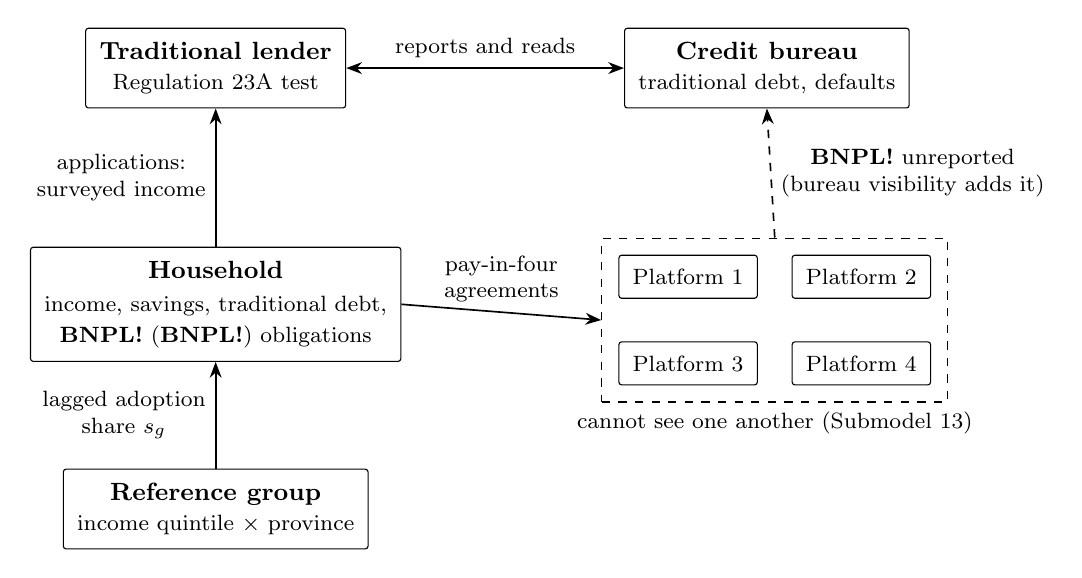
\begin{tikzpicture}[
    font=\small,
    box/.style={draw, align=center, inner sep=5pt, rounded corners=1pt},
    sees/.style={->, >=Stealth, semithick},
    gap/.style={->, >=Stealth, semithick, dashed},
    lbl/.style={font=\footnotesize, align=center},
]
\node[box, minimum width=4.0cm] (hh) at (0,0) {\textbf{Household}\\[1pt]
    \footnotesize income, savings, traditional debt,\\
    \footnotesize \ac{BNPL} obligations};
\node[box] (lender) at (0,3.0) {\textbf{Traditional lender}\\ \footnotesize Regulation 23A test};
\node[box] (bureau) at (7.0,3.0) {\textbf{Credit bureau}\\ \footnotesize traditional debt, defaults};
\node[box] (p1) at (6.0,0.35)  {\footnotesize Platform 1};
\node[box] (p2) at (8.2,0.35)  {\footnotesize Platform 2};
\node[box] (p3) at (6.0,-0.75) {\footnotesize Platform 3};
\node[box] (p4) at (8.2,-0.75) {\footnotesize Platform 4};
\node[draw, dashed, inner sep=6pt, fit=(p1)(p2)(p3)(p4),
      label={[lbl]below:{cannot see one another (Submodel 13)}}] (plats) {};
\node[box] (group) at (0,-2.6) {\textbf{Reference group}\\ \footnotesize income quintile $\times$ province};

\draw[sees] (hh) -- (lender) node[lbl, midway, left] {applications:\\ surveyed income};
\draw[sees, <->] (lender) -- (bureau) node[lbl, midway, above] {reports and reads};
\draw[sees] (hh.east) -- (plats.west) node[lbl, midway, above] {pay-in-four\\ agreements};
\draw[gap] (plats.north) -- (bureau.south) node[lbl, midway, right] {\ac{BNPL} unreported\\ (bureau visibility adds it)};
\draw[sees] (group) -- (hh) node[lbl, midway, left] {lagged adoption\\ share $s_g$};
\end{tikzpicture}
\caption{Information structure of the model}
\label{fig:visibility}
\tabnote{Boxes represent the five entity types. Solid arrows show the available information flows; dashed connections identify the benchmark's reporting gaps. The bureau excludes \ac{BNPL} unless the reporting switch in Submodel~15 is enabled. Households observe their own accounts and the lagged adoption share $s_g$ of their reference group (Submodel~11).}
\end{figure}

The traditional lender assesses an application on the household's gross income
and the scheduled service on its traditional debt, which the bureau records.
Income is the amount observed in the survey. The model does not reduce it while
a member is unemployed, so a household in a spell of unemployment is assessed on
income it is not receiving. In the benchmark the assessment excludes \ac{BNPL}
commitments \cite{nortonrose_bnpl_sa, transunion_cps_sa_2025}. The model also
omits informal borrowing, which South African households use
\cite{finscope2019}. The lender therefore applies an affordability rule to an
incomplete view of household obligations.

The boolean parameter \texttt{bnpl\_bureau\_visible}, written
$\mathbb{1}^{\text{bur}}$, controls whether active \ac{BNPL} obligations enter
this calculation. It is false in the benchmark; switching it on represents
one channel of the reporting arrangements discussed in
Section~\ref{sec:background}. A second switch, $\mathbb{1}^{\text{aff}}$,
applies the same residual-income test to each \ac{BNPL} request before it
reaches a platform. That test sees the household's traditional service and
its \ac{BNPL} instalments and arrears on every platform, whether or not the bureau switch is
on.
The model does not say how a platform would obtain that information without bureau
reporting, so the screening arm is an upper bound on what a platform's own
check could see.
Algorithms~\ref{alg:gate} and~\ref{alg:bnpl} specify how the two switches
enter lending decisions.

The bureau switch can change approval through the affordability calculation,
but it creates no credit score, changes no lending prices and cannot represent
score-based refusals. The omitted scoring channel may be material, given the
preliminary score reductions reported by \ac{FINASA} \cite{finasa_bnpl_2026}. It is
excluded from the comparison in Section~\ref{sec:scenarios} and discussed as an
extension in Section~\ref{sec:future-work}.

\subsection{Within-Tick Sequence and State Changes}
\label{sec:sequence}

Each simulation step, or tick, represents 14 days. This places the fortnightly
pay-in-four instalments directly on tick boundaries. Monthly survey flows are
converted to tick amounts using $12/26$, the ratio of months to ticks in a year. Households act in a newly randomised
order each tick, with credit applications decided as they occur. The peer-adoption
signal is updated once all households have acted, so adoption does not depend on which
group member acts first.

Each household follows seven steps (Algorithm~\ref{alg:tick}):
\begin{enumerate}
    \item Receive income, adjusted for employment shocks.
    \item Pay committed expenditure from income and savings.
    \item Accrue interest and calculate traditional and \ac{BNPL} payments due, including arrears. Minimum-payers owe the larger of interest and the minimum balance fraction; scheduled-payers owe their contractual instalment.
    \item Seek credit for a shortfall, using \ac{BNPL} first where eligible and traditional credit for the remainder. Assess distress before payment friction.
    \item Pay the \ac{BNPL} instalments that fall due, then traditional debt subject to payment friction.
    \item Spend remaining cash on discretionary consumption, up to the budget, and save the rest.
    \item Draw any want-driven \ac{BNPL} purchase and update balances, arrears, distress and default.
\end{enumerate}

The order determines how a shortfall develops. Because committed expenditure is
paid first, essential living costs can leave too little cash for debt service,
consistent with a cash-flow approach to distress \cite{madeira2018chile}.
Credit applications precede repayment, so borrowing can cover that gap.
Distress is assessed before payment friction,
so skipping an otherwise affordable instalment does not itself classify a
household as unable to pay.

Distress and arrears are distinct states. A household is distressed if it cannot
cover committed expenditure from opening cash and income, or cannot meet the
debt service due after seeking credit. A committed-expenditure shortfall is
recorded as distress and is not carried forward. Credit raised against it is
spent on debt service and then on discretionary consumption, and any remainder is
saved; a robustness arm spends it on the unpaid committed expenditure first
(Section~\ref{sec:results-effect}). Arrears track unpaid debt obligations through the \ac{CCMR}
age bands. Default occurs after seven consecutive distressed ticks, or 98 days,
and blocks all further credit. The duration is chosen to approximate the
90-day impairment convention at a 14-day resolution; the distress rule is not
identical to an account being 90 days in arrears. Default is permanent within a
run and is counted from the first tick, so the default rate at the final tick is
the share of all households that defaulted at any point in the two years.

\subsection{Credit and Adoption Mechanisms}
\label{sec:submodels}

Table~\ref{tab:submodels} sets out the seventeen operational submodels; the
initial population is constructed in Section~\ref{sec:population}.

\begingroup
\setlength{\tabcolsep}{4pt}
\small
\begin{longtable}{L{2.35cm}L{4.75cm}L{2.3cm}L{4.0cm}}
\caption{Submodel specification}
\label{tab:submodels} \\
\multicolumn{4}{p{13.4cm}}{\footnotesize The seventeen submodels, each with its rule, source and parameters. Behavioural rules are either grounded in literature or flagged as assumptions, and free parameters are sourced, derived, fitted or assumed, as defined in the note to Table~\ref{tab:param-register}, which gives each parameter's default value, provenance and sweep range. Bold marks assumptions with no literature anchor; the last column states which are swept. Submodels 4, 5, 10, 11 and 13 are elaborated in the text and Submodel 15 in Section~\ref{sec:scenarios}; the rest are given in full as pseudocode in Appendix~\ref{app:pseudo-main}.} \\
\toprule
\textbf{Submodel} & \textbf{Rule} & \textbf{Source} & \textbf{Parameters and validation} \\
\midrule
\endfirsthead
\toprule
\textbf{Submodel} & \textbf{Rule} & \textbf{Source} & \textbf{Parameters and validation} \\
\midrule
\endhead
\bottomrule
\endfoot

1. Income and shock & Surveyed income is static. Each employed member of a wage-dominant household separates with a per-tick probability, and the household loses that member's share of its wage component until re-employment. Households whose income is mainly grants or other non-wage income are exempt, because the shock is a job separation. & \cite{madeira2018chile, statssa_lmd_2022} & Income-shock probability fitted to the \ac{CCMR} 90+ band and reported against the \ac{QLFS} 2017 separation band of 0.54--1.17\% per tick. No magnitude parameter: the loss is the observed wage component. Re-employment hazard 1.87\% per tick from \ac{QLFS} 2017 Q3--Q4 flows. Single-tick non-persistent shock kept as a robustness arm. \\
\addlinespace
2. Consumption & Two tiers. Committed expenditure (food, rent) is an incompressible floor; discretionary spending compresses to zero before any instalment is missed for lack of cash. & Data layer (Section~\ref{sec:population}) & Floor of zero; not swept. \\
\addlinespace
3. Borrowing trigger & Traditional credit is sought only for realised shortfalls. \ac{BNPL} adds a want-driven path whose probability can rise with peer adoption. & \cite{ackert2025bnpl, dehaan2024bnpl} & $q_{\text{base}}$, $\beta$; see Submodel 11. \\
\addlinespace
4. Borrowing amount & Shortfall path: \textbf{structural assumption} with no anchor located; households request the exact shortfall. Want-driven path: purchase size is drawn lognormally with mean $\kappa$ times the household's own monthly discretionary budget, so purchase size inherits the population's heterogeneity. & \cite{statssa_ies_2023} & Sweeps: shortfall / $+25\%$ / $+$ one tick of committed expenditure; $\kappa = 0.139$ (derived from \ac{IES} 2022/23 \ac{COICOP} shares) swept 0.07--0.28; dispersion 0.6 (assumption); sizing base swept discretionary / income. Realised mean order checked against R992 (2017 Rands), an average order value we derive by dividing Weaver Fintech's disclosed cumulative gross merchandise value by its disclosed transaction count and deflating to 2017 \cite{weaver2025iar}. \\
\addlinespace
5. Lender choice & Eligible households take \ac{BNPL} first, up to $\kappa$ times their monthly discretionary budget, an assumed ceiling on the amount financed. An agreement frees three quarters of its value in cash, since a quarter is paid at checkout. The household asks the traditional lender for the amount it still lacks. The no-\ac{BNPL} baseline uses traditional credit only. & \cite{ackert2025bnpl} & The cap is an \textbf{assumption}; an uncapped arm is crossed with the three Submodel~4 rules. Asking the traditional lender for the whole remainder is an \textbf{assumption}. Compared with Pattern~1 (Table~\ref{tab:patterns}). \\
\addlinespace
6. Repayment and arrears & Scheduled-payers pay the full amortised instalment. Minimum-payers pay the larger of accrued interest and 5\% of balance per month, tick-scaled; the fraction is an \textbf{assumption}, since neither the \ac{NCA} nor any located source prescribes a formula. Unpaid amounts accrue as arrears in \ac{CCMR} age bands. Payment friction skips an affordable traditional instalment with fixed probability. & \cite{Keys2019, Kuchler2021} & Minimum-payer share 0.29 (swept 0.20--0.40); minimum fraction swept 0.025--0.10. Friction is the second fitted parameter, calibrated to the \ac{CCMR} 1--30 day band; it applies to traditional debt only, since \ac{BNPL} auto-debits a card. \\
\addlinespace
7. Distress and default & Distress records an unpaid committed-expenditure shortfall before borrowing, or unmet debt service due after borrowing, assessed before payment friction. Seven consecutive distressed ticks trigger default; a defaulted household is refused all further credit. & \cite{madeira2018chile} & $k=7$ ticks (98 days), the first tick boundary at or past the 90-day impairment convention; $k=4$ (56 days, the tick boundary nearest the 60-day band) swept. \\
\addlinespace
8. Heterogeneity & No behavioural parameter varies by household type. Heterogeneity enters through the data layer: income, budgets, balances and financial-inclusion flags. The minimum-payer archetype is assigned uniformly at random. & -- & No continuous present-bias parameter: no local calibration data. \\
\addlinespace
9. Credit-granting gate & The Regulation 23A residual-income test, applied at household level; all-or-nothing. New credit is priced as unsecured (repo plus 21 percentage points, 25-month term), matching Section~\ref{sec:servicing}. A granted loan is booked onto the household's consolidated balance, raising the balance and scheduled service and reweighting its rate, so each grant reduces the headroom left for the next. & \cite{sa_ncr_affordability_2015} & No free parameter; the statutory expense table is hard-coded and asserted against the regulation's published worked examples. \\
\addlinespace
10. Information asymmetry & The bureau records traditional debt and defaults only. The traditional lender cannot observe \ac{BNPL}. & \cite{nortonrose_bnpl_sa, transunion_cps_sa_2025} & \texttt{bnpl\_bureau\_visible} boolean (default off, the pre-2026 position); the bureau-visibility scenario of Submodel 15. \\
\addlinespace
11. Peer influence & $q_i(t) = \mathrm{clip}(q_{\text{base}} + \beta s_{g(i)}(t-1), 0, 1)$ within reference groups, where $s_g$ is measured on the group's \ac{BNPL}-eligible members. A heterogeneous-threshold variant, specified before the final run, is the structural alternative, run on the same access grids. & \cite{ackert2025bnpl, cardaci2018inequality, granovetter1978threshold} & $\beta=0$ control arm reported in all comparisons; the threshold arm reports its own $\gamma=0$ row. \\
\addlinespace
12. \ac{BNPL} eligibility & Banked households only; a light automated screen in place of the Regulation 23A test. Platforms also refuse a defaulted household, an \textbf{assumption}. Per-order cap R9{,}927 (2017 Rands; R15{,}000 at current prices), an \textbf{assumption}; rolling limit $\lambda = 0.10$ of monthly income per platform, set for each household, following providers' disclosed per-customer limits but without their ``grow'' step. & \cite{payflex_terms, payjustnow_terms, homechoice2024ir} & Access capped at the imputed 82.8\% banked share. At the default of 0.10, four per-platform limits sum to 40\% of monthly income, close to the 39\% we obtain by expressing Woolard's illustrative figure of about \pounds1{,}000 of \ac{BNPL} credit amassed across several lenders as a share of UK median monthly household disposable income, equivalised, in the year to March 2020 \cite{woolard2021, ons_income_fye2020}. $\lambda$ is swept 0.1--1.0 and reported against a 0.10--0.48 band whose upper end is Afterpay's maximum of A\$2{,}000 as a share of Australian median monthly household disposable income, equivalised, in 2019--20 \cite{asic2020rep672, abs_income_2019_20}. Equivalised income is below the income of a household with more than one member, so both shares overstate the limits relative to the household income that $\lambda$ multiplies. Order-cap and limit binding rates reported by quintile. \\
\addlinespace
13. Stacking & Each request goes to the platforms in a random order, redrawn for every request, and what one platform does not finance passes to the next. There is no aggregate limit, and no platform sees another's exposure. The routing rule is an \textbf{assumption}. & Follows Submodel 10 & Platforms swept 1--6 (default 4); a loyal-routing arm tries platforms already owed first; stacking depth compared with the \ac{CFPB} share in Section~\ref{sec:data-validation}. \\
\addlinespace
14. \ac{BNPL} repayment & Exogenous pay-in-four: 25\% at checkout, then 25\% at each of the next three ticks, interest-free. On a want-driven purchase the checkout debit must clear, so the order is truncated to what the household can fund. Late fees of R125.74 per tick (2017 Rands), capped per agreement at the lower of R188.61 and half the purchase price; a household that exhausts the cap is cut off by that platform only. & \cite{payflex_terms} & No free parameters; instalments fall on tick boundaries. \\
\addlinespace
15. Scenario switches & Bureau visibility ($\mathbb{1}^{\text{bur}}$: \ac{BNPL} obligations enter the traditional lender's Regulation 23A test) and mandatory affordability screening ($\mathbb{1}^{\text{aff}}$: the Regulation 23A test applied to \ac{BNPL} requests), each alone and both together (Section~\ref{sec:scenarios}). Two further levers, a cooling-off window and a cap on platforms owed, are in Appendix~\ref{app:levers}. & \cite{businessday_bnpl_2026, fca_ps26_1, woolard2021} & The two regulatory switches are binary; each arm is compared with the benchmark at $\beta = 0$ and $\beta = 1$. \\
\addlinespace
16. Macro environment & Static. The repurchase rate is fixed at 7.00\%, freezing statutory maximum interest rates. & Experimental design (Section~\ref{sec:purpose}) & Exogenous constraint. \\
\addlinespace
17. Activation order & Random, re-drawn each tick; applications decided inline as each household acts. & \cite{comer2013activation, alizadeh2015activation} & Fixed-order robustness arm (Appendix~\ref{app:supplementary}). \\
\end{longtable}
\endgroup

\subsubsection*{Submodels 4 and 5: Borrowing on a Shortfall}
\label{sec:amount}

When a household faces a shortfall, Submodel~4 determines how much it requests.
By default, the request equals the shortfall. Two alternatives add either 25\% or one
tick of committed expenditure. No study we found identifies the appropriate
rule, so all three are compared in the sensitivity analysis
(Section~\ref{sec:results-robustness}).

Submodel~5 determines which lender receives the request. An eligible household
uses \ac{BNPL} first, up to $\kappa$ times its monthly discretionary budget.
\ac{BNPL} cannot pay rent or an instalment directly. It relieves a shortfall
because the household finances a purchase it would otherwise have paid for in
cash. An agreement of value $F$ takes $F/4$ at checkout and leaves $3F/4$ in the
household's hands, so it covers $3F/4$ of the shortfall. The household asks the
traditional lender for the amount it still lacks, and the lender grants or
refuses that amount in full under Submodel~9. A refusal leaves the remainder
unpaid, and the household is recorded as distressed in that tick. The request
for the whole remainder is an assumption.

\ac{BNPL} users are disproportionately liquidity-constrained
\cite{hayashi2025constraints, dehaan2024bnpl}, which is the reason for the
shortfall path; no located study measures how much of a shortfall they finance
with it. Because \ac{BNPL} finances retail purchases and not general spending,
the model caps the amount financed for a shortfall at the mean want-driven
purchase. No empirical
maximum was located, so the sensitivity analysis repeats each borrowing-amount rule with the cap removed, and a further arm removes \ac{BNPL} from the shortfall path altogether.

\subsubsection*{Submodel 11: Peer Influence}
\label{sec:peer-influence}

Peer influence changes the probability of a want-driven purchase. Let
$s_g(t-1)$ be the share of eligible households in reference group $g$ holding
an active \ac{BNPL} balance at the previous tick. Using eligible households
as the denominator separates this signal from the group's overall banking
rate. Household $i$'s purchase propensity is:

\begin{equation}
    q_i(t) = \mathrm{clip}\!\left(q_{\text{base}} + \beta \, s_{g(i)}(t-1),\; 0,\; 1\right).
    \label{eq:peer}
\end{equation}

A positive
$q_{\text{base}}$ allows borrowing to begin before anyone in the group has
adopted. The coefficient $\beta$ determines how strongly the household responds
to others' adoption. Evidence on social approval and consumption emulation
supports the channel \cite{ackert2025bnpl, cardaci2018inequality} but does not
identify its strength, so both parameters are swept. The defaults are
$q_{\text{base}}=0.05$ and $\beta=0$, the no-peer control.

A Granovetter-style threshold rule provides a structural alternative
\cite{granovetter1978threshold}. Under this rule, the propensity rises to
$q_i = \mathrm{clip}(q_{\text{base}} + \gamma,0,1)$ when the lagged group
share reaches the household's threshold. Thresholds are drawn from
$\mathcal{N}(\mu_\theta, \sigma_\theta^2)$, with defaults $\mu_\theta=0.30$ and
$\sigma_\theta=0.20$, and clipped to $[0,1]$, so households with a negative draw
respond immediately. The sweeps vary threshold dispersion ($\sigma_\theta$),
and separate arms vary the mean. Setting $\gamma=0$ removes the threshold response; the threshold arms use $\gamma=0.3$.

\subsubsection*{Submodel 13: Stacking}
\label{sec:stacking}

A household sends each \ac{BNPL} request to the platforms in a random order,
redrawn for every request. The first platform finances as much as its order cap
and its limit for that household allow, and any remainder passes to the next.
Each platform limits only its own exposure, and the benchmark has no aggregate
limit. A household that borrows again before an earlier agreement is repaid will
therefore usually owe more than one platform: with $P$ platforms, a second
request reaches a different platform first with probability $(P-1)/P$.

No rule assigns a household a number of platforms, and the routing rule alone
determines how overlapping agreements are spread across them. The stacking
measures therefore show how often a household's agreements overlap, and carry no
information about why a household would use several providers. No evidence on
how South African households choose among providers was located, so random
routing is an assumption. A robustness arm uses the opposite rule: a household
tries the platforms it already owes first and moves to another only when a limit
binds (Section~\ref{sec:results-stacking}).

We vary the number of platforms from one to six. One platform rules out
cross-platform stacking but still permits several agreements on that platform,
which separates the number of platforms from the number of overlapping
agreements. Section~\ref{sec:data-validation} compares the stacking measures
with the \ac{CFPB} estimate and discusses the differences in definitions,
markets and observation periods.

\subsection{Implementation and Verification}
\label{sec:implementation}

The model is implemented in Python using Mesa. The lending gate reuses the affordability function
from the construction of scheduled debt service, keeping the two calculations
consistent. The parameter register in Appendix~\ref{app:specification} is
generated from the code's declarations.

Automated checks cover cash and debt accounting, arrears transitions,
Regulation 23A worked examples, pay-in-four repayments, late-fee caps, the
shortfall path and the platform-cap lever of Appendix~\ref{app:levers}. Several follow one household with
a hand-set balance sheet through a tick and compare each balance with its value
calculated by hand. Boundary checks disable \ac{BNPL}, remove peer influence
($\beta=0$ or $\gamma=0$), and restrict access to one platform. All checks pass
on the submitted code.

\section{Calibration and Empirical Grounding}
\label{sec:calibration}

This section answers RQ1. We construct the population from South African survey data, assign debt-service
and product parameters, fit two parameters to the baseline arrears profile, and
then check what the model reproduces beyond those targets.

Table~\ref{tab:param-taxonomy} classifies the inputs by provenance, and
Appendix~\ref{app:specification} gives the full register.

\begin{table}[H]
\centering
\caption{Provenance of model inputs}
\label{tab:param-taxonomy}
\tabnote{The five categories of model input, grouped by provenance, with the principal members of each and where each is documented. The order does not rank reliability. ``Imported'' means estimated on a foreign population and applied to South African households without local evidence; ``swept'' means that no source fixes the value, and sensitivity comparisons examine a range alongside the default value. The parameter register (Table~\ref{tab:param-register}) records the class of every individual parameter.}
\begin{tabular}{L{2.2cm}L{6.9cm}L{4.3cm}}
\toprule
\textbf{Class} & \textbf{Principal members} & \textbf{Documented in} \\
\midrule
Observed & Household income, expenditure, savings and debt (\ac{NIDS} 2017); financial-inclusion flags (\acs{FinScope} 2019); statutory rate ceilings and the Regulation 23A expense table; \ac{BNPL} contract terms and late fees; the re-employment hazard (\ac{QLFS} 2017) & Sections~\ref{sec:population} and~\ref{sec:servicing}; Appendix~\ref{app:variables} \\
\addlinespace
Constructed & Scheduled debt service (amortised from stocks); income quintiles and reference groups; the purchase ratio $\kappa$ (\ac{IES} 2022/23); 2017-Rand deflation of \ac{BNPL} money parameters & Section~\ref{sec:servicing}; Appendix~\ref{app:variables} \\
\addlinespace
Imported & Minimum-payer share of 0.29; the present-bias and social-approval evidence behind payment friction and want-driven borrowing (all United States) & Section~\ref{sec:lim-transfer} \\
\addlinespace
Fitted & Income-shock probability (to the \ac{CCMR} 90+ day band); payment-friction rate (to the 1--30 day band) & Section~\ref{sec:lim-calibration} \\
\addlinespace
Swept & Peer coefficients $q_{\text{base}}$, $\beta$ and the threshold parameters; the shortfall amount rule and its \ac{BNPL} cap; the minimum-payment fraction; the rolling limit $\lambda$ & Sections~\ref{sec:lim-calibration} and~\ref{sec:results-robustness} \\
\bottomrule
\end{tabular}
\end{table}

\subsection{Simulation Parameters}
\label{sec:sim-params}

Each run follows 5{,}000 households for 52 fortnightly ticks, two years.
Arrears, savings and volume measures exclude a 12-tick burn-in; default is counted
from the first tick (Section~\ref{sec:sequence}). Each configuration has
twenty replications, using seeds $s_0+i$ with a fixed starting seed for each
group of arms; the variance decomposition of Section~\ref{sec:results-robustness}
has two per design point. The four scenario arms of Section~\ref{sec:scenarios}
have one hundred, because the differences between them are smaller than twenty
replications resolve. Arms within a group share seeds and population size, and we
difference them seed by seed; because arms diverge once their random draws differ,
this pairing reduces the standard error little. The scenario arms, the cap arms, the
threshold-mean arms and each group of sensitivity arms have their own seed blocks,
given in the table notes, and we treat differences across blocks or population sizes
as independent. Thresholds use a separate random stream, so control arms reproduce
exactly across threshold dispersion. Reported dispersion is simulation variance only
and excludes uncertainty in the data and assumptions.

\subsection{The Household Population}
\label{sec:population}

Monetary values are in 2017 South African Rands (R),
the year of the primary survey.

\subsubsection*{Primary Dataset: NIDS Wave 5}
\label{sec:backbone}

The starting point is \ac{NIDS} Wave 5 \cite{nids_w5_2018}. Filtering the
13{,}719 records for reported income, valid household size and positive sampling
weights leaves 10{,}841 households. All 2{,}878 excluded records have zero or
missing weights. Applying the survey weights gives
18.67 million households and roughly 56.5 million individuals.

We construct monthly income, its dominant source, committed expenditure,
discretionary expenditure, liquid savings and traditional debt. Income sources
are grouped as wage, grant, or other. Food and rent paid form
committed expenditure; other non-food cash spending, including transport and
utilities, is treated as discretionary because \ac{NIDS} offers no finer split.
Financial assets provide the savings proxy and are winsorised at the 99th
percentile. Outstanding financial debt supplies the traditional balance.

Imputed rent is excluded because it is not a cash payment. Asset, debt and rent
fields are recorded only for holders, so missing values are set to zero;
Section~\ref{sec:data-validation} tests the aggregate consequence. Households are grouped into per-capita income
quintiles. Appendix~\ref{app:variables} records the fields, formulas and
missing-data treatment, including the servicing calculation introduced in
Section~\ref{sec:servicing}.

\subsubsection*{Imputing Financial Inclusion: FinScope 2019}
\label{sec:match}

The model also needs banking status and a consistent set of credit-product
indicators. We impute these from the 2019 \ac{FinScope} \cite{finscope2019}.
Banked status determines eligibility for \ac{BNPL}, so the imputed banked share
of 82.8\% caps holding in the constructed population. Five further flags identify store cards, revolving
credit, hire purchase, short-term loans and personal loans. These determine the
terms assigned in Section~\ref{sec:servicing}.

Figure~\ref{fig:cell-donor} shows the matching procedure. Both surveys are
partitioned by per-capita income quintile and province. Each \ac{NIDS} household
draws one donor from the corresponding cell, with probability proportional to
the donor's survey weight (seed: 42). All 45 cells contain at least 30 candidates,
so no draw requires a coarser match.

All six flags come from the same donor. This preserves combinations
observed in \ac{FinScope} and reproduces its weighted within-cell distribution
in expectation. \ac{FinScope} records one adult's holdings, so flags understate
holding in households with several adults. The match does not recover relationships with
recipient characteristics omitted from it, such as urban or rural location; within a cell, flags
are assigned without regard to them. Using 2019 banking data may also
overstate access in 2017. Appendix~\ref{app:matching} explains these assumptions
and reports donor reuse.

\begin{figure}[H]
\centering
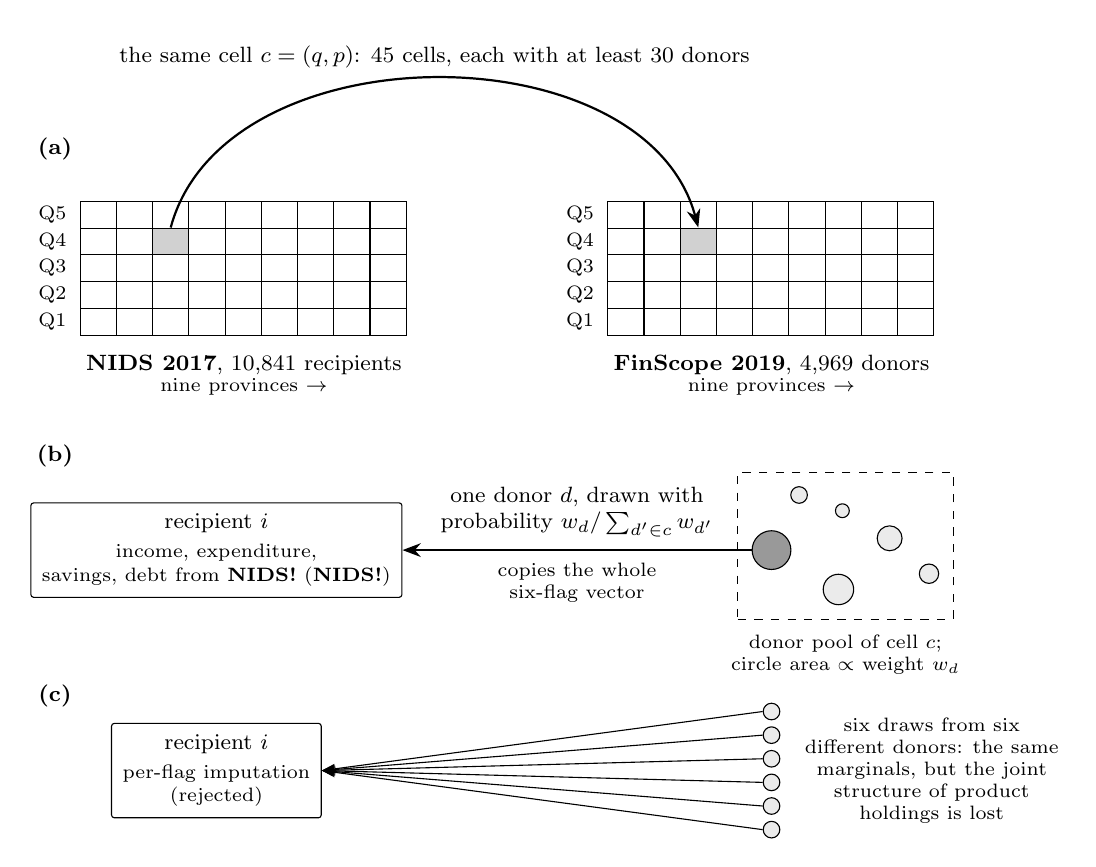
\begin{tikzpicture}[font=\footnotesize, >=Stealth,
  cell/.style={draw, minimum width=0.46cm, minimum height=0.34cm, inner sep=0pt},
  hl/.style={fill=black!18},
  rec/.style={draw, rounded corners=1pt, align=center, inner sep=4pt},
  donor/.style={circle, draw, fill=black!8, inner sep=0pt},
  lbl/.style={align=center}]
% ---- panel (a): the same partition of both surveys --------------------------
\node[lbl] at (-0.55,2.2) {\textbf{(a)}};
\foreach \x in {0,...,8} \foreach \y in {0,...,4} {
  \node[cell] at (\x*0.46, \y*0.34) {};
  \node[cell] at (6.7+\x*0.46, \y*0.34) {};
}
\node[cell, hl] (rcell) at (2*0.46, 3*0.34) {};
\node[cell, hl] (dcell) at (6.7+2*0.46, 3*0.34) {};
\foreach \y/\l in {0/Q1,1/Q2,2/Q3,3/Q4,4/Q5} {
  \node[left, font=\scriptsize] at (-0.28,\y*0.34) {\l};
  \node[left, font=\scriptsize] at (6.42,\y*0.34) {\l}; }
\node[lbl] at (1.85,-0.68) {\textbf{NIDS 2017}, 10{,}841 recipients\\[-2pt] \scriptsize nine provinces $\rightarrow$};
\node[lbl] at (8.55,-0.68) {\textbf{FinScope 2019}, 4{,}969 donors\\[-2pt] \scriptsize nine provinces $\rightarrow$};
\draw[->, thick] (rcell.north) to[out=75, in=105] node[midway, above, lbl]
  {the same cell $c = (q, p)$: 45 cells, each with at least 30 donors} (dcell.north);
% ---- panel (b): one donor, the whole vector ---------------------------------
\node[lbl] at (-0.55,-1.7) {\textbf{(b)}};
\node[rec] (recip) at (1.5,-2.9) {recipient $i$\\[1pt] \scriptsize income, expenditure,\\[-1pt] \scriptsize savings, debt from \ac{NIDS}};
\node[donor, minimum size=14pt, fill=black!40] (d3) at (8.55,-2.9) {};
\node[donor, minimum size=6pt]  (d6) at (8.9,-2.2) {};
\node[donor, minimum size=5pt]  (d1) at (9.45,-2.4) {};
\node[donor, minimum size=9pt]  (d2) at (10.05,-2.75) {};
\node[donor, minimum size=7pt]  (d4) at (10.55,-3.2) {};
\node[donor, minimum size=11pt] (d5) at (9.4,-3.4) {};
\node[draw, dashed, fit=(d1)(d2)(d3)(d4)(d5)(d6), inner sep=5pt,
  label={[lbl, font=\scriptsize, yshift=-2pt]below:donor pool of cell $c$;\\ circle area $\propto$ weight $w_d$}] (pool) {};
\draw[->, thick] (d3.west) -- (recip.east)
  node[midway, above, lbl, yshift=1pt] {one donor $d$, drawn with\\ probability $w_d / \sum_{d' \in c} w_{d'}$}
  node[midway, below, lbl, font=\scriptsize, yshift=-1pt] {copies the whole\\ six-flag vector};
% ---- panel (c): the rejected alternative ------------------------------------
\node[lbl] at (-0.55,-4.75) {\textbf{(c)}};
\node[rec] (recip2) at (1.5,-5.7) {recipient $i$\\[1pt] \scriptsize per-flag imputation\\[-1pt] \scriptsize (rejected)};
\foreach \k/\ypos in {1/-4.95,2/-5.25,3/-5.55,4/-5.85,5/-6.15,6/-6.45} {
  \node[donor, minimum size=6pt] (e\k) at (8.55,\ypos) {};
  \draw[->, thin] (e\k.west) -- (recip2.east); }
\node[lbl, right, font=\scriptsize] at (8.85,-5.7) {six draws from six\\ different donors: the same\\ marginals, but the joint\\ structure of product\\ holdings is lost};
\end{tikzpicture}
\caption{The cell-donor match}
\label{fig:cell-donor}
\tabnote{Panel (a): both surveys share 45 cells by per-capita income quintile and province, each with at least 30 donors. Panel (b): one donor per recipient, drawn in proportion to survey weight (circle area), supplies the whole six-flag vector. Panel (c): the rejected per-flag alternative keeps the marginals but loses the joint structure of product holdings, which prices opening traditional debt. Appendix~\ref{app:matching} gives the procedure formally.}
\end{figure}

National imputed rates differ from their targets by at most 1.8 percentage
points (Table~\ref{tab:imputation_errors}). The largest gap across the thirty
quintile-by-indicator cells is 2.3 points (Figure~\ref{fig:inclusion-fidelity}).

\begin{table}[H]
\centering
\caption{National rates for the six imputed indicators}
\label{tab:imputation_errors}
\tabnote{This table compares the national rate of each imputed indicator in three populations: the \ac{FinScope} 2019 target, weighted by its survey weight; the 10{,}841-household synthetic population after matching, weighted by \ac{NIDS} survey weight; and the unweighted 5{,}000-agent resample used in the simulation. The difference column is synthetic less \ac{FinScope}, in percentage points, computed before rounding; the tolerance is 3 percentage points (Table~\ref{tab:validation}). Because the match draws donors within the same quintile-by-province cell in proportion to weight, agreement here is expected by construction: it tests the implementation, not the population's external validity (Appendix~\ref{app:matching}).}
\begin{tabular}{lrrrr}
\toprule
\textbf{Imputed indicator} & \textbf{FinScope 2019} & \textbf{Synthetic} & \textbf{Agents} & \textbf{Difference} \\
 & \textbf{(\%)} & \textbf{(\%)} & \textbf{(\%)} & \textbf{(pp)} \\
\midrule
Banked status    & 82.4 & 82.8 & 82.8 & 0.4 \\
Store card       & 20.8 & 22.6 & 21.8 & 1.8 \\
Revolving credit &  3.7 &  4.1 &  3.8 & 0.5 \\
Hire purchase    &  6.5 &  6.9 &  6.5 & 0.5 \\
Short-term loan  &  2.7 &  3.4 &  3.3 & 0.6 \\
Personal loan    &  2.1 &  2.3 &  2.3 & 0.2 \\
\bottomrule
\end{tabular}
\end{table}

\begin{figure}[htbp]
\centering
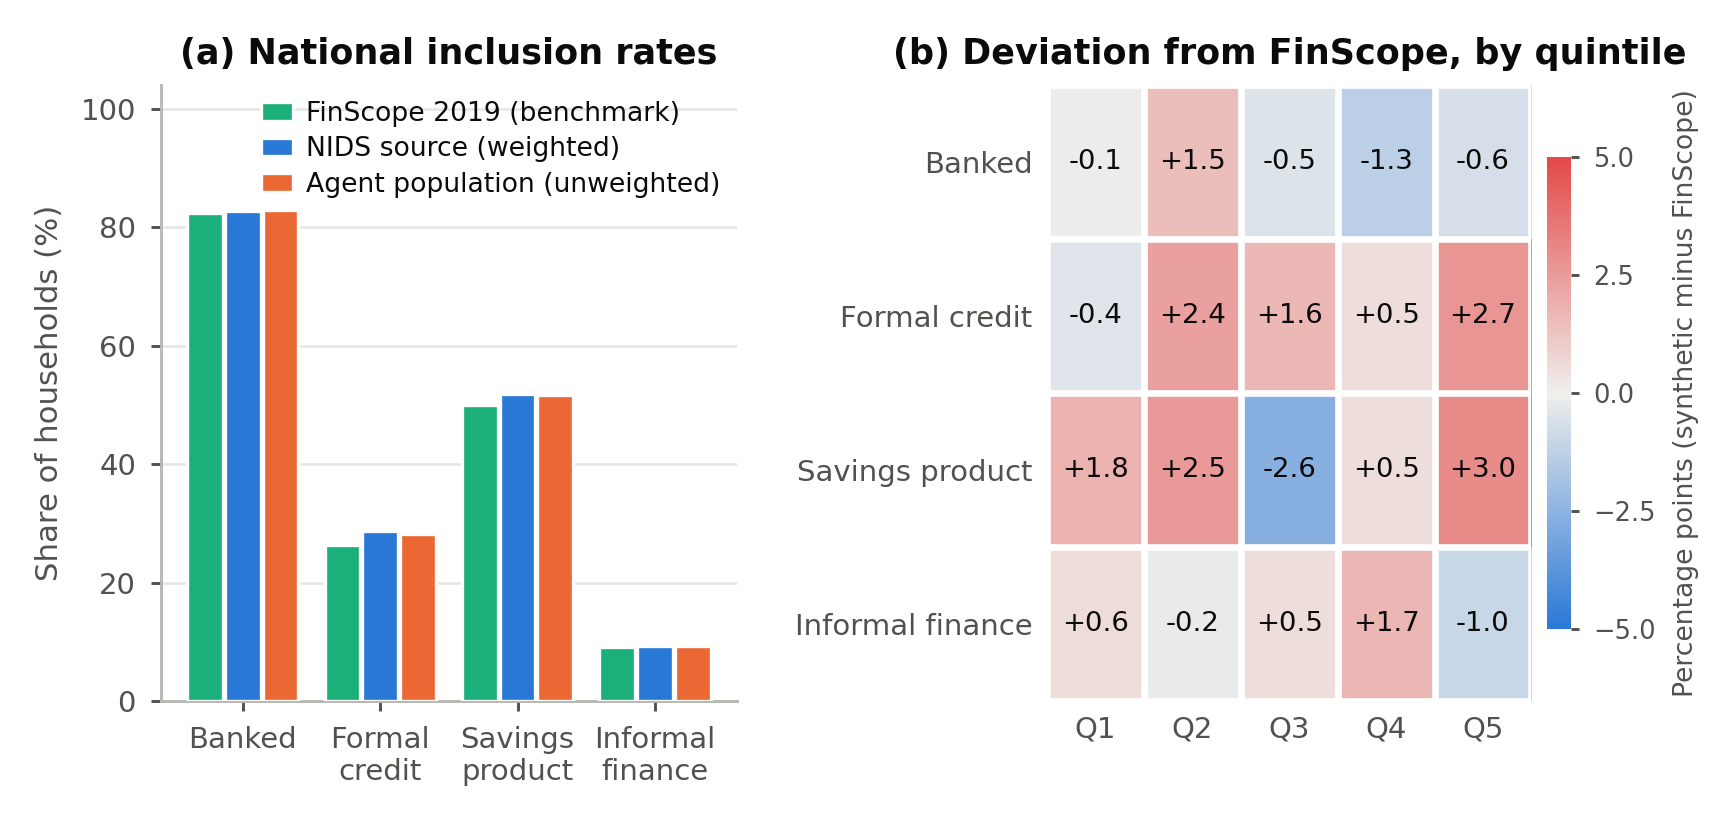
\includegraphics[width=\textwidth]{figures/fig_inclusion_fidelity.png}
\caption{Fidelity of the imputed indicators}
\label{fig:inclusion-fidelity}
\tabnote{Panel (a) compares the national rate of each of the six imputed indicators across the \ac{FinScope} 2019 target, the weighted synthetic population and the unweighted 5{,}000-agent population, as in Table~\ref{tab:imputation_errors}. Panel (b) shows the synthetic-less-\ac{FinScope} gap for each indicator within each per-capita income quintile, thirty cells in all; the largest single deviation is 2.3 percentage points against a tolerance of 5. Quintiles are the weighted \ac{NIDS} bounds of Appendix~\ref{app:variables}.}
\end{figure}

\subsubsection*{Population Resampling}
\label{sec:resample}

We sample $N=5{,}000$ agents with replacement from the 10{,}841 households,
using probabilities proportional to survey weights (seed: 20260818). Simulation
statistics can then be calculated without applying weights again.
Figure~\ref{fig:pop-fidelity} compares the resample with its source; the per-capita income Gini
rises by 0.015, from 0.6514 to 0.6668.

\begin{figure}[htbp]
\centering
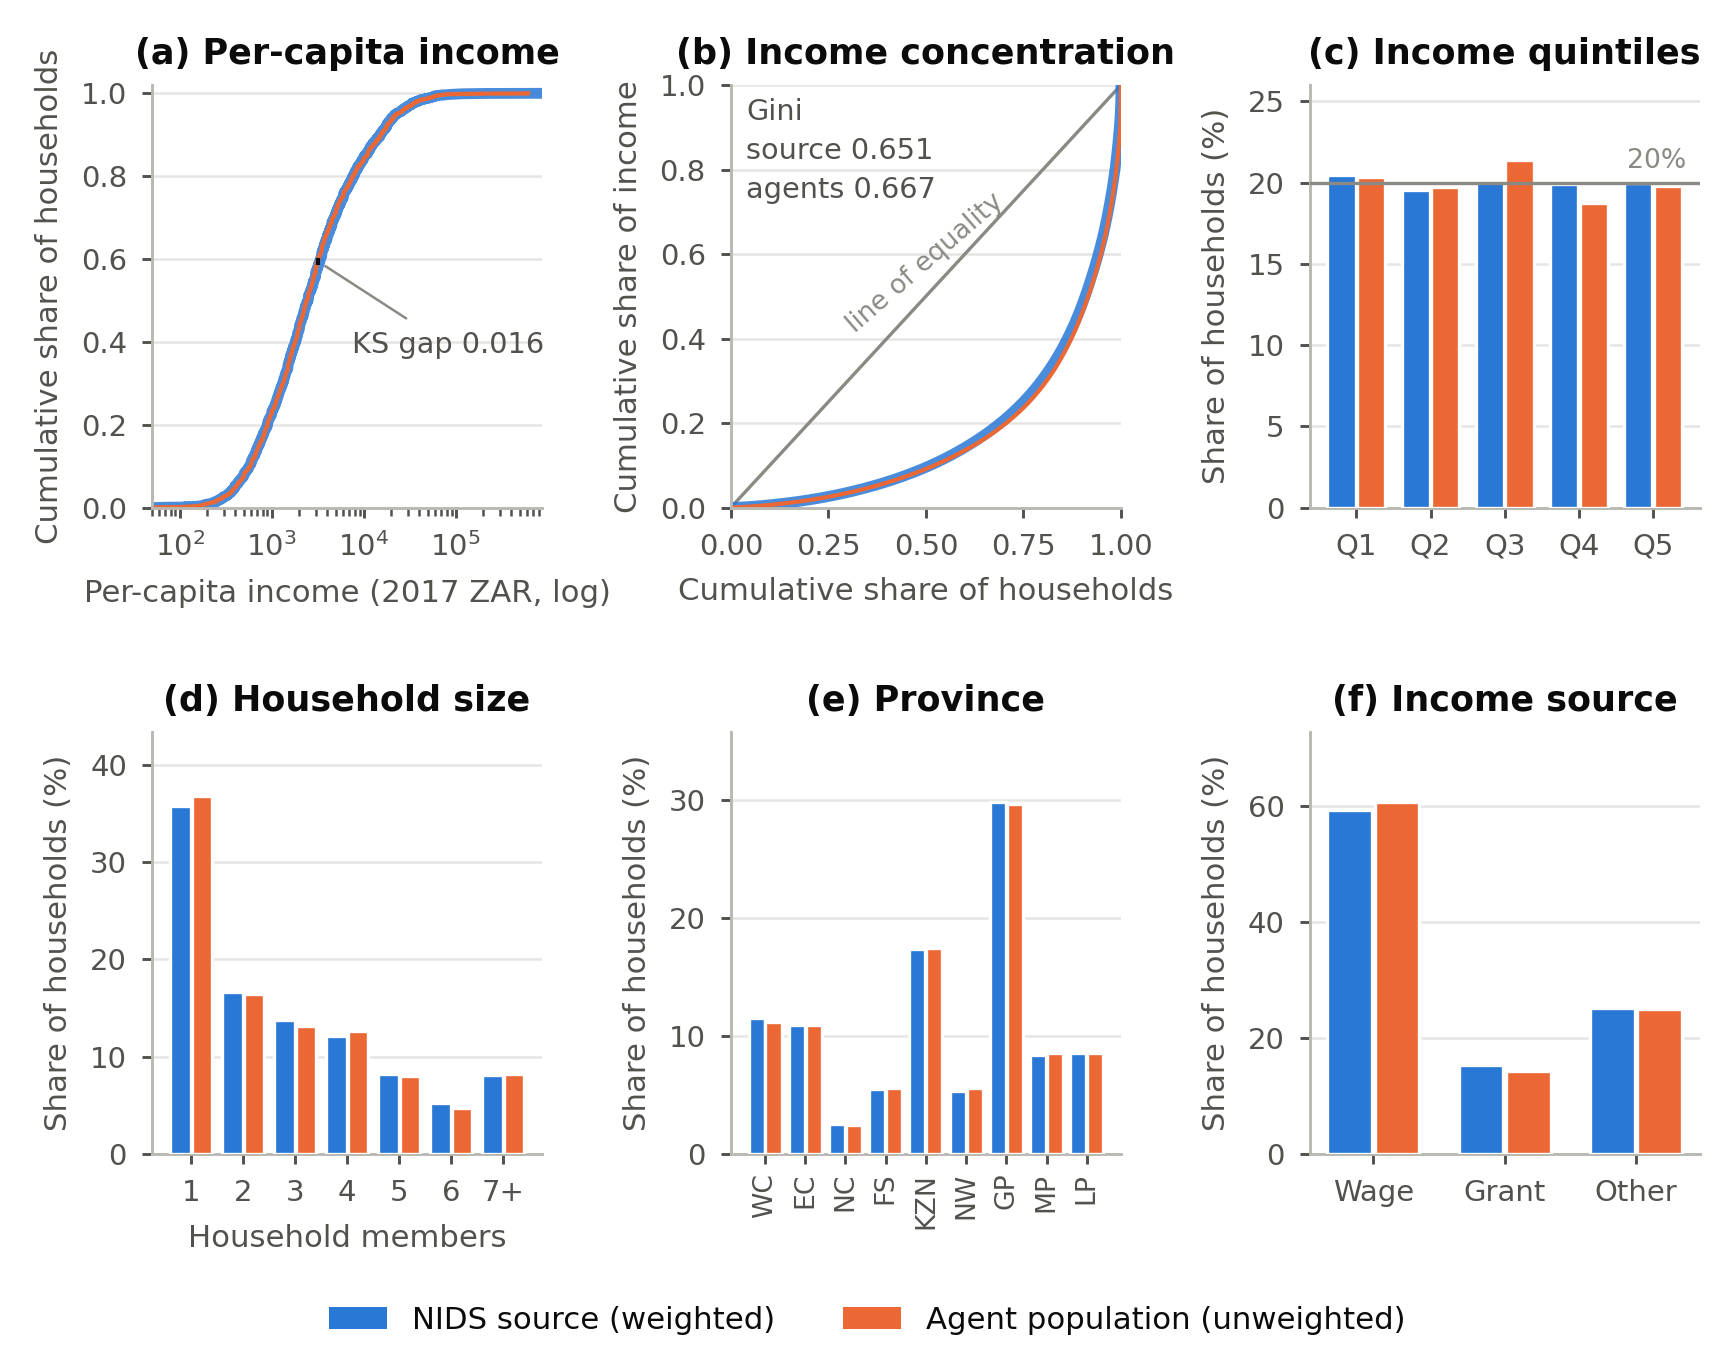
\includegraphics[width=\textwidth]{figures/fig_population_fidelity.png}
\caption{Distributional fidelity of the agent population}
\label{fig:pop-fidelity}
\tabnote{Each panel compares the unweighted 5{,}000-agent resample, drawn with replacement in proportion to \ac{NIDS} survey weight (seed 20260818) from 3{,}221 unique source records, against the weighted 10{,}841-household source it is drawn from. Panels (a) and (b) cover the per-capita income distribution and its concentration; panels (c) to (f) cover income quintile, household size, province and primary income source, the categorical attributes that gate behaviour and define the reference groups in the simulation. The Kolmogorov--Smirnov distance in (a) is 0.016, the largest categorical deviation across the 24 sub-categories is 1.4 percentage points, and the Gini rises by 0.015, from 0.6514 to 0.6668.}
\end{figure}

\subsection{Debt-Service and Product Parameters}
\label{sec:servicing}

\ac{NIDS} provides the outstanding debt balance, but the simulation needs the
payment due each month. We reconstruct servicing using a product rate, a
repayment horizon and an affordability cap (Appendix~\ref{app:variables}).
Balances are amortised at the applicable 2017 statutory maximum \ac{APR}
\cite{sa_ncr_ratecaps_2016} over the horizons in Table~\ref{tab:credit-terms}.
The resulting payment is capped at the Regulation 23A residual-income ceiling
\cite{sa_ncr_affordability_2015}.

The statutory rates are proxies. Realised product rates were not available in
the \ac{CCMR} \cite{ncr_ccmr_2017} or the other 2017 sources consulted.
Because realised rates cannot exceed the ceilings, this choice biases
calculated payments upward. Product allocation, horizons and the cap are also
approximations, but constructed service exceeds the survey range
(Section~\ref{sec:data-validation}), so the net error is probably upward.

\begin{table}[tbp]
\centering
\caption{Interest rates and repayment horizons by product class}
\label{tab:credit-terms}
\tabnote{This table gives the annual rate and repayment horizon used to amortise each household's opening traditional debt, by the product class its \ac{FinScope} donor flags; a household holding several classes takes the unweighted mean of each. Rates are the \ac{NCA} statutory maxima at the 2017 repurchase rate of 7.00\% \cite{sa_ncr_ratecaps_2016}, not realised market rates, which were not available in the sources consulted. Horizons are either measured in \ac{NIDS} as the median ratio of the household's total financial debt to the observed monthly payment for that product ($n$ as shown), upper bounds because the numerator is the whole balance, or derived from the \ac{CCMR} stock-flow implied life, three times the gross debtors book over quarterly credit granted. Construction detail is in Appendix~\ref{app:variables}.}
\begin{tabular}{L{2.7cm}L{1.2cm}L{1.9cm}L{5.7cm}}
\toprule
\textbf{Product class} & \textbf{\ac{APR}} & \textbf{Horizon (months)} & \textbf{Provenance} \\
\midrule
Store card & 21\% & 11 & Measured in \ac{NIDS}: median total debt over observed monthly clothing-account payment, $n=782$ \cite{nids_w5_2018} \\
\addlinespace
Hire purchase & 24\% & 8 & Measured in \ac{NIDS}: median total debt over observed monthly hire-purchase payment, $n=121$ \cite{nids_w5_2018} \\
\addlinespace
Short-term loan & 60\% & 1 & \ac{FinScope} defines the product as repayable within 31 days; the \ac{CCMR} places 65.8\% of such agreements at one month or less \cite{finscope2019, ncr_ccmr_2017} \\
\addlinespace
Personal loan & 28\% & 25 & \ac{CCMR} stock-flow implied life of the unsecured book, 24.8 months \cite{ncr_ccmr_2017} \\
\addlinespace
Revolving credit & 21\% & 20 & No contractual term exists. Derived as the reciprocal of the default minimum-payment fraction, 0.05, which is swept over 0.025 to 0.10 \\
\addlinespace
Unflagged balance & 28\% & 25 & Fallback for the 74.0\% of donors flagging no specific product; mapped as personal loan \\
\bottomrule
\end{tabular}
\end{table}

The cap binds for only 3.8\% of debtors but removes 22.8\% of calculated
service (Appendix~\ref{app:var-servicing}). The non-food aggregate already
includes clothing-account, hire-purchase and vehicle payments, a median 12.6\% of
non-food outlay among the households reporting them, so adding reconstructed service
partly counts that flow twice. This overstates compressible outlay and understates
service as a share of it; the net effect on default is unsigned.

The \ac{BNPL} contract and late fees come from published provider
terms \cite{payflex_terms, payjustnow_terms}, deflated to 2017 Rands. The order cap
of R15{,}000 (R9{,}927 in 2017 Rands) is an assumption: Payflex's terms state no maximum order value, and its support
material says that the amount a customer may spend depends on an individual
assessment \cite{payflex_terms, payflex_limits}. The cap binds on 0.3\% of
platform requests at $\beta=0$. The purchase-size ratio $\kappa=0.139$ comes from the share of
discretionary spending on eligible categories in \ac{IES} 2022/23
\cite{statssa_ies_2023}. Using a share avoids converting currency amounts,
but still assumes that the spending composition transfers to 2017.
No usable South African provider estimate was located for the rolling limit.
We therefore treat $\lambda$ as an assumption, informed by Woolard's illustrative
stacked exposure \cite{woolard2021}, and sweep it from 0.10 to 1.0 (Submodel~12).

\label{sec:lim-transfer}
The behavioural evidence discussed in Section~\ref{sec:lit-behavioural}
comes from United States borrowers. It supplies the minimum-payer share of
0.29 and the case for payment friction and want-driven borrowing; we located no South
African or other developing-market estimates for these rules. We vary the minimum-payer share from 0.20 to 0.40, which shows how much
the value matters but cannot show that it transfers.
A continuous present-bias parameter is omitted because no South African
distribution was available to calibrate it.

\subsection{Estimation and Experimental Protocol}
\label{sec:lim-calibration}

We fit two parameters to two parts of the 2017-Q1 \ac{CCMR} arrears
distribution (Table~\ref{tab:ccmr}; Pattern~2 in Table~\ref{tab:patterns}).
With \ac{BNPL} disabled, the income-shock probability is fitted to the 90+ day share
and payment friction to the 1--30 day share. They primarily affect different
parts of the distribution: persistent shocks generate long arrears, while
friction produces brief payment delays. The selected values are 1.6\% and
9\% per tick. The shock probability is chosen from a grid with steps of
0.8 percentage points. A check in steps of 0.1 points places the target between
1.5\%, which gives a 90+ share of 13.93\%, and the selected 1.6\%, which gives
14.48\% (Table~\ref{tab:arrears-fit}). Both values remain fixed when \ac{BNPL} is
introduced. The fitted shock probability is about 1.4 times the upper end of the
observed separation-rate range, 0.54--1.17\% per tick, so we interpret it as a
reduced-form hazard of income loss and other distress, such as illness, unexpected
bills or family changes.

\begin{table}[H]
\centering
\caption{2017-Q1 \ac{CCMR} arrears profile}
\label{tab:ccmr}
\tabnote{The calibration target: the distribution of accounts by days in arrears for unsecured credit and credit facilities combined, first quarter of 2017, from Tables 21 and 23 of the \ac{CCMR} \cite{ncr_ccmr_2017}. The unit is the account, not the household, so the model's household-level arrears distribution over the credit-active subpopulation is compared with it for shape and scale rather than point for point. Each aggregate row sums the bands beyond its threshold.}
\begin{tabular}{lr}
\toprule
\textbf{Age band} & \textbf{Share of accounts (\%)} \\
\midrule
Current                  & 71.63 \\
1--30 days               &  8.24 \\
31--60 days              &  3.59 \\
61--90 days              &  2.32 \\
91--120 days             &  1.76 \\
120+ days                & 12.45 \\
\midrule
\emph{Aggregate: 60+ days}  & \emph{16.54} \\
\emph{Aggregate: 90+ days}  & \emph{14.21} \\
\bottomrule
\end{tabular}
\end{table}

Other inputs retain their assigned values except where varied.
Neither $q_{\text{base}}$ nor $\beta$ has a direct empirical estimate, so the
adoption rate is not identified. Only indirect comparisons are available: the
banking ceiling, the \ac{CFPB} stacking shares, and TransUnion's finding that
57\% of surveyed consumers hold a \ac{BNPL} product \cite{transunion_cir_sa_2026},
against 70.0\% of households that ever hold a balance at $\beta=0$.

\subsection{Validation}
\label{sec:data-validation}

Construction checks test whether the population preserves the properties of
its sources, and calibration checks test the fit to the two targets. External
comparisons, against quantities neither fitted nor imposed, test more than the
construction, but only as far as they measure comparable populations and outcomes. Table~\ref{tab:patterns} lists the four patterns used.

\label{sec:lim-validation}
Only Pattern~2 is both South African and matched to the model's base year.
Even here, the administrative unit is an account and the model unit is a
household. Arrears shares are calculated over credit-active households
(those holding traditional debt or arrears, 45\% at the start), while population default is tracked
separately. This improves the comparison but does not remove the unit mismatch,
which also limits interpretation of the fitted income-shock probability.

Pattern~1 is not independent of model development. Want-driven borrowing
was introduced partly because shortfall-only borrowing did not reproduce
the complementarity, so Pattern~1 serves as a diagnostic of the resulting
behaviour. Pattern~3 compares against a United Kingdom model. Pattern~4
compares zero savings with expected missed payments in a 2025 survey, which
are different outcomes. Patterns 1, 3 and 4 are therefore plausibility
comparisons.

\begin{table}[H]
\centering
\caption{Empirical patterns used to assess the model}
\label{tab:patterns}
\tabnote{The four empirical patterns, following the pattern-oriented modelling convention of the \ac{ODD} protocol. Pattern~2 is the calibration target: two parameters, the income-shock probability and the payment-friction rate, are fitted to its 90+ and 1--30 day bands, so agreement on those bands is not evidence. The third column states what the model must produce for the pattern to count as reproduced and what would falsify it.}
\begin{tabular}{L{2.4cm}L{4.2cm}L{4.8cm}L{1.5cm}}
\toprule
\textbf{Pattern} & \textbf{Empirical Observation} & \textbf{Model Analogue \& Falsification Condition} & \textbf{Source} \\
\midrule
1. Complementarity, not substitution & \ac{BNPL} adoption correlates with subsequent increases in credit-card interest and late fees. & Enabling \ac{BNPL} should elevate arrears and servicing stress on \emph{traditional} debt. A reduction falsifies the lender-choice hierarchy. Measured via servicing stress, not debt stock. & \cite{dehaan2024bnpl} \\
\addlinespace
2. Baseline arrears & 2017-Q1 arrears profile for unsecured credit and credit facilities combined. & With \ac{BNPL} disabled, the credit-active population's arrears distribution must approximate Table~\ref{tab:ccmr}. \textbf{(Calibration target)} & \cite{ncr_ccmr_2017} \\
\addlinespace
3. Non-monotonic debt burden & Debt-to-income peaks among middle-income households in independent modelling. & The aggregate debt-to-income ratio (total debt over total income per quintile, the statistic specified before the run) must peak mid-distribution rather than rising monotonically with income. & \cite{hamill2023creditcard} \\
\addlinespace
4. Savings exhaustion & 36\% of South African consumers anticipated missing a bill payment. & The share of agents reaching zero liquid savings should be of the same order. A stated expectation compared against a realised stock, so order-of-magnitude only. & \cite{transunion_cps_sa_2025} \\
\bottomrule
\end{tabular}
\end{table}

The model misses the intermediate arrears bands
(Table~\ref{tab:arrears-fit}). Both are about 1\%, compared with 3.6\% and
2.3\% in the \ac{CCMR}. The cumulative 60+ share is closer, at 15.5\%
against 16.5\%, but includes the fitted 90+ band. The profile concentrates
too heavily in brief and persistent arrears. Because households start current
and no account is written off, the 90+ band accumulates every uncured account: at
the fitted values it averages 14.48\% after burn-in but reaches 19.9\% at the final
tick. The fit therefore matches the time average of a rising stock, and matching
the two targets does not establish that arrears transitions are well represented.

% GENERATED by notebooks/scripts/build_results_tables.py from results/raw --
% do not edit by hand; re-run the script instead.
\begin{table}[H]
\centering
\caption{Baseline arrears profile against the \ac{CCMR}}
\label{tab:arrears-fit}
\tabnote{Baseline calibration results, with \ac{BNPL} disabled. Shares are over credit-active households and are compared with the account-level \ac{CCMR} target, in per cent. Means cover twenty replicates (seeds 1{,}000--1{,}019) at income-shock probability 0.016 and payment friction 0.09; the 90+ share has a replicate standard deviation of 0.40 percentage points. The shock probability is fitted on a grid with steps of 0.008: the neighbouring values 0.008 and 0.024 give 90+ shares of 11.31\% and 17.10\%. A check on the same seeds in steps of 0.001 gives 13.93\% at 0.015, so the target lies between that value and the selected one. ``Fitted'' identifies the two target bands. Unfitted bands belong to the same distribution and are not independent observations. The cumulative 60+ row includes the fitted 90+ band.}
\begingroup\setlength{\tabcolsep}{4pt}\normalsize
\begin{tabular}{lrrl}
\toprule
\textbf{Age band} & \textbf{\ac{CCMR}} & \textbf{Model} & \textbf{Status} \\
\midrule
Current & 71.63 & 75.38 & unfitted \\
1--30 days & 8.24 & 8.19 & fitted \\
31--60 days & 3.59 & 0.97 & unfitted \\
61--90 days & 2.32 & 0.99 & unfitted \\
90+ days & 14.21 & 14.48 & fitted \\
\midrule
\emph{60+ days} & \emph{16.54} & \emph{15.46} & \emph{partly fitted} \\
\bottomrule
\end{tabular}
\endgroup
\end{table}


Three external comparisons fall within the chosen tolerances: household size,
income inequality and aggregate debt (Table~\ref{tab:validation}).
Constructed servicing falls outside its tolerance, at 12.8\% of monthly outlay
against the \ac{FinScope} range of 6.1--9.8\%. That measure was not used to
fit servicing, although the survey supplies other construction inputs.
The remaining fourteen checks comprise thirteen construction checks and one
diagnostic on how often the Regulation 23A cap binds. Passing them demonstrates
the internal consistency of the construction only.

\begin{table}[H]
\centering
\caption{Data-layer validation scorecard}
\label{tab:validation}
\tabnote{Eighteen checks on the constructed population, grouped by what they test. Groups A, B and E contain thirteen construction checks on consistency, imputed marginals and resampling. The household-size row in Group A is an external comparison with the Community Survey. Group C compares with quantities that no construction step targeted. Group D bounds the debt-service construction: the first row is the share of debtors for whom the Regulation 23A cap binds, the second the servicing share of monthly outlay among indebted households, against \ac{FinScope}'s self-reported range among holders of a modelled product. Tolerances with a source: the household-size band is the 2016 Community Survey \cite{statssa_cs_2016}, the Gini interval is bounded below by the World Bank consumption-based estimate of 63.0 for 2014 as published until February 2026 (the April 2026 release revises it to 59.6 and adds 54.1 for 2022) \cite{worldbank_gini_zaf}, and the Group D range is \ac{FinScope}'s \cite{finscope2019}; the remainder are ours. Values are survey-weighted except in Group E, which compares the unweighted agents with the weighted source.}
\begin{tabular}{L{4.9cm}L{3.6cm}rrc}
\toprule
\textbf{Check} & \textbf{Metric} & \textbf{Value} & \textbf{Tolerance} & \\
\midrule
A. Quintile shares $\approx 20\%$ & max $|$share $-0.20|$ & 0.4pp & $\pm$2pp & \checkmark \\
A. Mean household size & weighted mean & 3.03 & 3.3 $\pm$0.5 \cite{statssa_cs_2016} & \checkmark \\
A. No impossible values & negative values & 0 & exact & \checkmark \\
\addlinespace
B. Banked (national) & vs FinScope & 0.4pp & $\pm$3pp & \checkmark \\
B. Store card & vs FinScope & 1.8pp & $\pm$3pp & \checkmark \\
B. Revolving credit & vs FinScope & 0.5pp & $\pm$3pp & \checkmark \\
B. Hire purchase & vs FinScope & 0.5pp & $\pm$3pp & \checkmark \\
B. Short-term loan & vs FinScope & 0.6pp & $\pm$3pp & \checkmark \\
B. Personal loan & vs FinScope & 0.2pp & $\pm$3pp & \checkmark \\
B. By-quintile flags & max over q$\times$flag & 2.3pp & $\pm$5pp & \checkmark \\
\addlinespace
C. Per-capita income Gini & weighted Gini & 0.651 & in (0.63, 0.70) & \checkmark \\
C. Aggregate debt vs \ac{CCMR} & stock $/$ in-scope book & 0.49 & in (0.30, 0.80) & \checkmark \\
\addlinespace
D. Regulation 23A cap & debtors on whom it binds & 3.8\% & $\leq$10\% & \checkmark \\
D. Debt service vs \ac{FinScope} & monthly outlay, debtors & 12.8\% & in (6.1, 9.8)\% & $\times$ \\
\addlinespace
E. Resample quintile shares & max $|$unwtd $-$ wtd$|$ & 1.3pp & $\pm$2pp & \checkmark \\
E. Resample flag rates & max $|$unwtd $-$ wtd$|$ & 0.8pp & $\pm$3pp & \checkmark \\
E. Resample income ECDF & KS max gap & 0.016 & $\leq$0.05 & \checkmark \\
E. Resample Gini & $|$agents $-$ source$|$ & 0.015 & $\leq$0.02 & \checkmark \\
\bottomrule
\end{tabular}
\end{table}

These external tolerances are broad. The income Gini of 0.651 lies in the
0.630--0.700 interval, whose lower bound is the World Bank's consumption-based Gini
for 2014 \cite{worldbank_gini_zaf} and whose upper bound is Statistics South
Africa's per-capita income Gini for 2009 \cite{statssa2019inequality}. The closest
income measures, 0.67 for 2015 and 0.66 from the 2014 wave of \ac{NIDS}
\cite{statssa2019inequality, hundenborn2018drivers}, lie 0.01 to 0.02 above the model. Synthetic debt of
R191.4 billion is 49\% of the corresponding R392.0 billion
\ac{CCMR} book \cite{ncr_ccmr_2017}. Underreporting may contribute to
this gap. Imputing missing balances at holder means would instead produce 111\%
of the administrative book, so the comparison depends on the missing-data
treatment.

Mean household size passes its tolerance but, at 3.03, is below the
Community Survey estimate of 3.3 \cite{statssa_cs_2016}, and the weighted
population contains roughly 10\% more households: 18.67 million against
16.9 million.

Some households begin in a vulnerable position. Among the 5{,}000 agents,
income does not cover committed expenditure for 3.6\%, or committed expenditure
plus scheduled service for 5.1\%, and 45.2\% have zero liquid savings. These groups
overlap, and none is a count of initial distress, which the tick sequence determines
(Section~\ref{sec:sequence}).

Table~\ref{tab:bnpl-on-checks} reports the unfitted comparisons after
\ac{BNPL} is enabled. At the final tick, 52.0\% of holders have balances on two
or more platforms. The over-the-horizon measure, 36.8\% of
households that ever held a balance, is closer in definition to the \ac{CFPB}'s measure: the share of
United States \ac{BNPL} borrowers with simultaneous loans at two or more firms
during a year, 32\% in 2021 and 33\% in 2022. The markets and observation
periods differ.

% GENERATED by notebooks/scripts/build_results_tables.py from results/raw --
% do not edit by hand; re-run the script instead.
\begin{table}[H]
\centering
\caption{Unfitted checks on the \ac{BNPL}-on model}
\label{tab:bnpl-on-checks}
\tabnote{Every comparison here is against a quantity no parameter was fitted to. Model values are means over 20 replicates, replicate standard deviation in brackets from the $\beta = 0$ arm of Table~\ref{tab:baseline-arms} unless the $\beta = 1$ arm is named; Patterns 3 and 4 use the no-\ac{BNPL} baseline. The \ac{CFPB} share is of borrowers who held simultaneous loans at more than one firm, 32\% in 2021 and 33\% in 2022 \cite{cfpb2025bnpl}. Volumes are the post-burn-in cumulative volume divided by the number of eligible (banked) households or of households that ever held a balance, annualised over the 1.53-year post-burn-in horizon; the band is the 2017-Rand provider disclosure whose customer denominator is not stated \cite{weaver2025iar}. The mean purchase is over every want-driven purchase in the run, burn-in included. The mean-purchase comparison population (all want-driven purchases), statistic, target and tolerance were specified before the run; the Q3--Q5 and Q4--Q5 means explain the gap and are not alternative comparison populations. Pattern 1 compares arms that share seeds, so its differences are paired by seed and carry one standard error; a reading of rise or fall requires a difference beyond two standard errors.}
\begingroup\setlength{\tabcolsep}{3pt}\footnotesize
\begin{tabular}{L{3.6cm}L{2.9cm}L{3.2cm}L{4.1cm}}
\toprule
\textbf{Check} & \textbf{Model} & \textbf{Comparison} & \textbf{Reading} \\
\midrule
\multicolumn{4}{l}{\emph{Stacking (Submodel 13)}} \\
Holders with balances on two or more platforms, final tick & 52.0\% & 32\% of borrowers held simultaneous loans at more than one firm (2021) & order of magnitude; ever-stacked share of households that ever held a balance 36.8\% \\
\multicolumn{4}{l}{\emph{Volume (Submodel 4)}} \\
Annual \ac{BNPL} volume per eligible household & R1{,}010 & R1{,}333--R4{,}261 (per signed-up and per active customer) & below the band; eligible households compare with the lower bound \\
Annual \ac{BNPL} volume per household that ever held a balance & R1{,}196 & as above & below the band; these households compare with the upper bound \\
Mean want-driven purchase, $\beta = 0$ & R633.16 & R992 $\pm$ 35\% (R645--R1{,}339) & 36.18\% low: outside the band; 4 of 20 replicates inside; Q3--Q5 mean R890, Q4--Q5 R1{,}186 \\
Mean want-driven purchase, $\beta = 1$ & R610.19 & as above & 38.50\% low: outside the band; 0 of 20 inside \\
\multicolumn{4}{l}{\emph{Patterns (Table~\ref{tab:patterns})}} \\
Pattern 1: traditional arrears rate, on less off & $+0.23 \pm 0.07$pp; $+0.57 \pm 0.07$pp & rise & rises \\
Pattern 1: traditional interest charged, on over off & $-1.5 \pm 0.4\%$; $-0.3 \pm 0.5\%$ & rise & falls at $\beta = 0$, no detectable change at $\beta = 1$: the pattern is not reproduced on this measure \\
Pattern 3: aggregate debt-to-income peak, no \ac{BNPL} & Q1 (0.77); Q4 second (0.69) & middle-income peak & the highest ratio is in Q1: not reproduced; the mean of ratios peaks in Q1 \\
Pattern 4: zero liquid savings & 25.7\% (no \ac{BNPL}); 25.9\% ($\beta = 0$) & 36\% expected to miss a payment & same order \\
\bottomrule
\end{tabular}
\endgroup
\end{table}


The model fails the purchase-size and volume checks. The mean want-driven
purchase is R633 against a target of R992, 36.2\% below it under a tolerance of
35\%, and four of twenty replications fall inside the band. At $\beta=1$ the
mean is R610 and no replication falls inside. Annual volume is R1{,}010 per
eligible household against a lower bound of R1{,}333, and R1{,}196 per ever-holder
against the R4{,}261 bound for active customers. The model's \ac{BNPL} market
therefore has smaller purchases and less volume per user than the provider
disclosure.

Pattern~1 holds on the arrears measure and fails on the interest measure.
Enabling \ac{BNPL} raises the traditional arrears rate by $0.23 \pm 0.07$ points at
$\beta=0$ and $0.57 \pm 0.07$ at $\beta=1$. The interest charged on traditional debt
falls by $1.5 \pm 0.4$\% at $\beta=0$, which the condition in
Table~\ref{tab:patterns} counts as falsifying, and does not change detectably at
$\beta=1$. The fall reflects a smaller traditional book
(Section~\ref{sec:results-injection}), so this measure tracks the debt stock more
than servicing stress. We record the failure as specified rather than amend the
condition after the result. Aggregate interest falls whenever the book shrinks, so
it was a poor proxy for servicing stress; the arrears measure tests the same
mechanism and rises. On that reading, reached after the result, the lender-choice
hierarchy stands and the interest condition was mis-specified.
Pattern~3 is not reproduced: the aggregate debt-to-income ratio is highest in
Q1, at 0.77 months of income, with Q4 second at 0.69. Pattern~4 is of the same
order, 25.7\% against 36\%. That share is a post-burn-in mean. It
lies below the 45.2\% at initialisation because the model saves any cash left
after discretionary spending, and about three-quarters of the agents that
start without savings have income above their committed, discretionary and
scheduled-service outlays.

RQ1 is therefore answered only in part. The model approximates the fitted
bands, and the population meets three broad external checks, although these test
the input data more than the model's behaviour. Among the behavioural comparisons,
the arrears measure of Pattern~1, Pattern~4 and the ever-stacked share agree in
direction or order of magnitude. The model misses the intermediate
arrears bands, the servicing share, the purchase-size and volume bands, Pattern~3
and the interest measure of Pattern~1. These results give limited
confidence in the empirical accuracy of the model's outcome levels. A
misspecified balance sheet can distort a comparison between arms as well as a
level. Section~\ref{sec:results-effect} tests the \ac{BNPL} effect under alternative
borrowing, repayment and purchase-size rules, but no arm varies the servicing
construction or the debt stock.

\section{Results}
\label{sec:results}

This section answers RQ2. Every arm uses the parameters fitted in
Section~\ref{sec:calibration}; no \ac{BNPL}-side parameter is re-tuned. The conventions for
replications, standard errors and detectability are those of Section~\ref{sec:sim-params},
and table notes give denominators, seeds and measurement periods. Since $\beta$ has no
empirical estimate, we report mainly $\beta=0$, the control without peer influence, and
$\beta=1$, an illustrative value.

\subsection{Baseline and the BNPL Injection}
\label{sec:results-injection}

With \ac{BNPL} disabled, 13.31\% of households have defaulted by the final tick, and 14.20\%
of credit-active households are 90 or more days in arrears, against 14.21\% in the \ac{CCMR}
(Table~\ref{tab:baseline-arms}; Figure~\ref{fig:baseline-arrears}). On the calibration
seeds the same parameters give 14.48\% (Table~\ref{tab:arrears-fit}); the two
twenty-replicate means differ by about two standard errors, on different seeds.

Without peer influence, enabling \ac{BNPL} has a small effect on default. Four seed blocks
measure it: $+0.03 \pm 0.09$ points (Table~\ref{tab:baseline-arms}), $+0.15 \pm 0.07$
(Table~\ref{tab:effect}), and $+0.14 \pm 0.11$ and $+0.17 \pm 0.10$ from the end points of
the two access sweeps, where zero access leaves no household able to use \ac{BNPL}
(Table~\ref{tab:access}). Only the second exceeds two standard errors. Pooled by
precision, the effect is $+0.12 \pm 0.05$ points, small enough that a single
twenty-replicate comparison would usually miss it. At $\beta=1$ the effect is larger: three
seed blocks give $0.61 \pm 0.11$, $0.60 \pm 0.11$ and $0.60 \pm 0.12$ points, or
$0.60 \pm 0.07$ pooled.

Neither value of $\beta$ matches the market. At $\beta=0$ volume falls below the provider
band and at $\beta=1$ it is well above it (Section~\ref{sec:data-validation}). At
$\beta=1$, 98.6\% of households that ever held a \ac{BNPL} balance held balances on two or
more platforms at some point, against 36.8\% at $\beta=0$ and the 32\% and 33\% of United
States borrowers \cite{cfpb2025bnpl}. The $\beta=0$ arm is closer on both measures, but
it understates borrowing. The effect rises with peer influence, which makes households
borrow more often (Section~\ref{sec:results-rq2}). If the missing volume comes from more
frequent borrowing, the $\beta=0$ effect may therefore understate the effect at the
market's volume; larger purchases at $\beta=0$ do not raise it (Table~\ref{tab:effect}).
The $\beta=1$ arm illustrates a market with heavy repeat borrowing.

Peer influence changes how much households borrow far more than how many ever borrow. The
share of households that ever hold a \ac{BNPL} balance is 70.0\% at $\beta=0$ and 75.5\% at
$\beta=1$, while cumulative post-burn-in volume is R6.42 million and R65.88 million. The
share of households with no liquid savings rises by $0.15 \pm 0.06$ points at $\beta=0$ and
by $3.05 \pm 0.06$ at $\beta=1$. Default and depleted savings rise together where borrowing
is heavy. These are population aggregates, here and throughout: they do not show that the
households that default are the ones whose savings were depleted.

At $\beta=0$ \ac{BNPL} partly replaces traditional credit. New traditional lending falls from
R6.12 million to R5.43 million. The mean traditional loan falls by R$134 \pm 15$, since an
eligible shortfall goes to \ac{BNPL} first and the lender is asked only for the remainder
(Submodel~5). Refusals do not rise: the change is $+1 \pm 9$ applications on these seeds and a
detectable $-16 \pm 7$ on the seeds of Table~\ref{tab:effect}. At $\beta=1$ the mean loan falls
by a similar R$120 \pm 15$, but lending does not fall, because applications rise by
$801 \pm 65$, against $138 \pm 57$ at $\beta=0$. This is consistent with want-driven purchases
depleting savings and adding instalments, so that households run short more often. The
smaller $\beta=0$ book is why traditional interest falls in Pattern~1
(Section~\ref{sec:data-validation}); that aggregate is not directly comparable with the
higher credit-card interest deHaan et al.\ observe among individual adopters
\cite{dehaan2024bnpl}.

Used only to cover shortfalls, \ac{BNPL} does not change default detectably. With the
want-driven path switched off ($q_{\text{base}} = 0$, $\beta = 0$), enabling \ac{BNPL}
changes default by $+0.05 \pm 0.09$ points (Table~\ref{tab:effect}). In this arm the lender
refuses $17 \pm 8$ fewer applications than without \ac{BNPL} and lends R0.83 million less.

\begin{figure}[H]
\centering
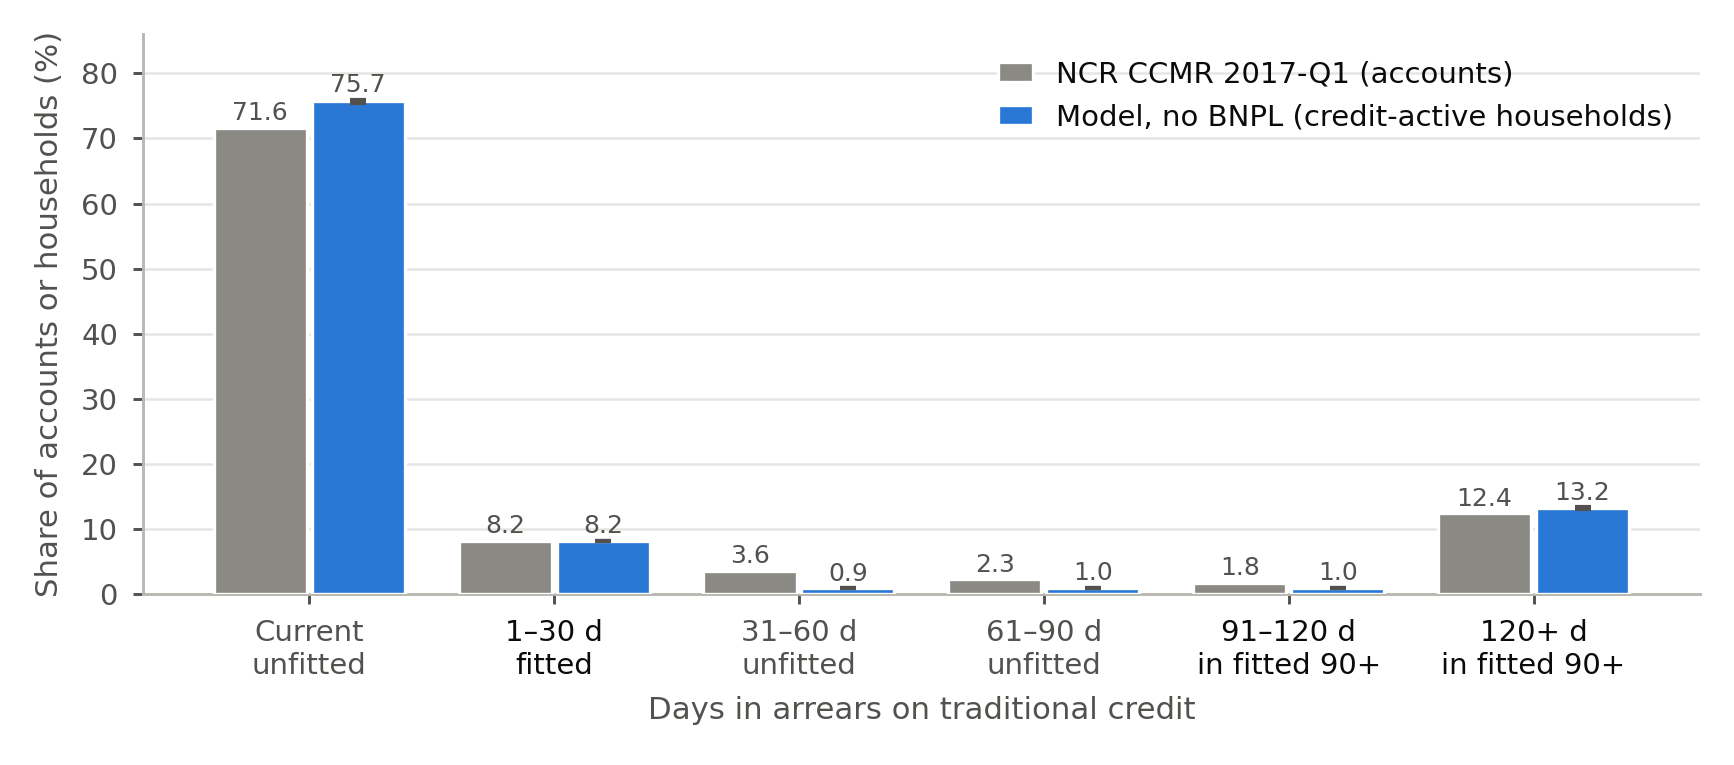
\includegraphics[width=\textwidth]{figures/fig_baseline_arrears.png}
\caption{The baseline arrears profile against the \ac{CCMR}}
\label{fig:baseline-arrears}
\tabnote{The distribution of credit-active households (those holding traditional debt or arrears) by days in arrears, with \ac{BNPL} disabled, against the \ac{CCMR}'s account-level age analysis for the first quarter of 2017 (Table~\ref{tab:ccmr}). Model bars are post-burn-in averages of each band, as means over 20 replicates of the baseline arm (seeds 10{,}000--10{,}019), with 95\% confidence intervals of the mean. Calibration fits the 1--30 day band and the combined 90+ share; the split between the 91--120 and 120+ day bands is not fitted. Table~\ref{tab:arrears-fit} reports the same profile from the calibration run. Because the \ac{CCMR} counts accounts and the model counts households, the comparison is of shape and scale.}
\end{figure}

% GENERATED by notebooks/scripts/build_results_tables.py from results/raw --
% do not edit by hand; re-run the script instead.
\begin{table}[H]
\centering
\caption{The 2017 baseline and the \ac{BNPL} injection}
\label{tab:baseline-arms}
\tabnote{The calibrated baseline with \ac{BNPL} disabled, and the same population with \ac{BNPL} enabled at four platforms and access at the banked ceiling, without ($\beta = 0$) and with ($\beta = 1$) peer influence. Means over 20 replicates, replicate standard deviation in brackets (seeds 10{,}000--10{,}019 in each arm). The default rate is the share of all households in default at the final tick; the 90+ day share is over credit-active households, averaged over post-burn-in ticks; the traditional arrears rate is the share of all households with a traditional instalment in arrears, averaged over post-burn-in ticks; interest, lending and volume are sums over the post-burn-in horizon in 2017 Rands. ``Holders'' are households with a positive \ac{BNPL} balance at the final tick; ``ever'' quantities are over every tick of the run, burn-in included. Default is absorbing, so the final-tick rate is the share of households that defaulted at any tick of the run. Default with \ac{BNPL} less default without: $+0.03 \pm 0.09$pp at $\beta = 0$ and $+0.61 \pm 0.11$pp at $\beta = 1$; the arms share seeds, so each difference is paired by seed and carries one standard error.}
\begingroup\setlength{\tabcolsep}{4pt}\footnotesize
\begin{tabular}{L{6.4cm}rrr}
\toprule
\textbf{Outcome} & \textbf{No \ac{BNPL}} & \textbf{\ac{BNPL}, $\beta=0$} & \textbf{\ac{BNPL}, $\beta=1$} \\
\midrule
Population default rate (\%) & 13.31 (0.32) & 13.34 (0.35) & 13.92 (0.28) \\
90+ day arrears, credit-active households (\%) & 14.20 (0.41) & 14.40 (0.43) & 14.60 (0.29) \\
Traditional arrears rate, all households (\%) & 10.64 (0.22) & 10.87 (0.22) & 11.21 (0.16) \\
Traditional interest charged (R m) & 13.01 (0.28) & 12.81 (0.17) & 12.97 (0.25) \\
New traditional lending granted (R m) & 6.12 (0.39) & 5.43 (0.32) & 6.11 (0.39) \\
Applications refused at the gate (count) & 1195 (28) & 1196 (24) & 1205 (24) \\
Zero liquid savings (\% of households) & 25.7 (0.2) & 25.9 (0.2) & 28.8 (0.2) \\
Holding \ac{BNPL}, end of horizon (\%) & 0.00 (0.00) & 17.55 (0.44) & 66.80 (0.40) \\
Ever held a \ac{BNPL} balance (\%) & 0.00 (0.00) & 69.97 (0.42) & 75.54 (0.15) \\
Balances on two or more platforms, end of horizon (\% of households) & 0.00 (0.00) & 9.12 (0.21) & 56.87 (0.57) \\
Balances on two or more platforms, end of horizon (\% of holders) & -- & 52.0 (0.7) & 85.1 (0.5) \\
Ever held balances on two or more platforms (\% of households) & 0.00 (0.00) & 25.78 (0.45) & 74.44 (0.17) \\
Ever held balances on two or more platforms (\% of those that ever held \ac{BNPL}) & 0.0 (0.0) & 36.8 (0.6) & 98.6 (0.2) \\
Cumulative \ac{BNPL} volume (R m) & 0.00 (0.00) & 6.42 (0.22) & 65.88 (0.91) \\
\bottomrule
\end{tabular}
\endgroup
\end{table}


\subsection{Stacking Across Platforms}
\label{sec:results-stacking}

Households come to owe several platforms at once, more so with more platforms and, under
random routing, with peer influence (Table~\ref{tab:stacking}; Figure~\ref{fig:stacking}).
With four platforms, 52.0\% of final-tick holders have balances on two or more platforms at
$\beta=0$, and 85.1\% at $\beta=1$ (Table~\ref{tab:baseline-arms}). These shares follow
from random routing (Section~\ref{sec:stacking}), under which a second request reaches a
different platform first with probability $3/4$ with four platforms and $5/6$ with six.

Under loyal routing the shares fall to 36.6\% at $\beta=0$ and 22.0\% at $\beta=1$, against
52.6\% and 85.2\% under random routing on the same seeds, and the share of ever-holders who
stacked at $\beta=1$ falls from 98.6\% to 51.4\%, nearer the \ac{CFPB}'s 32 and 33\%.
Default does not change detectably: $-0.07 \pm 0.07$ points at $\beta=0$ and
$+0.02 \pm 0.13$ at $\beta=1$ (seeds of Table~\ref{tab:effect}), although differences of
about 0.2 and 0.25 points cannot be excluded. How often households owe several platforms
depends on how they choose among platforms; default shows no detectable dependence.

Cumulative \ac{BNPL} volume rises when a second platform is added, from R5.14 million to
R6.16 million at $\beta=0$, and changes little from two platforms to six. This is consistent
with a second platform relieving limits that bind with one, and with further platforms adding
capacity that budget-based demand does not use. The sweep therefore cannot show what additional
platforms would do in a market where they expand borrowing.

Default does not change detectably with platform count. Going from one platform to six gives
$+0.02 \pm 0.09$ points at $\beta=0$ and $+0.01 \pm 0.08$ at $\beta=1$, and no contrast
between one platform and a larger number exceeds two standard errors at any $\beta$
(Table~\ref{tab:stacking-full}). Each platform brings its own limit, so platform count and
total credit capacity move together, and the sweep cannot separate the effect of platforms
not seeing one another from the effect of extra capacity.

% GENERATED by notebooks/scripts/build_results_tables.py from results/raw --
% do not edit by hand; re-run the script instead.
\begin{table}[H]
\centering
\caption{Cross-platform stacking and default by platform count}
\label{tab:stacking}
\tabnote{The platform-count sweep of the stacking experiment, at $\beta = 0$ (no peer influence, the control) and $\beta = 1$; the baseline is four platforms. ``2+'' is the share holding a balance on two or more platforms at the final tick, as a share of all households and of households holding any \ac{BNPL} balance at that tick; ``ever 2+'' is the share of households that ever held a \ac{BNPL} balance and at some tick held two or more, the nearest analogue of the \ac{CFPB}'s share of borrowers with simultaneous loans at more than one firm. With one platform the share is zero by construction. ``Volume'' is cumulative post-burn-in \ac{BNPL} volume in R million. Means over 20 replicates, replicate standard deviation in brackets for volume and default (seeds 20{,}000--20{,}019 in every cell); the three share columns are replicate means in per cent, with replicate standard deviations of at most 1.6 points. Every run uses the fitted shock probability 0.016 and payment friction 0.09 and access at the banked ceiling. Default at six platforms less default at one: $+0.02 \pm 0.09$pp at $\beta = 0$ and $+0.01 \pm 0.08$pp at $\beta = 1$; the arms share seeds, so each difference is taken seed by seed and carries one paired standard error, the standard deviation of the twenty differences over $\sqrt{20}$. The other three values of $\beta$ are in Table~\ref{tab:stacking-full}.}
\begingroup\setlength{\tabcolsep}{3pt}\scriptsize
\begin{tabular}{c rrrrr rrrrr}
\toprule
& \multicolumn{5}{c}{$\beta = 0$} & \multicolumn{5}{c}{$\beta = 1$} \\ \cmidrule(lr){2-6}\cmidrule(lr){7-11}
\textbf{Platforms} & \textbf{2+} & \textbf{holders} & \textbf{ever} & \textbf{Volume} & \textbf{Default (\%)} & \textbf{2+} & \textbf{holders} & \textbf{ever} & \textbf{Volume} & \textbf{Default (\%)} \\
\midrule
1 & 0.0 & 0.0 & 0.0 & 5.14 (0.18) & 13.33 (0.31) & 0.0 & 0.0 & 0.0 & 58.09 (0.60) & 13.86 (0.24) \\
2 & 8.5 & 48.1 & 33.2 & 6.16 (0.21) & 13.51 (0.29) & 46.8 & 70.1 & 98.4 & 64.89 (0.78) & 13.92 (0.30) \\
3 & 9.1 & 51.1 & 35.7 & 6.37 (0.28) & 13.37 (0.36) & 54.3 & 81.3 & 98.5 & 66.08 (0.77) & 13.78 (0.31) \\
4 & 9.2 & 52.4 & 36.8 & 6.41 (0.21) & 13.46 (0.29) & 56.7 & 85.0 & 98.6 & 66.30 (0.63) & 13.85 (0.32) \\
5 & 9.3 & 53.2 & 37.6 & 6.47 (0.31) & 13.44 (0.34) & 58.5 & 87.6 & 98.6 & 65.99 (1.08) & 13.85 (0.31) \\
6 & 9.4 & 53.6 & 37.9 & 6.39 (0.37) & 13.35 (0.29) & 59.2 & 88.6 & 98.5 & 66.09 (0.98) & 13.88 (0.27) \\
\bottomrule
\end{tabular}
\endgroup
\end{table}


\begin{figure}[H]
\centering
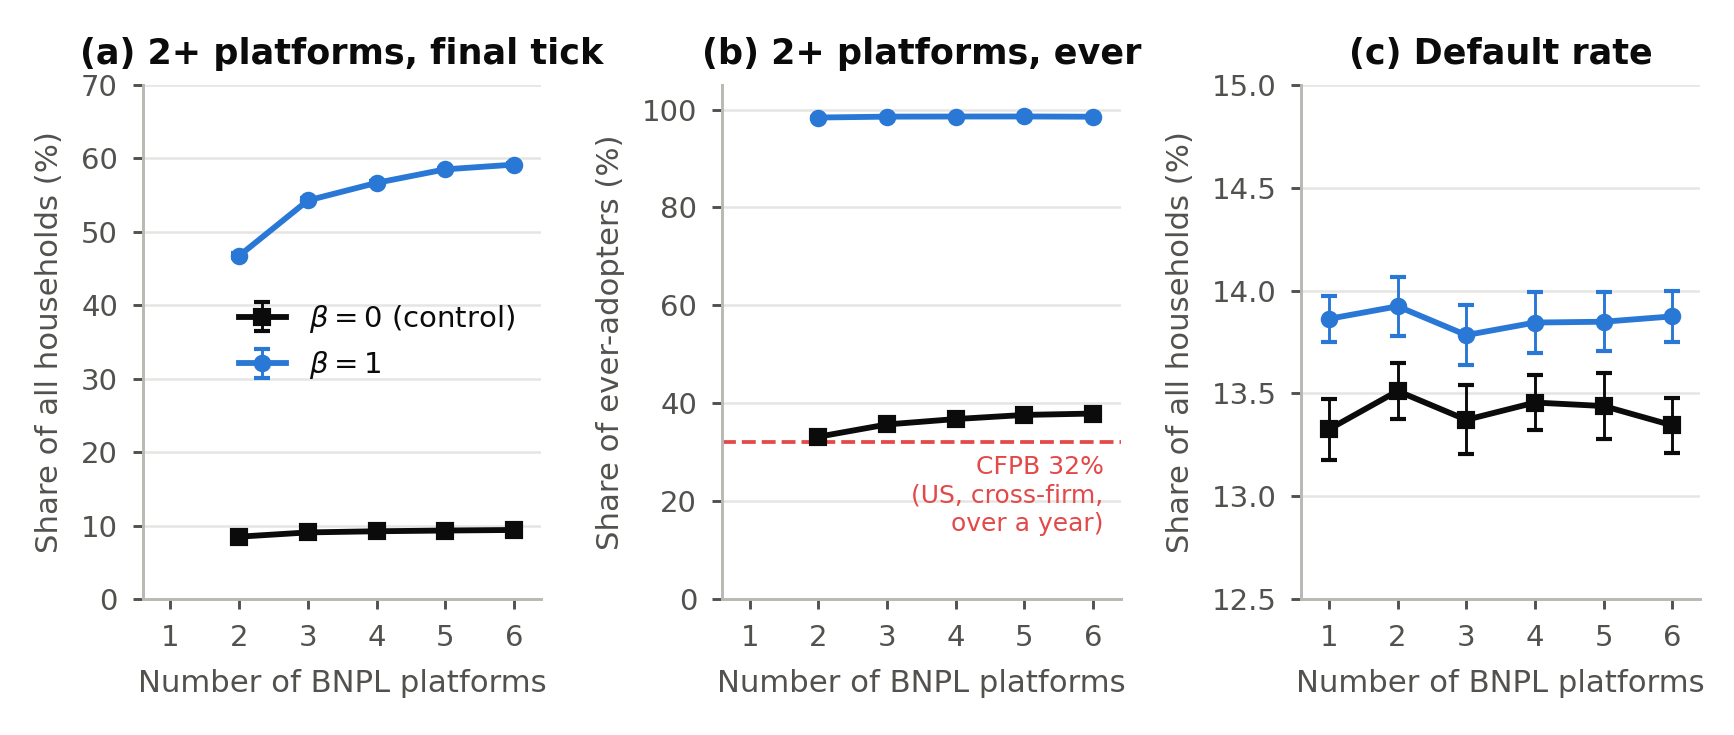
\includegraphics[width=\textwidth]{figures/fig_stacking.png}
\caption{Stacking and default by platform count}
\label{fig:stacking}
\tabnote{Panel (a): the share of all households holding balances on two or more platforms at the final tick. Panel (b): the share of households that ever held a \ac{BNPL} balance and at some tick held balances on two or more platforms, the nearest analogue of the \ac{CFPB}'s share of United States \ac{BNPL} borrowers with simultaneous loans at two or more firms during a year, 32\% in 2021 (dashed line) and 33\% in 2022; markets, units and observation periods differ. Both shares are zero by construction with one platform and are plotted from two. Panel (c): the population default rate. Series are $\beta = 0$ (black, the control) and $\beta = 1$; means over 20 replicates with 95\% confidence intervals of the mean; seeds and settings as in Table~\ref{tab:stacking}.}
\end{figure}

\subsection{BNPL Access, Peer Influence and Default}
\label{sec:results-rq2}

Default rises with access where peer influence is present (Figure~\ref{fig:access-default};
Table~\ref{tab:access}). At $\beta=0$, moving from zero to full access does not change
default detectably ($+0.14 \pm 0.11$ points). The rise grows with $\beta$, to
$0.60 \pm 0.11$ points at $\beta=1$ and $0.95 \pm 0.09$ at $\beta=3$.

The experiment cannot distinguish a straight line from a curved response. Steps between adjacent access
levels range from $-0.09$ to $+0.33$ points with standard errors of 0.07 to 0.14, and six of
the thirty exceed two standard errors. Under the linear rule, where the rise is detectable, straight-line fits to the arm means
have $R^2$ between 0.68 and 0.94.

The heterogeneous-threshold rule raises holding far more than the control does, but it does
not raise default detectably more. At
$\gamma=0.3$ the full-access share of households holding \ac{BNPL} rises by between 40.7 and
51.0 points, against 17.6 in the $\gamma=0$ control. Holding is close to linear in access
($R^2 \geq 0.998$), so no adoption cascade occurs on this grid. The rise in default
under the rule exceeds the rise in the control by between $0.05 \pm 0.08$ and
$0.14 \pm 0.13$ points, and none of these differences is detectable. Raising the mean
threshold from 0.15 to 0.45 lowers full-access holding from 50.8\% to 28.2\% but does not
change default detectably ($-0.17 \pm 0.11$ points).

\label{sec:no-cascade}
For default, the design cannot tell a line from a curve, so the absence of a tipping point
is not established. The lowest $R^2$ values
for default, 0.57 and 0.68, belong to small detectable rises, where replicate noise is
large beside the rise. The grid has seven access levels, so a threshold narrower than their
spacing could go undetected. No channel in the model carries one household's default to
another household's income or to a lender's supply of credit
(Table~\ref{tab:design-concepts}), so contagion through those channels lies outside the
test.

\begin{figure}[H]
\centering
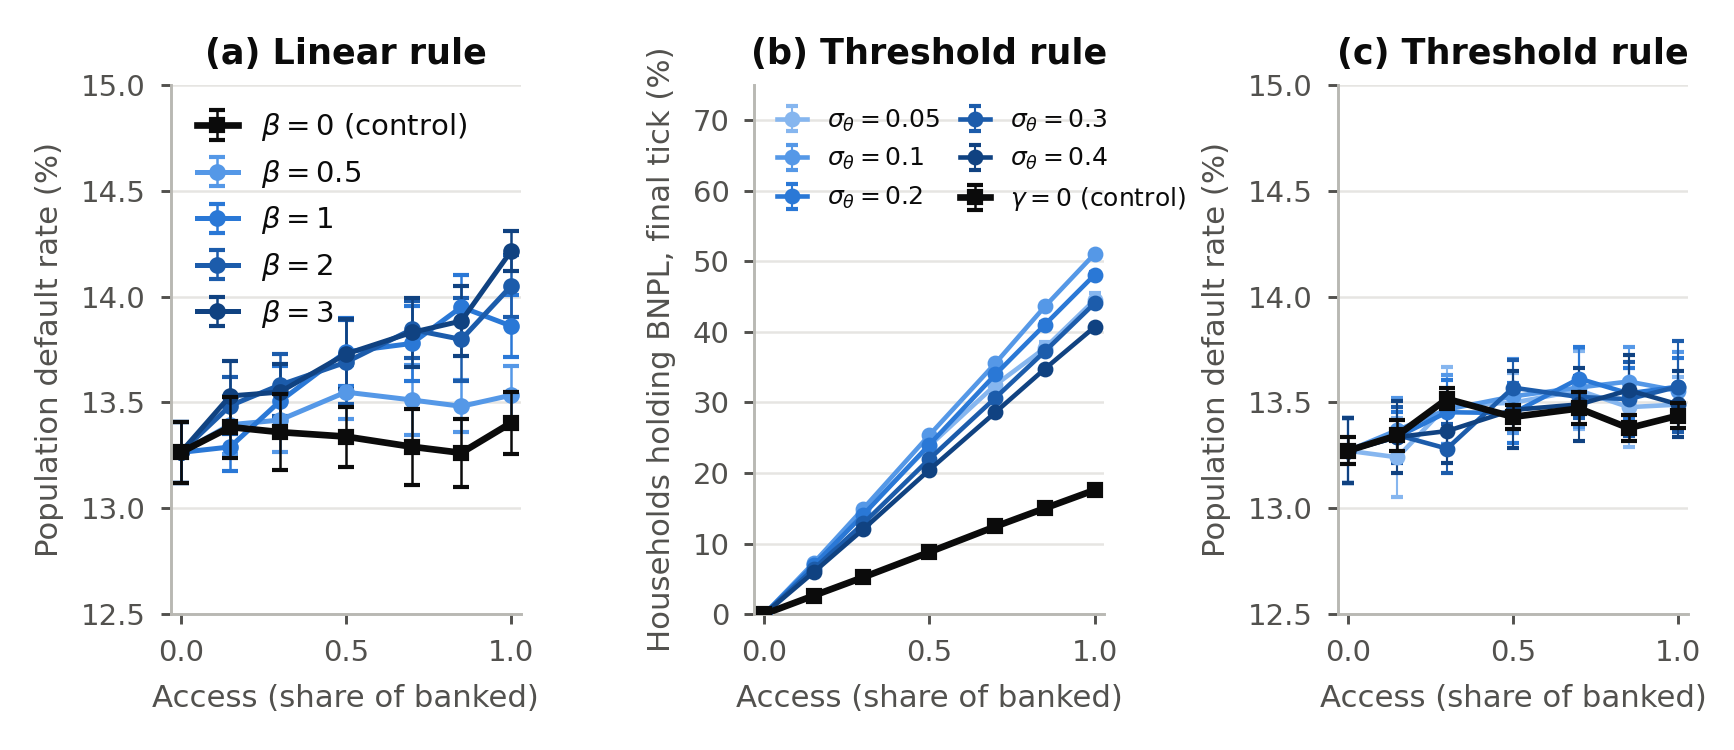
\includegraphics[width=\textwidth]{figures/fig_access_default.png}
\caption{Default against \ac{BNPL} access under two adoption rules}
\label{fig:access-default}
\tabnote{Panel (a): the population default rate at the final tick against \ac{BNPL} access, expressed as a share of the banked subpopulation (82.8\% of households), under the linear peer rule at each $\beta$ swept; the $\beta = 0$ control is black. Panels (b) and (c): the share of households holding \ac{BNPL} at the final tick, and the default rate, under the heterogeneous-threshold rule at each dispersion $\sigma_\theta$ with $\gamma = 0.3$; the $\gamma = 0$ control is black. Means over 20 replicates per point with 95\% confidence intervals of the mean; the end-to-end changes, fits and seeds are in Table~\ref{tab:access}.}
\end{figure}

% GENERATED by notebooks/scripts/build_results_tables.py from results/raw --
% do not edit by hand; re-run the script instead.
\begin{table}[H]
\centering
\caption{Response of default and holding to \ac{BNPL} access}
\label{tab:access}
\tabnote{Each row reports the change in the default rate from zero access to full access, over the seven access rates swept (0 to 1.0 of the banked subpopulation; the banked ceiling is 82.8\% of all households). The two end arms share seeds, so the change is paired by seed and carries one standard error. Where the change exceeds two standard errors the row also gives the $R^2$ of a straight line fitted to the seven arm means and the largest residual as a share of the change; a tipping point would show a low $R^2$ and a large residual. Where the change is within two standard errors there is no response to fit and the two cells are left empty. The holding column gives the same diagnostic for the share holding \ac{BNPL} at the final tick; it is computed for the threshold rule only. Linear-coupling cells have seeds 30{,}000--30{,}019, threshold cells 60{,}000--60{,}019 and the $\mu_\theta$ arms 61{,}000--61{,}019; 20 replicates each; every run uses the fitted shock probability 0.016 and payment friction 0.09, four platforms, and access at the banked ceiling unless stated. The $\gamma = 0$ control is identical at every $\sigma_\theta$ because thresholds are then never consulted.}
\begingroup\setlength{\tabcolsep}{4pt}\footnotesize
\begin{tabular}{L{3.7cm}rrrL{3.0cm}}
\toprule
\textbf{Arm} & \textbf{Default (pp)} & \textbf{$R^2$} & \textbf{Max residual} & \textbf{Holding} \\
\midrule
\multicolumn{5}{l}{\emph{Linear coupling, Equation~\ref{eq:peer} ($\beta$ swept)}} \\
$\beta = 0$ (control) & $+0.14 \pm 0.11$ & -- & -- & -- \\
$\beta = 0.5$ & $+0.27 \pm 0.11$ & 0.682 & 36.5\% & -- \\
$\beta = 1$ & $+0.60 \pm 0.11$ & 0.910 & 20.0\% & -- \\
$\beta = 2$ & $+0.78 \pm 0.09$ & 0.937 & 14.1\% & -- \\
$\beta = 3$ & $+0.95 \pm 0.09$ & 0.936 & 11.3\% & -- \\
\multicolumn{5}{l}{\emph{Heterogeneous thresholds ($\sigma_\theta$ swept, $\gamma = 0.3$; $\gamma = 0$ is the control)}} \\
$\gamma = 0$ (control) & $+0.17 \pm 0.10$ & -- & -- & +17.6pp, $R^2$ 1.000 \\
$\sigma_\theta = 0.05$ & $+0.22 \pm 0.09$ & 0.569 & 47.8\% & +44.5pp, $R^2$ 0.998 \\
$\sigma_\theta = 0.1$ & $+0.28 \pm 0.11$ & 0.829 & 25.6\% & +51.0pp, $R^2$ 1.000 \\
$\sigma_\theta = 0.2$ & $+0.30 \pm 0.10$ & 0.841 & 28.9\% & +48.1pp, $R^2$ 1.000 \\
$\sigma_\theta = 0.3$ & $+0.30 \pm 0.12$ & 0.742 & 42.6\% & +44.1pp, $R^2$ 1.000 \\
$\sigma_\theta = 0.4$ & $+0.22 \pm 0.10$ & 0.869 & 28.8\% & +40.7pp, $R^2$ 1.000 \\
\multicolumn{5}{l}{\emph{Threshold mean $\mu_\theta$ at full access, $\sigma_\theta = 0.20$, $\gamma = 0.3$}} \\
$\mu_\theta = 0.15$ & \multicolumn{3}{l}{default 13.57 (0.27)\%} & holding 50.8 (0.5)\% \\
$\mu_\theta = 0.3$ & \multicolumn{3}{l}{default 13.44 (0.34)\%} & holding 48.6 (0.9)\% \\
$\mu_\theta = 0.45$ & \multicolumn{3}{l}{default 13.40 (0.39)\%} & holding 28.2 (1.2)\% \\
\bottomrule
\end{tabular}
\endgroup
\end{table}


\subsection{Distribution Across Income Quintiles}
\label{sec:results-distribution}

Baseline default is highest in Q1 (17.83\%) and Q4 (15.75\%) and lowest in Q5 (10.10\%)
(Table~\ref{tab:distribution}). The same two quintiles have the highest aggregate
debt-to-income ratios (Pattern~3, Section~\ref{sec:data-validation}).

At $\beta=0$ enabling \ac{BNPL} changes default detectably in no quintile. At $\beta=1$ default
rises by $0.56 \pm 0.25$ points in Q2, $0.83 \pm 0.27$ in Q3 and $1.17 \pm 0.32$ in Q4, while
the changes in Q1 ($+0.03 \pm 0.22$) and Q5 ($+0.49 \pm 0.27$) are not detectable. The rise in
Q4 exceeds the rise in Q1 by $1.14 \pm 0.38$ points. At $\beta=0$ the
mean want-driven purchase rises from R103 in Q1 to R1{,}858 in Q5, as the budget-based sizing
rule implies. Larger purchases may explain why default rises more in Q4 than in Q1, but the
experiment does not test this, and Q5, with the largest purchases, shows no detectable rise.

The per-platform limit binds more often on poorer households, on 24.8\% of Q1 requests against
13.6\% in Q5, but loosening it matters little: raising $\lambda$
tenfold, from 0.10 to 1.0 months of income, changes population default by $+0.10 \pm 0.09$
points at $\beta=1$ (Table~\ref{tab:robustness-appendix}).

% GENERATED by notebooks/scripts/build_results_tables.py from results/raw --
% do not edit by hand; re-run the script instead.
\begin{table}[H]
\centering
\caption{Outcomes by income quintile}
\label{tab:distribution}
\tabnote{Each row is one per-capita income quintile of the 5{,}000-household population (the weighted \ac{NIDS} bounds of Appendix~\ref{app:variables}; quintile sizes 1{,}017, 987, 1{,}069, 937 and 990 households). Default is the share of the quintile's households in default at the final tick, in the no-\ac{BNPL} baseline and in the $\beta = 0$ arm of Table~\ref{tab:baseline-arms}; adoption and traditional arrears are final-tick shares of the quintile's households in the $\beta = 0$ arm, in per cent; debt-to-income is the aggregate ratio (total debt over total monthly income in the quintile) in the baseline; limit binding is the share of the quintile's \ac{BNPL} requests refused by the rolling per-platform limit, in per cent; the mean purchase is over the quintile's want-driven originations, in 2017 Rands. The default columns are means over 20 replicates, replicate standard deviation in brackets; the five right-hand columns are replicate means, with standard deviations of at most 2.6 points for the three shares, 0.04 for the ratio and R40 for the purchase. Every run uses the fitted shock probability 0.016 and payment friction 0.09, four platforms, and access at the banked ceiling unless stated. Default with \ac{BNPL} at $\beta = 0$ less default without: Q1 $-0.23 \pm 0.15$pp; Q2 $+0.11 \pm 0.27$pp; Q3 $+0.13 \pm 0.20$pp; Q4 $+0.22 \pm 0.29$pp; Q5 $-0.05 \pm 0.20$pp. At $\beta = 1$: Q1 $+0.03 \pm 0.22$pp; Q2 $+0.56 \pm 0.25$pp; Q3 $+0.83 \pm 0.27$pp; Q4 $+1.17 \pm 0.32$pp; Q5 $+0.49 \pm 0.27$pp. The arms share seeds, so each difference is taken seed by seed and carries one paired standard error, the standard deviation of the twenty differences over $\sqrt{20}$.}
\begingroup\setlength{\tabcolsep}{3pt}\scriptsize
\begin{tabular}{c rr r r r r r}
\toprule
& \multicolumn{2}{c}{Default rate (\%)} & & & & & \\ \cmidrule(lr){2-3}
\textbf{Quintile} & \textbf{No \ac{BNPL}} & \textbf{$\beta=0$} & \textbf{Adoption} & \textbf{Arrears} & \textbf{Debt/inc.} & \textbf{Limit binds} & \textbf{Purchase (R)} \\
\midrule
Q1 & 17.83 (0.64) & 17.61 (0.48) & 18.6 & 11.7 & 0.77 & 24.8 & 103 \\
Q2 & 10.84 (0.64) & 10.94 (0.97) & 15.6 & 12.7 & 0.36 & 23.3 & 157 \\
Q3 & 12.12 (0.88) & 12.25 (0.61) & 17.0 & 13.1 & 0.36 & 13.9 & 253 \\
Q4 & 15.75 (1.04) & 15.97 (1.33) & 19.4 & 15.1 & 0.69 & 13.8 & 411 \\
Q5 & 10.10 (0.73) & 10.05 (0.63) & 17.4 & 10.7 & 0.28 & 13.6 & 1{,}858 \\
\bottomrule
\end{tabular}
\endgroup
\end{table}


\subsection{Sensitivity and Robustness}
\label{sec:results-robustness}

Figure~\ref{fig:tornado} and Tables~\ref{tab:robustness} and~\ref{tab:robustness-appendix}
report the level of default in one-at-a-time sensitivity arms at $\beta=1$, four platforms and
full access. Each arm is compared with its group's reference arm, paired by seed except for
the population-size and single-tick shock arms. We use $\beta=1$ because the
\ac{BNPL}-side parameters have little to act on where households borrow little;
Table~\ref{tab:effect} reports the \ac{BNPL} effect under the same settings at both values
of $\beta$.

% Single-tick grid: results/summary/single_tick_calibration.json (notebooks/scripts/check_single_tick_calibration.py).
Shock persistence matters more than any other assumption. Replacing the persistent income
shock with a single-tick loss lowers default from 14.05\% to 4.81\%. Under that rule the
90+ share stays near 7.5\% at every shock probability on the calibration grid, with friction at 0.09, about half
the \ac{CCMR} target, so no shock probability on that grid restores the fit.

Among the behavioural rules, the largest influence on the default level is how much a
household borrows when short of cash (Submodel~4). Relative to borrowing the exact
shortfall, adding 25\% lowers default by $0.28 \pm 0.11$ points, and adding one tick of
committed expenditure lowers it by $1.02 \pm 0.13$. A plausible reason is that borrowing
beyond the immediate shortfall leaves a surplus in savings that absorbs later shortfalls,
but the experiment does not isolate this channel. No evidence places the true rule within
the range tested (Section~\ref{sec:amount}). Removing the shortfall cap, which limits
\ac{BNPL}'s share of a shortfall, does not change default detectably under any of the three
rules.

Three other assumptions move the default level. Shortening the default threshold from 98 to
56 days raises default by $0.84 \pm 0.11$ points. Varying $\kappa$ from 0.07 to 0.28, about
half to twice its derived value, moves default from 13.69\% to 14.34\%. Sizing purchases on
income in place of discretionary spending adds $0.68 \pm 0.11$ points. The other arms,
including the activation-order and population-size checks, change default by at most 0.35
points and none exceeds two standard errors (Table~\ref{tab:robustness-appendix}).

A Sobol decomposition over six parameters attributes the variance of the default level
almost entirely to the income-shock probability, sampled over 0.005--0.026, and gives each
\ac{BNPL}-side parameter a total-order index of about 0.01 (Table~\ref{tab:sobol}).

% GENERATED by notebooks/scripts/build_results_tables.py from results/raw --
% do not edit by hand; re-run the script instead.
\begin{table}[H]
\centering
\caption{Sensitivity of the default rate: principal arms}
\label{tab:robustness}
\tabnote{Population default rate at $\beta = 1$, four platforms and full access, for the principal sensitivity arms. Each group has its own reference arm at the default value, run on its own seed set (amount rules 50{,}000--50{,}019, default threshold 54{,}000--, $\kappa$ 57{,}000--, base 59{,}000--), so references differ from one another by seed noise only. Means over 20 replicates, replicate standard deviation in brackets. The difference column is arm less reference. Arms within a group share seeds, so the difference is paired by seed and carries one standard error. $\dagger$: uncapped less its capped twin, also paired. The shortfall rule and its cap have no literature anchor (Section~\ref{sec:amount}). The remaining arms are in Table~\ref{tab:robustness-appendix}.}
\begingroup\setlength{\tabcolsep}{4pt}\footnotesize
\begin{tabular}{L{7.2cm}rr}
\toprule
\textbf{Arm} & \textbf{Default (\%)} & \textbf{Difference (pp)} \\
\midrule
\multicolumn{3}{l}{\emph{Borrowing-amount rule (Submodel 4), \ac{BNPL} share of a shortfall capped}} \\
exact shortfall & 14.05 (0.47) & reference \\
shortfall $+25\%$ & 13.77 (0.30) & $-0.28 \pm 0.11$ \\
shortfall $+$ one tick of committed spending & 13.03 (0.40) & $-1.02 \pm 0.13$ \\
\multicolumn{3}{l}{\emph{The same rules with the cap removed (paired with the row above by seed)}} \\
exact shortfall, uncapped & 13.95 (0.29) & $-0.10 \pm 0.13^\dagger$ \\
shortfall $+25\%$, uncapped & 13.77 (0.27) & $-0.01 \pm 0.08^\dagger$ \\
shortfall $+$ one tick of committed spending, uncapped & 13.21 (0.43) & $+0.18 \pm 0.12^\dagger$ \\
\multicolumn{3}{l}{\emph{Default threshold $k$ (Submodel 7)}} \\
$k = 7$ ticks, 98 days & 14.00 (0.39) & reference \\
$k = 4$ ticks, 56 days & 14.84 (0.40) & $+0.84 \pm 0.11$ \\
\multicolumn{3}{l}{\emph{Purchase size $\kappa$ (Submodel 4)}} \\
$\kappa = 0.1387$ (IES-derived) & 13.86 (0.31) & reference \\
$\kappa = 0.07$ & 13.69 (0.33) & $-0.17 \pm 0.10$ \\
$\kappa = 0.28$ & 14.34 (0.34) & $+0.48 \pm 0.10$ \\
\multicolumn{3}{l}{\emph{Purchase sizing base (Submodel 4)}} \\
monthly discretionary budget & 13.78 (0.44) & reference \\
monthly income, $\kappa$ matched & 14.46 (0.21) & $+0.68 \pm 0.11$ \\
\bottomrule
\end{tabular}
\endgroup
\end{table}


\begin{figure}[H]
\centering
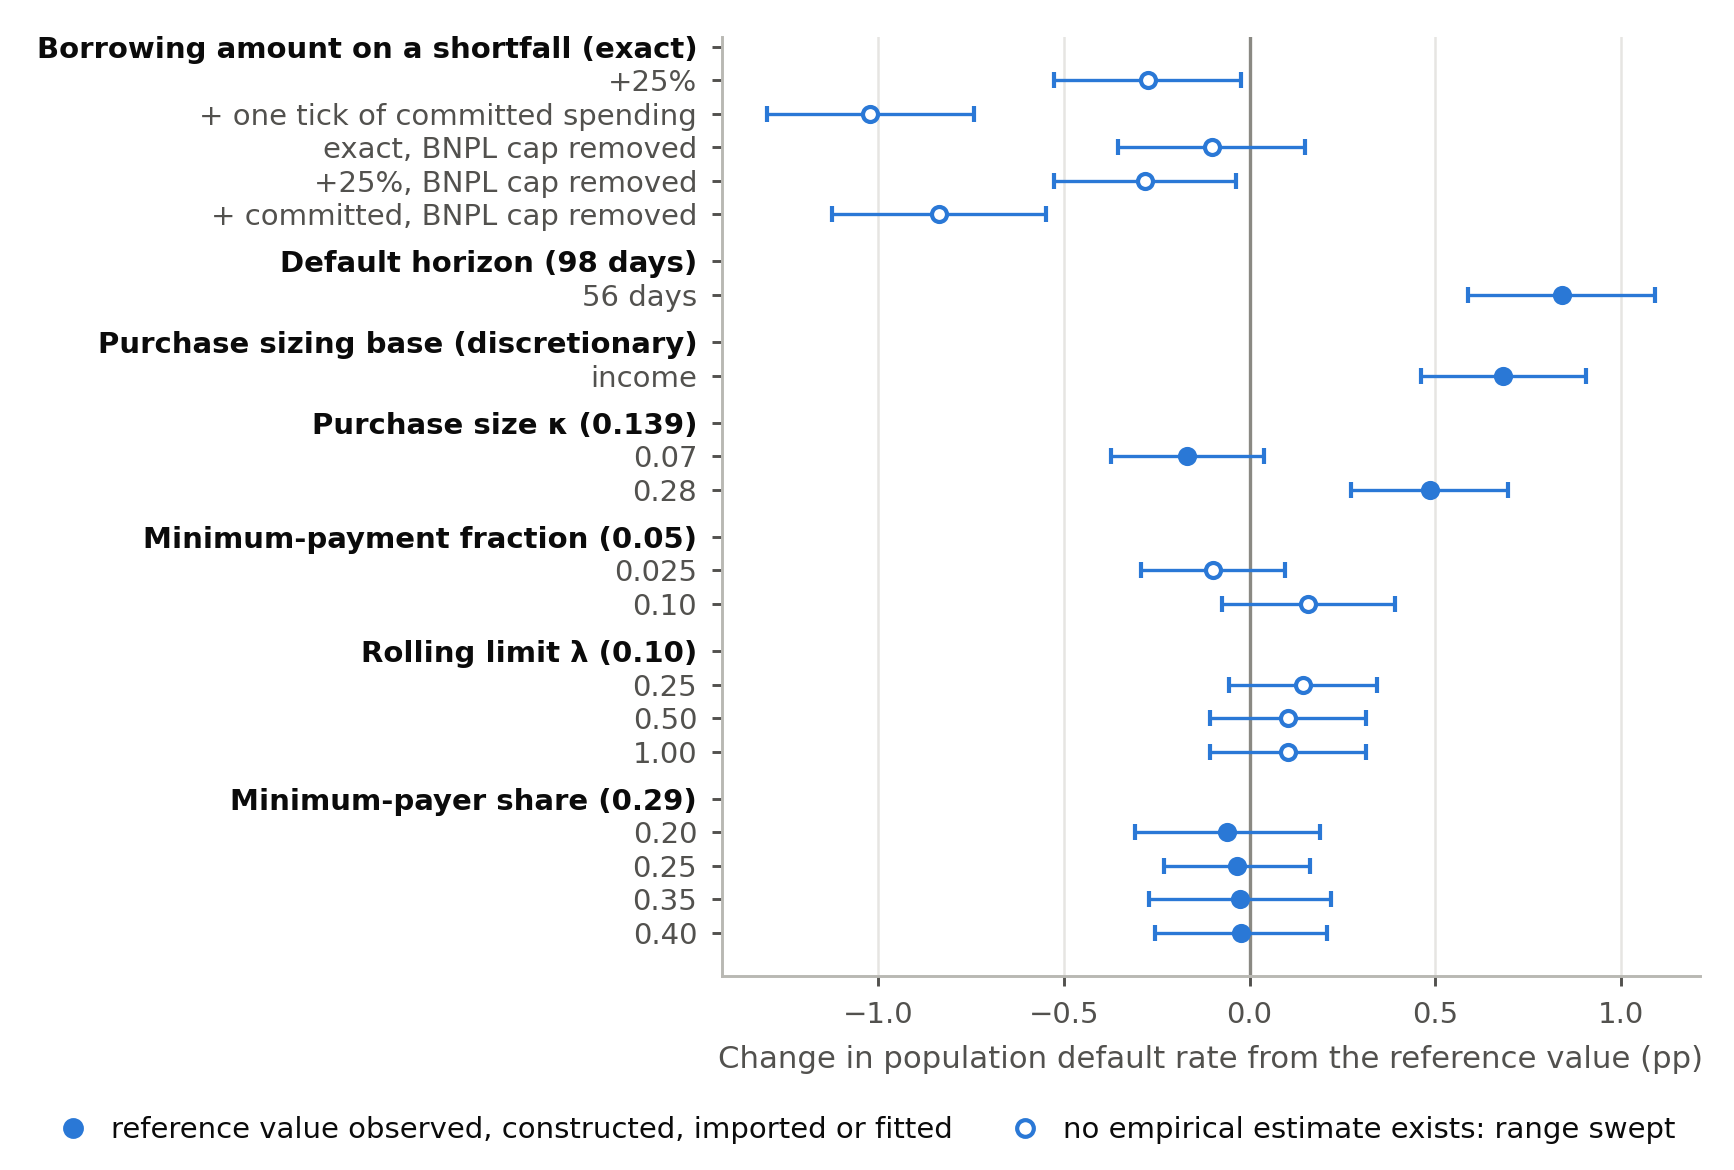
\includegraphics[width=\textwidth]{figures/fig_tornado.png}
\caption{Sensitivity of the population default rate}
\label{fig:tornado}
\tabnote{Each point is one sensitivity arm's change in the population default rate from its group's reference arm, at $\beta = 1$, four platforms and full access. Group headers, in bold, give the reference value. Bars are 95\% confidence intervals of the difference, paired by seed. The three cap-removed arms are compared with the exact-shortfall reference, whereas Table~\ref{tab:robustness} pairs each with its capped twin. Hollow markers identify rules and parameters for which no empirical estimate exists and whose range is swept (Table~\ref{tab:param-taxonomy}); filled markers have observed, constructed, imported or fitted reference values. The activation-order and population-size checks and the single-tick shock arm are in Table~\ref{tab:robustness-appendix}.}
\end{figure}

\subsubsection*{Robustness of the BNPL Effect}
\label{sec:results-effect}

The arms above measure the level of default with \ac{BNPL} enabled. Table~\ref{tab:effect}
tests the \ac{BNPL} effect itself. Every setting is run with \ac{BNPL} off and on, at
$\beta=0$ and $\beta=1$, over one shared seed block, so each effect is a paired difference on
the same seeds.

The settings share one seed block and often one no-\ac{BNPL} arm, so their results are
correlated, and counts of detectable settings are not independent replications.

At $\beta=1$ the effect is positive and detectable under nineteen of the twenty settings.
Among those nineteen it ranges from $0.25 \pm 0.09$ points at $\kappa=0.07$ to
$1.27 \pm 0.11$ where households borrow one tick of committed expenditure beyond the
shortfall and the shortfall cap is removed. Purchase size and the borrowing-amount rule move
it most: the effect is $0.91 \pm 0.07$ points at $\kappa=0.28$ and $1.22 \pm 0.10$ when
purchases are sized on income. Under the single-tick shock it is not detectable
($0.018 \pm 0.015$ points), with default without \ac{BNPL} at 4.82\%.

The three alternative rules for routing and the shortfall path leave the effect near its
reference value of $0.60 \pm 0.12$: $0.62 \pm 0.07$ under loyal routing, $0.68 \pm 0.11$
when credit pays a committed shortfall first, and $0.47 \pm 0.11$ when \ac{BNPL} cannot
relieve a shortfall at all. Most of the effect therefore runs through want-driven
borrowing.

At $\beta=0$ the effect ranges from $-0.11 \pm 0.08$ to $+0.52 \pm 0.09$ points. It exceeds
two standard errors under five of the twenty settings and is detectably negative under
none. Two of the five, $\lambda=0.25$ and $\lambda=1.0$, are one result: the limit seldom
binds at either value, so defaults are identical in every replicate. The largest value again
arises where households borrow beyond the shortfall with the shortfall cap removed.

{\renewcommand{\arraystretch}{0.94}% GENERATED by notebooks/scripts/build_results_tables.py from results/raw --
% do not edit by hand; re-run the script instead.
\begin{table}[H]
\centering
\caption{The \ac{BNPL} effect on default under each swept assumption}
\label{tab:effect}
\tabnote{The effect of enabling \ac{BNPL} on the population default rate at the final tick, under each setting of the sensitivity analysis, at $\beta = 0$ (the control) and $\beta = 1$. Each setting is run with \ac{BNPL} off and on over one seed block (70{,}000--70{,}019) shared by every arm, so each effect is a same-seed paired difference, \ac{BNPL} on less off, with one paired standard error. The no-\ac{BNPL} column gives the setting's own \ac{BNPL}-free default rate where the setting changes that model, and the reference arm's otherwise; means over 20 replicates, replicate standard deviation in brackets. Every run uses the fitted shock probability 0.016 and payment friction 0.09, four platforms, and access at the banked ceiling unless stated. The last row switches the want-driven path off, so \ac{BNPL} is used only to cover shortfalls.}
\begingroup\setlength{\tabcolsep}{4pt}\footnotesize
\begin{tabular}{L{4.8cm}rrr}
\toprule
\textbf{Setting} & \textbf{No \ac{BNPL} (\%)} & \textbf{Effect, $\beta=0$ (pp)} & \textbf{Effect, $\beta=1$ (pp)} \\
\midrule
\multicolumn{4}{l}{\emph{Reference}} \\
all parameters at default values & 13.30 (0.22) & $+0.15 \pm 0.07$ & $+0.60 \pm 0.12$ \\
\multicolumn{4}{l}{\emph{Borrowing amount on a shortfall (Submodel 4)}} \\
shortfall $+25\%$ & 13.14 (0.20) & $+0.12 \pm 0.09$ & $+0.72 \pm 0.08$ \\
shortfall $+$ one tick of committed spending & 12.02 (0.26) & $+0.22 \pm 0.10$ & $+1.08 \pm 0.11$ \\
exact shortfall, \ac{BNPL} cap removed & 13.30 (0.22) & $+0.05 \pm 0.09$ & $+0.59 \pm 0.09$ \\
shortfall $+25\%$, cap removed & 13.14 (0.20) & $-0.11 \pm 0.08$ & $+0.37 \pm 0.09$ \\
shortfall $+$ committed, cap removed & 12.02 (0.26) & $+0.52 \pm 0.09$ & $+1.27 \pm 0.11$ \\
\multicolumn{4}{l}{\emph{Default threshold (Submodel 7)}} \\
$k = 4$ ticks, 56 days & 14.24 (0.22) & $-0.01 \pm 0.06$ & $+0.76 \pm 0.11$ \\
\multicolumn{4}{l}{\emph{Minimum payments (Submodel 6)}} \\
minimum-payment fraction 0.025 & 13.16 (0.22) & $+0.06 \pm 0.10$ & $+0.50 \pm 0.09$ \\
minimum-payment fraction 0.10 & 13.42 (0.20) & $+0.06 \pm 0.10$ & $+0.70 \pm 0.09$ \\
minimum-payer share 0.20 & 13.35 (0.26) & $-0.05 \pm 0.09$ & $+0.54 \pm 0.11$ \\
minimum-payer share 0.40 & 13.34 (0.37) & $+0.24 \pm 0.14$ & $+0.65 \pm 0.12$ \\
\multicolumn{4}{l}{\emph{Purchase size and limits (Submodels 4 and 12)}} \\
$\kappa = 0.07$ & 13.30 (0.22) & $+0.01 \pm 0.10$ & $+0.25 \pm 0.09$ \\
$\kappa = 0.28$ & 13.30 (0.22) & $-0.02 \pm 0.09$ & $+0.91 \pm 0.07$ \\
purchases sized on income & 13.30 (0.22) & $+0.09 \pm 0.07$ & $+1.22 \pm 0.10$ \\
rolling limit $\lambda = 0.25$ & 13.30 (0.22) & $+0.20 \pm 0.07$ & $+0.63 \pm 0.11$ \\
rolling limit $\lambda = 1.0$ & 13.30 (0.22) & $+0.20 \pm 0.07$ & $+0.67 \pm 0.10$ \\
\multicolumn{4}{l}{\emph{Income-shock persistence (Submodel 1)}} \\
single-tick shock & 4.82 (0.06) & $-0.015 \pm 0.013$ & $+0.018 \pm 0.015$ \\
\multicolumn{4}{l}{\emph{Routing and the shortfall path (Submodels 5, 7 and 13)}} \\
platforms already owed tried first & 13.30 (0.22) & $+0.08 \pm 0.08$ & $+0.62 \pm 0.07$ \\
no \ac{BNPL} on the shortfall path & 13.30 (0.22) & $+0.06 \pm 0.10$ & $+0.47 \pm 0.11$ \\
credit pays a committed shortfall first & 13.31 (0.21) & $+0.06 \pm 0.09$ & $+0.68 \pm 0.11$ \\
\multicolumn{4}{l}{\emph{Want-driven path switched off ($q_{\text{base}} = 0$, $\beta = 0$)}} \\
\ac{BNPL} for shortfalls only & 13.30 (0.22) & $+0.05 \pm 0.09$ & -- \\
\bottomrule
\end{tabular}
\endgroup
\end{table}
}

\subsection{Answer to RQ2}
\label{sec:results-answer}

When platforms cannot observe one another, households come to owe several platforms at
once, more so with more platforms and, under random routing, with peer influence. With four
platforms and no peer influence, about half of final-tick holders owe two or more under
random routing and just over a third under loyal routing. These shares depend on the routing
rule; default does not change detectably with it, nor with platform count. Enabling
\ac{BNPL} raises default by $0.12 \pm 0.05$ points without peer influence, a result
sensitive to the borrowing rules, and by $0.60 \pm 0.07$ at $\beta=1$. Default rises with
peer influence and, where peer influence is present, with access: the arms in which
households borrow most. At $\beta=1$ the \ac{BNPL} effect is detectable in Q2 to Q4 but
not in Q1, the poorest quintile, or in Q5 (Table~\ref{tab:distribution}). No arm gives platforms a shared view of exposure,
so the experiments do not isolate the effect of platforms not seeing one another; mandatory
screening, which sees every platform's obligations, is examined in
Section~\ref{sec:scenarios}.

\section{Three Scenarios for the Lending Environment}
\label{sec:scenarios}

% Every number is read from thesis/chapters/generated/tab_scenarios.tex or tab_switches.tex
% (both from results/raw/rq3s.parquet, 100 replicates per arm), tab_cooloff.tex or tab_cap.tex,
% or from results/summary/results_numbers.json, all generated by
% notebooks/scripts/build_results_tables.py from results/raw. The exception is the agreements-cap
% diagnostic (32.9%, -0.11 +- 0.07), typed from results/corrections_2026-09-29/cap_definitions.md.

This section answers RQ3.
We compare three scenarios, the benchmark and two switches, with a fourth arm that combines the switches to test whether either changes the effect of the other.
The benchmark is the pre-2026 position, in which \ac{BNPL} obligations are invisible to the bureau and requests pass only a light screen.
The light screen in the benchmark is a modelling assumption; whether an agreement that levies late fees is incidental credit, and which provisions would then apply, is a legal question that the scenarios do not settle (Section~\ref{sec:background}).
Under bureau visibility ($\mathbb{1}^{\text{bur}}$), \ac{BNPL} obligations enter the traditional lender's Regulation 23A test. This is the affordability channel of the reported 2026 arrangements \cite{businessday_bnpl_2026}; the scoring channel is outside the model (Section~\ref{sec:asymmetry}).
Under mandatory affordability screening ($\mathbb{1}^{\text{aff}}$), the Regulation 23A test is applied to each \ac{BNPL} request, playing the role of the \ac{FCA}'s affordability check \cite{fca_ps26_1, woolard2021}.
Every arm is run at $\beta = 0$ and at $\beta = 1$ (Equation~\ref{eq:peer}), to test whether the results depend on peer influence.

Table~\ref{tab:scenarios} reports the outcomes, Table~\ref{tab:switches} sets the two switches beside their combination, and Figure~\ref{fig:scenarios} plots default and cumulative volume.
These four arms have one hundred replications each on shared seeds, five times the number used elsewhere, because the differences between them are small.
Differences are scenario less benchmark at the same $\beta$, taken seed by seed, and carry one standard error.
We report cumulative volume beside default because a rule that only delays borrowing within the horizon leaves volume unchanged, whereas a rule that prevents borrowing lowers it.

% GENERATED by notebooks/scripts/build_results_tables.py from results/raw --
% do not edit by hand; re-run the script instead.
\begin{table}[H]
\centering
\caption{Three scenarios for the lending environment, with and without peer influence}
\label{tab:scenarios}
\tabnote{The benchmark, bureau visibility and mandatory screening, as defined in Section~\ref{sec:scenarios}, each at $\beta = 0$ and $\beta = 1$. Bureau visibility covers the affordability channel only; the scoring channel is outside the model. Outcomes as in Table~\ref{tab:baseline-arms}; the by-quintile rows are the default rate within each per-capita income quintile of the population. Means over 20 replicates, replicate standard deviation in brackets; seeds 40{,}000--40{,}019 (benchmark), 41{,}000--41{,}019 (bureau) and 42{,}000--42{,}019 (screening); every run uses the fitted shock probability 0.016 and payment friction 0.09, four platforms, and access at the banked ceiling unless stated. Refusals are those of the traditional lender; a \ac{BNPL} request refused by the screening test is not counted there. Scenario less benchmark: the arms use different seed blocks, so each difference carries one unpaired standard error, $\sqrt{s_a^2/n_a + s_b^2/n_b}$ over the two arms' replicates: at $\beta = 0$, bureau visibility $+0.04 \pm 0.10$pp on default, $+0.14 \pm 0.13$pp on 90+ arrears and $-5.1 \pm 1.4\%$ on volume; screening $-0.02 \pm 0.10$pp on default, $-0.09 \pm 0.13$pp on 90+ arrears and $-5.3 \pm 1.3\%$ on volume; at $\beta = 1$, bureau visibility $+0.09 \pm 0.12$pp on default, $+0.19 \pm 0.13$pp on 90+ arrears and $-0.7 \pm 0.3\%$ on volume; screening $-0.09 \pm 0.13$pp on default, $-0.19 \pm 0.15$pp on 90+ arrears and $-1.5 \pm 0.3\%$ on volume.}
\begingroup\setlength{\tabcolsep}{2.5pt}\scriptsize
\begin{tabular}{L{3.5cm}rrrrrr}
\toprule
& \multicolumn{3}{c}{$\beta = 0$} & \multicolumn{3}{c}{$\beta = 1$} \\ \cmidrule(lr){2-4}\cmidrule(lr){5-7}
\textbf{Outcome} & \textbf{Benchmark} & \textbf{Bureau} & \textbf{Screening} & \textbf{Benchmark} & \textbf{Bureau} & \textbf{Screening} \\
\midrule
Population default rate (\%) & 13.41 (0.34) & 13.44 (0.32) & 13.39 (0.29) & 13.94 (0.35) & 14.03 (0.38) & 13.85 (0.44) \\
90+ day arrears, credit-active (\%) & 14.40 (0.46) & 14.54 (0.33) & 14.31 (0.34) & 14.65 (0.46) & 14.84 (0.36) & 14.46 (0.48) \\
Traditional arrears rate (\%) & 10.90 (0.26) & 10.96 (0.18) & 10.87 (0.21) & 11.23 (0.22) & 11.30 (0.21) & 11.16 (0.26) \\
Holding \ac{BNPL}, end of horizon (\%) & 17.64 (0.46) & 17.45 (0.47) & 15.74 (0.50) & 66.79 (0.36) & 66.58 (0.34) & 63.96 (0.37) \\
Cumulative \ac{BNPL} volume (R m) & 6.50 (0.27) & 6.17 (0.30) & 6.16 (0.24) & 66.00 (0.69) & 65.51 (0.71) & 65.02 (0.63) \\
New traditional lending granted (R m) & 5.46 (0.41) & 4.87 (0.32) & 5.33 (0.47) & 5.93 (0.35) & 5.37 (0.42) & 5.82 (0.29) \\
Traditional applications refused & 1191 (24) & 1395 (39) & 1202 (26) & 1207 (32) & 1415 (29) & 1192 (25) \\
Default rate, Q1 (\%) & 17.58 (0.61) & 18.12 (0.64) & 17.91 (0.50) & 17.96 (0.70) & 18.37 (0.59) & 17.83 (0.50) \\
Default rate, Q2 (\%) & 11.02 (0.65) & 10.96 (0.77) & 11.02 (0.78) & 11.15 (0.61) & 11.21 (0.74) & 11.11 (0.53) \\
Default rate, Q3 (\%) & 12.30 (0.65) & 12.32 (0.78) & 12.17 (0.77) & 13.01 (1.04) & 12.67 (0.94) & 12.74 (0.85) \\
Default rate, Q4 (\%) & 16.18 (0.91) & 15.82 (0.92) & 15.58 (1.04) & 16.79 (1.17) & 17.19 (0.82) & 16.66 (0.88) \\
Default rate, Q5 (\%) & 10.07 (0.92) & 10.08 (0.75) & 10.35 (0.84) & 10.89 (1.07) & 10.85 (0.85) & 11.03 (0.90) \\
\bottomrule
\end{tabular}
\endgroup
\end{table}


\begin{figure}[H]
\centering
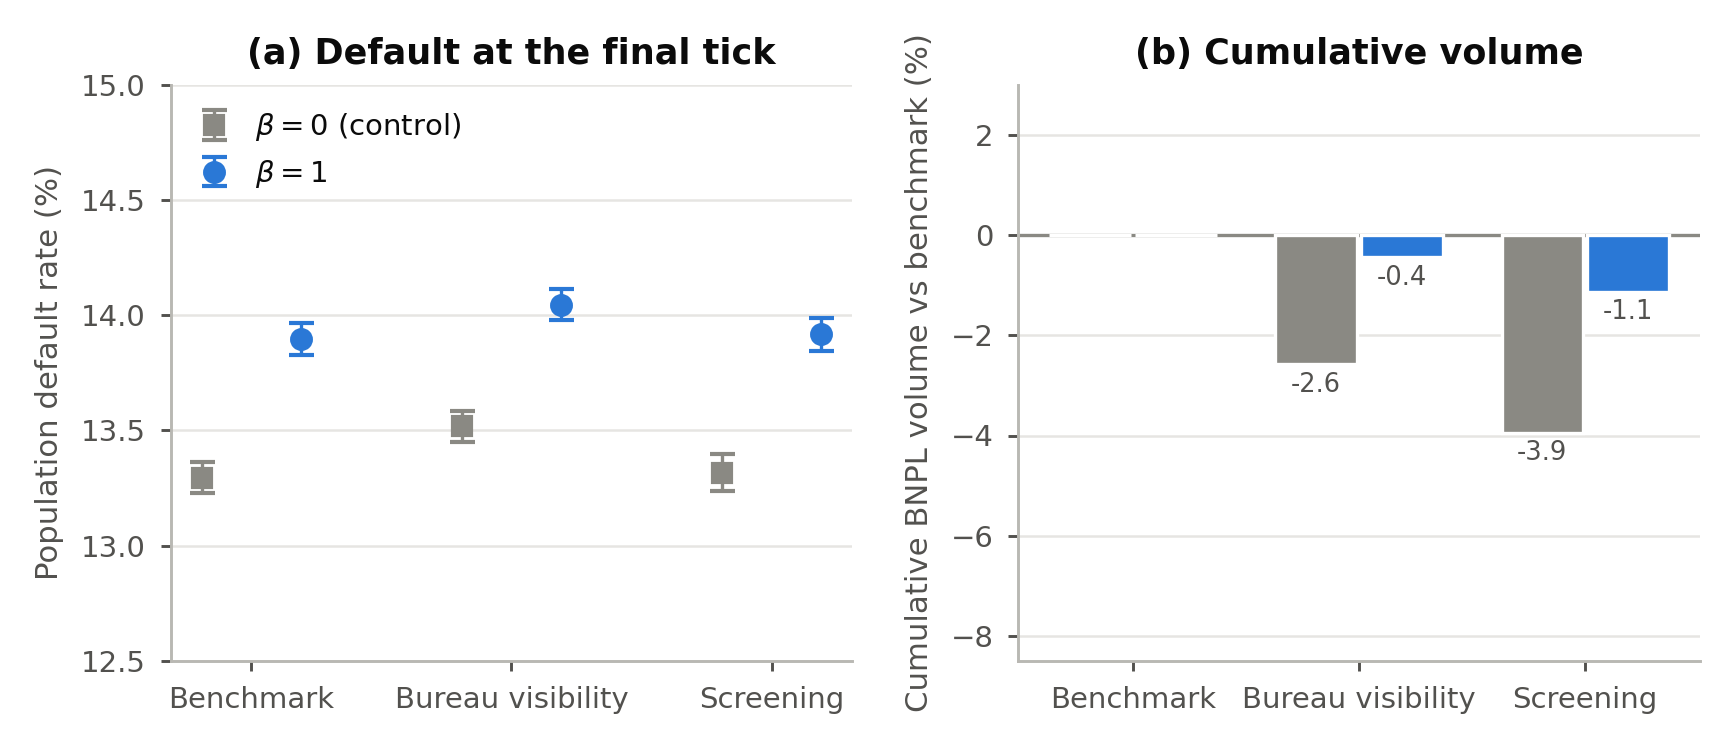
\includegraphics[width=\textwidth]{figures/fig_scenarios.png}
\caption{Default and cumulative volume under the three scenarios}
\label{fig:scenarios}
\tabnote{Panel (a): the population default rate at the final tick under the benchmark, bureau visibility and mandatory screening, at $\beta = 0$ (grey, the control) and $\beta = 1$; means over 100 replicates with 95\% confidence intervals of the mean. Panel (b): cumulative post-burn-in \ac{BNPL} volume relative to the benchmark at the same $\beta$. Seeds and definitions as in Table~\ref{tab:scenarios}; the two switches together, the cooling-off window and the hypothetical cap are in Tables~\ref{tab:switches}, \ref{tab:cooloff} and~\ref{tab:cap}.}
\end{figure}

% GENERATED by notebooks/scripts/build_results_tables.py from results/raw --
% do not edit by hand; re-run the script instead.
\begin{table}[H]
\centering
\caption{Bureau visibility and screening, alone and together}
\label{tab:switches}
\tabnote{Outcomes as in Table~\ref{tab:scenarios}, against the same benchmark arm. $\Delta$ is arm less benchmark on default, paired by seed with one standard error, since every arm shares the benchmark's seeds. ``Vol.'' is the change in cumulative post-burn-in \ac{BNPL} volume relative to the benchmark, in per cent: a rule that only delays borrowing within the horizon leaves it unchanged. ``Trad.'' is new traditional lending granted, in R million. Default, in per cent: means over 100 replicates, replicate standard deviation in brackets; holding at the final tick is a replicate mean in per cent with a standard deviation of at most 0.5 points. Every run uses the fitted shock probability 0.016 and payment friction 0.09, four platforms, and access at the banked ceiling unless stated. Seeds 80{,}000--80{,}099 in every arm. The screening test is shown the household's traditional service and its \ac{BNPL} instalments and arrears on every platform, whether or not the bureau switch is on; the bureau switch changes only what the traditional lender is shown.}
\begingroup\setlength{\tabcolsep}{1.5pt}\scriptsize
\begin{tabular}{L{1.9cm} rrrrr rrrrr}
\toprule
& \multicolumn{5}{c}{$\beta = 0$} & \multicolumn{5}{c}{$\beta = 1$} \\ \cmidrule(lr){2-6}\cmidrule(lr){7-11}
\textbf{Arm} & \textbf{Default} & \textbf{$\Delta$ (pp)} & \textbf{Hold.} & \textbf{Vol.} & \textbf{Trad.} & \textbf{Default} & \textbf{$\Delta$ (pp)} & \textbf{Hold.} & \textbf{Vol.} & \textbf{Trad.} \\
\midrule
benchmark & 13.30 (0.34) & -- & 17.5 & -- & 5.39 & 13.90 (0.35) & -- & 66.7 & -- & 5.90 \\
bureau visibility & 13.52 (0.34) & $+0.22 \pm 0.04$ & 17.5 & -2.6 & 4.97 & 14.05 (0.34) & $+0.15 \pm 0.04$ & 66.5 & -0.4 & 5.38 \\
screening & 13.32 (0.40) & $+0.02 \pm 0.05$ & 15.7 & -3.9 & 5.47 & 13.92 (0.36) & $+0.02 \pm 0.06$ & 64.1 & -1.1 & 5.93 \\
both switches & 13.40 (0.31) & $+0.10 \pm 0.05$ & 15.9 & -4.9 & 5.10 & 14.01 (0.36) & $+0.11 \pm 0.05$ & 64.2 & -1.5 & 5.53 \\
\bottomrule
\end{tabular}
\endgroup
\end{table}


Bureau visibility raises default, and screening does not change it detectably.
The rise is $0.22 \pm 0.04$ points at $\beta = 0$ and $0.15 \pm 0.04$ at $\beta = 1$; at $\beta = 0$ that is more than the $0.12 \pm 0.05$ by which enabling \ac{BNPL} raises default (Section~\ref{sec:results-injection}), although the two come from different seeds.
Screening changes it by $+0.02 \pm 0.05$ and $+0.02 \pm 0.06$ points.
With standard errors of 0.05 and 0.06 points, an effect of screening of about a tenth of a point in either direction cannot be ruled out.
With both switches default is $0.10 \pm 0.05$ and $0.11 \pm 0.05$ points above the benchmark, each just beyond two standard errors.

Bureau visibility changes only the traditional lender's test, so it acts through that lender's refusals.
Once \ac{BNPL} obligations enter the Regulation 23A test, the lender refuses more applications, 1{,}388 against 1{,}190 at $\beta = 0$, and grants R4.97 million in place of R5.39 million.
The 90+ day arrears share among credit-active households rises by $0.42 \pm 0.05$ points at $\beta = 0$ and by $0.28 \pm 0.04$ at $\beta = 1$.
The rise in default is largest in Q1, at $0.59 \pm 0.07$ and $0.46 \pm 0.08$ points, is not detectable in Q2 to Q4, and is $0.23 \pm 0.10$ and $0.22 \pm 0.11$ points in Q5, just beyond two standard errors.
A household that the lender refuses leaves its shortfall unpaid and is recorded as distressed (Section~\ref{sec:amount}), which is consistent with these rises, although the aggregates do not show that the refused households are the ones that default.
Cumulative \ac{BNPL} volume is $2.6 \pm 0.6$\% lower at $\beta = 0$, although the switch does not act on \ac{BNPL} requests.

A refused household has no other source of credit in the model, and the horizon is two years: a loan that is granted postpones distress, and its later cost may fall outside the horizon.
The result therefore gives the direction of the affordability channel over two years in the model, not a forecast of the reporting arrangements.

Screening lowers \ac{BNPL} holding and volume.
Holding at the final tick falls from 17.54\% to 15.69\% at $\beta = 0$ and from 66.74\% to 64.11\% at $\beta = 1$, and cumulative volume is $3.9 \pm 0.5$\% lower at $\beta = 0$ and $1.1 \pm 0.2$\% lower at $\beta = 1$.
The screening test already sees the household's \ac{BNPL} instalments and arrears on every platform (Section~\ref{sec:asymmetry}), so adding bureau visibility to screening gives the platforms no new information.
Bureau visibility then acts only on the traditional lender, and at $\beta = 0$ screening roughly halves its effect: with both switches the lender refuses 114 more applications than in the benchmark, against 198 under bureau visibility alone, and default is $0.12 \pm 0.04$ points below default under bureau visibility alone.
At $\beta = 1$ the two arms do not differ detectably.

Three features of the model may explain why screening alone does not change default.
A \ac{BNPL} agreement is small beside the room that the Regulation 23A test allows: each platform limits a household to a tenth of its monthly income and the mean want-driven purchase is R633, itself below the market figure (Section~\ref{sec:data-validation}), so the test refuses only households already close to its limit.
The test assesses affordability at origination on the household's surveyed income, whereas sustained distress in the model follows income shocks that arrive later and outlast the household's buffer (Section~\ref{sec:results-robustness}).
The traditional lender also stands behind the platforms: a shortfall request that screening refuses passes in full to the lender (Algorithm~\ref{alg:gate}), whereas one that the lender refuses under bureau visibility goes unmet.
None of these explanations is tested, because the outcomes do not follow the screened households.

Peer influence raises default by 0.53 to 0.61 points in every arm, and the comparisons give no evidence that it alters the effect of either switch: the effect of bureau visibility is $0.07 \pm 0.06$ points smaller at $\beta = 1$ than at $\beta = 0$, which is not detectable.

Appendix~\ref{app:levers} reports two further levers, each run at both values of $\beta$ with twenty replications: a cooling-off window of one to four ticks after a want-driven purchase (Table~\ref{tab:cooloff}), and a cap on the number of platforms a household may owe, which is hypothetical because no jurisdiction imposes one (Table~\ref{tab:cap}).
At $\beta = 0$ neither lever changes default detectably, although a cap of one removes 40.1\% of volume.
At $\beta = 1$ every window and caps of one and two lower default by between $0.28 \pm 0.08$ and $0.39 \pm 0.12$ points, and remove between 31.8\% and 76.3\% of volume; a cap of three does not change default detectably.
At $\beta = 1$, a cap of two that counts agreements in place of platforms removes 32.9\% of volume and changes default by $-0.11 \pm 0.07$ points, against $-0.35 \pm 0.09$ for the cap as modelled on the same seeds (Appendix~\ref{app:levers}), so the experiments do not show that lost volume is what lowers default.
No lever was run under the alternative borrowing rules of Table~\ref{tab:effect} (Section~\ref{sec:amount}), and the model has no measure of what a household loses when a purchase or a shortfall loan is refused.

In answer to RQ3, bureau visibility leads the traditional lender to refuse more applications and raises default by 0.15 to 0.22 points, mostly in the lowest income quintile.
Mandatory screening lowers \ac{BNPL} holding and volume and on its own does not change default detectably; added to bureau visibility at $\beta = 0$, it lowers default by $0.12 \pm 0.04$ points relative to bureau visibility alone.

\section{Conclusion}
\label{sec:conclusion}

% Every number is read from the generated tables of Sections 3.5, 4 and 5 or from
% results/summary/results_numbers.json; nothing is typed.

This thesis asked how a lending channel outside the affordability and reporting regime affects a household population already in credit distress, and what bringing that channel inside the regime would change.
We answered with a controlled counterfactual under 2017 conditions, so the results describe mechanisms in the model and do not forecast South African default after 2017.

The answer to RQ1 is partial.
The model reproduces its two fitted arrears bands and passes three of four external checks on the population under broad tolerances, but it misses the intermediate arrears bands, the servicing share, the size and volume of \ac{BNPL} purchases, the interest measure of the complementarity pattern and the debt-to-income pattern (Tables~\ref{tab:validation} and~\ref{tab:bnpl-on-checks}).
It therefore supports comparisons between mechanisms better than statements about levels.

For RQ2, households come to owe several platforms at once: with four platforms and no peer influence, 52.0\% of final-tick holders owe two or more, a share set by the assumption that households choose among platforms at random.
Default does not change detectably with the number of platforms (Table~\ref{tab:stacking}).
Enabling \ac{BNPL} raises default by $0.12 \pm 0.05$ points without peer influence and by $0.61 \pm 0.11$ points at $\beta = 1$, in a market that borrows ten times as much (Table~\ref{tab:baseline-arms}), and default rises with access where peer influence is present (Table~\ref{tab:access}).

For RQ3, neither bureau visibility nor mandatory screening changes default detectably, alone or together, and the design cannot reliably detect a change of 0.25 points or less (Table~\ref{tab:switches}).
Both switches change lending: bureau visibility raises the traditional lender's refusals by about a sixth, and screening lowers \ac{BNPL} holding by 1.9 to 2.8 points.

Taken together, the results link the effect of \ac{BNPL} on default to the volume of borrowing.
Default rises where peer influence makes households borrow heavily, while the number of platforms a household owes makes no detectable difference.
Showing \ac{BNPL} obligations to an affordability test changes who receives credit but not, detectably, how many households default.
A plausible reason, which the experiments do not test, is that a test applied when credit is granted cannot anticipate the income shocks that drive sustained distress in the model.
The two levers that did lower default, a cooling-off window and a cap on platforms owed, did so only under peer influence and while removing a third or more of \ac{BNPL} volume.

The thesis makes three contributions.
The most secure is a household population that combines \ac{NIDS} financial data with imputed \ac{FinScope} inclusion flags and is checked against sources its construction did not use.
The second is a model in which two classes of lender differ in what they can observe, so that the gap in visibility can be switched on and off.
The third is a set of reproducible comparisons of access, adoption rules and lending restrictions.

\label{sec:lim-reading}
Three limits govern how these results should be read.
First, the level of default rests on two fitted parameters and on a borrowing-amount rule with no empirical estimate, which moves default by up to 1.02 points (Table~\ref{tab:robustness}), and on the persistence of income shocks: replacing the persistent shock with a single-tick loss lowers default by 9.23 points (Table~\ref{tab:robustness-appendix}).
Second, the bureau experiment adds \ac{BNPL} obligations to the traditional lender's affordability calculation and excludes credit scores, pricing and lenders' responses, so the scoring channel of the reporting arrangements is untested.
Third, the standard errors measure variation between replicates and exclude uncertainty in the inputs and in the model's structure.
Appendix~\ref{app:caveats} indexes every limitation recorded in the thesis.

\label{sec:future-work}
Four extensions follow from these results.

\textbf{Borrowing for a shortfall.} Evidence on how much households borrow against a shortfall, and from which lender, would replace the assumed borrowing rules, under which the \ac{BNPL} effect at $\beta = 1$ ranges from $0.37 \pm 0.09$ to $1.27 \pm 0.11$ points (Section~\ref{sec:amount}; Table~\ref{tab:effect}).

\textbf{Credit scoring.} A rule linking reported \ac{BNPL} behaviour to scores, pricing and refusals would test the channel that the reporting arrangements most directly open (Section~\ref{sec:asymmetry}).

\textbf{South African behavioural evidence.} Local estimates of minimum-payment behaviour, present bias, provider choice and the persistence of income shocks would replace the assumed and imported rules on which the outcome levels depend (Section~\ref{sec:lim-transfer}).

\textbf{Feedback and contagion.} A lender that restricts credit after losses, or a link from aggregate default to employment, would let distress spread through channels now excluded (Table~\ref{tab:design-concepts}).


% ============================================================================
% BACK MATTER
% ============================================================================

\bibliographystyle{plainurl}
\bibliography{main}

\appendix
\section{Design Rationale: Alternatives Considered and Rejected}
\label{app:rationale}

Section~\ref{sec:model} states the rules the model uses. This appendix records the alternatives
we considered and rejected, and why.

\subsection{Population Construction}

\textbf{Statistical fusion of \ac{NIDS} and \ac{FinScope}.} A hot-deck or model-based fusion would
recover finer joint structure between the two instruments than copying flags within an
income-quintile-by-province cell. It would bring its own validation burden and a real risk of
fitting the idiosyncrasies of two surveys rather than the population behind them. The simpler
match reproduces the cell marginals that the model needs (Appendix~\ref{app:matching}).

\textbf{\ac{CPI} forwarding to 2022.} An earlier design forwarded \ac{NIDS} monetary values to
2022, which required a second reference year, assumptions about how relative incomes moved between
the two, and 2022-vintage validation targets. Working entirely in 2017 Rands removes all three, and
the 2017 anchor is independently required by the counterfactual injection design.

\subsection{Household Decision Rules}

\textbf{A propensity-to-consume or buffer-stock consumption rule (Submodel~2).} Both require a
calibrated propensity for which no South African estimate exists, and both discard the
committed-versus-discretionary expenditure split already observed in the survey data.

\textbf{Cost ranking as the lender-choice rule (Submodel~5).} \ac{BNPL} is nominally interest-free,
so a cost-minimising rule selects it trivially and attributes the choice to price. Experimental
evidence links the choice to expected peer approval as well \cite{ackert2025bnpl}, and the two
mechanisms suggest different interventions: a price-driven choice should respond to disclosure
of effective cost, while a norm-driven one may not.

\textbf{Scheduled amortisation as the sole repayment rule (Submodel~6).} Keys and Wang
\cite{Keys2019} find that 29\% of credit-card accounts pay at or near the contractual minimum, and
that 9 to 20\% of accounts respond to changes in the minimum-payment formula in ways liquidity
constraints alone cannot explain, a lower bound on anchoring. A uniform amortisation rule would
suppress the behaviour by which obligations persist and compound.

\textbf{A debt-service-to-income threshold as the default condition (Submodel~7).} Any such
threshold is arbitrary, and the \ac{NCA} prescribes none. We use Madeira's cash-flow test
instead, which is consistent with the affordability rule the model already implements and
which Madeira compares with observed default rates in a middle-income economy
\cite{madeira2018chile}.

\textbf{A continuous present-bias parameter (Submodel~8).} No South African distribution exists
against which to calibrate one, so it would add an unconstrained free parameter. The model
carries a single binary behavioural type instead, whose share is sourced and swept.

\subsection{Lender and Platform Rules}

\textbf{A flat \ac{DSTI} cap as the credit-granting gate (Submodel~9).} An earlier version of this
model used a ceiling of 0.65. It was unsourced, the \ac{NCA} prescribes no such ratio, and it was
far too permissive at the bottom of the distribution: a 65\% rule would permit a household earning
R900 per month to service R585 per month. The Regulation 23A residual-income test produces a
ceiling that varies with income and spans zero to 93.2\% of income across the population.

\textbf{Making the \ac{BNPL} eligibility screen a full affordability test (Submodel~12).} The
asymmetry between the Regulation 23A test that binds registered lenders and the light screen that
\ac{BNPL} providers apply is the mechanism under study. Imposing a full affordability test on
\ac{BNPL} is an intervention, and appears as the screening scenario of Submodel~15.

\textbf{A purely multiplicative peer-influence rule (Submodel~11).} Every household opens with no
\ac{BNPL} balance, so the reference-group adoption share is identically zero at initialisation and
adoption could never begin. The additive form of Equation~\ref{eq:peer} gives $q_{\text{base}}$ and
$\beta$ the roles that $p$ and $q$ play in Bass diffusion.

\subsection{Environment and Scheduling}

\textbf{Macroeconomic dynamics (Submodel~16).} The environment is held fixed to isolate the
effect of introducing \ac{BNPL} under baseline conditions. A common macroeconomic shock could
be added to both arms, but would require a broader experimental design.

\textbf{A fixed activation order (Submodel~17).} A fixed order would let the same households
act first in every tick. Random activation avoids this, although little depends on it: there is
no shared credit pool for early households to exhaust, and all households read the same lagged
peer signal. Because Comer and Loerch \cite{comer2013activation} and Alizadeh and
Cioffi-Revilla \cite{alizadeh2015activation} find activation regimes can matter, the fixed
order is retained as a robustness arm (Appendix~\ref{app:activation}).

\section{Model Specification: Design Concepts and Parameter Register}
\label{app:specification}

\subsection*{B.1 Design concepts and exclusions}

Table~\ref{tab:design-concepts} gives the model's treatment of the eleven \ac{ODD} design concepts and the eight mechanisms it excludes by design.

\begin{longtable}{L{2.9cm}L{7.3cm}L{3.2cm}}
\caption{\ac{ODD} design concepts and design exclusions}
\label{tab:design-concepts} \\
\multicolumn{3}{p{13.4cm}}{\footnotesize The eleven design concepts of the \ac{ODD} protocol \cite{grimm2020odd}, each with the model's treatment and the literature that grounds it; ``None'' in the source column marks a modelling choice with no external anchor. The final row lists the eight mechanisms excluded by design and the reason for each. The absence of default-to-income and lender-loss feedback limits the contagion mechanisms tested in Section~\ref{sec:results-rq2}.} \\
\toprule
\textbf{Concept} & \textbf{Treatment} & \textbf{Source} \\
\midrule
\endfirsthead
\toprule
\textbf{Concept} & \textbf{Treatment} & \textbf{Source} \\
\midrule
\endhead
\bottomrule
\endfoot
Basic principles & Balance sheets form the accounting core. Heuristic decision rules replace intertemporal optimisation. Statutory regulations act as explicit computational gates. & \cite{cardaci2018inequality, dorazio2017micro, meier2010present, Keys2019, yun2020housing} \\
\addlinespace
Emergence & Default rates and adoption paths follow from household decisions; stacking depths follow from the routing rule of Submodel~13. Borrowing to service existing debt raises future obligations, while lagged peer adoption raises borrowing propensities. Setting $\beta=0$ removes the peer-adoption effect. & None \\
\addlinespace
Adaptation & Households compress discretionary spending and borrow against shortfalls from current liquidity, and their want-driven purchase propensity rises with lagged peer adoption; they form none of the income expectations that D'Orazio and Giulioni give their households. The traditional lender and the platforms are non-adaptive. & \cite{dorazio2017micro} \\
\addlinespace
Objectives & No forward-looking utility. Households satisfy obligations in a fixed priority order, compressing discretionary spending under stress. & \cite{meier2010present} \\
\addlinespace
Learning & Excluded. Behavioural rules are static over the horizon. & None \\
\addlinespace
Prediction & Excluded. Agents treat current income as persistent. & None \\
\addlinespace
Sensing & Agents know their own balance sheets and observe the lagged adoption share among their reference group's \ac{BNPL}-eligible members. In the benchmark the traditional lender sees only bureau-recorded traditional debt and defaults, and each platform sees only its own exposure; the bureau switch adds \ac{BNPL} obligations to the lender's view (Submodel~15). & \cite{nortonrose_bnpl_sa} \\
\addlinespace
Interaction & Households interact with lenders through credit applications, and with each other indirectly through reference-group adoption shares. & \cite{ackert2025bnpl} \\
\pagebreak
Stochasticity & Income shocks and re-employment, archetype and eligibility assignment, want-driven purchases and their size, platform routing order, payment friction, activation order, and threshold endowments (drawn from a separate stream so control arms reproduce exactly across threshold dispersion). Runs are seeded and replicated, with dispersion reported. & None \\
\addlinespace
Collectives & Reference groups (income quintile $\times$ province) aggregate individual adoption into the peer signal. & \cite{cardaci2018inequality} \\
\addlinespace
Observation & Tracked per tick: population default rate; the \ac{CCMR} arrears distribution of credit-active households; traditional debt, arrears and interest; \ac{BNPL} balances, holding, volume and fees; the number of platforms each household owes; reference-group adoption shares; and the share with no liquid savings. Per run: the traditional lender's applications, grants and refusals, order-cap and limit binding rates, and default, purchase size and debt-to-income by income quintile. & None \\
\addlinespace
Exclusions & Eight mechanisms are excluded by design. \emph{No macroeconomic dynamics}: holding the environment fixed isolates the injection effect under baseline conditions. \emph{No contagion}: one aggregate lender with no balance sheet that can fail, and no feedback from household default to income, so default cannot spread through these channels. \emph{No competition among traditional lenders}, which suppresses the lender-conduct mechanism of Hamill et al. \emph{No learning and no scarring}. \emph{No peer effects on consumption}: peer influence acts only on \ac{BNPL} adoption. \emph{Static household composition}. \emph{No credit scores or risk pricing}: the bureau switch acts only through the affordability test. \emph{No other source of credit}: a household that the lender refuses has no informal or alternative lender. & \cite{hamill2023creditcard, cardaci2018inequality} \\
\end{longtable}

\subsection*{B.2 Parameter register}

Table~\ref{tab:param-register} gives every parameter with its value, provenance and sweep range.
It is generated from the parameter declarations in \texttt{simulation/config.py} by
\texttt{notebooks/scripts/generate\_param\_register.py}.

Four groups of entries carry standing flags:
\begin{itemize}
    \item \textbf{The two fitted parameters.} The income-shock probability (Submodel~1) and the
    payment-friction rate (Submodel~6) are fitted to the \ac{CCMR} 90+ and 1--30 day bands, which
    is what makes the baseline calibrated rather than validated
    (Section~\ref{sec:lim-calibration}).
    \item \textbf{The uncited rules.} The shortfall borrowing amount (Submodel~4), \ac{BNPL} relief
    of a shortfall and its cap (Submodel~5), the minimum-payment fraction (Submodel~6), the use of
    credit raised against a committed shortfall (Submodel~7) and platform routing (Submodel~13)
    have no literature anchor. Each is varied in at least one arm. Three assumptions are not
    varied: purchase-size dispersion, the order cap, which binds on 0.3\% of platform requests
    at $\beta=0$, and the payment of \ac{BNPL} instalments before traditional debt
    (Section~\ref{sec:sequence}).
    \item \textbf{The uncalibrated peer coefficients.} $q_{\text{base}}$, $\beta$ and the
    threshold parameters of Submodel~11 have no South African estimate. The
    $\beta = 0$ and $\gamma = 0$ control arms are reported beside every peer-influence result;
    the level-sensitivity arms run at $\beta = 1$ only.
    \item \textbf{The rolling limit.} No South African provider publishes a limit. $\lambda = 0.10$
    is set so that four platform limits sum to about Woolard's illustrative \pounds1{,}000 of
    credit amassed across several lenders \cite{woolard2021}, 39\% of United Kingdom median
    monthly household disposable income, equivalised, in the year to March 2020
    \cite{ons_income_fye2020}. It is swept 0.10--1.0 and reported against a 0.10--0.48 band
    whose upper end expresses Afterpay's maximum of A\$2{,}000 as a share of Australian median
    monthly household disposable income, equivalised, in 2019--20
    \cite{asic2020rep672, abs_income_2019_20}. Equivalised income is below the income of a
    household with more than one member, so both shares overstate the limits relative to the
    household income that $\lambda$ multiplies (Submodel~12).
\end{itemize}

% GENERATED by notebooks/scripts/generate_param_register.py from
% simulation/config.py -- do not edit by hand; re-run the script instead.
\begingroup
\setlength{\tabcolsep}{3pt}
\newcolumntype{R}[1]{>{\scriptsize\raggedright\arraybackslash}p{#1}}
\begin{longtable}{R{2.4cm}R{1.5cm}R{1.75cm}R{1.15cm}R{3.5cm}R{2.85cm}}
\caption{The full parameter register}
\label{tab:param-register} \\
\multicolumn{6}{p{13.4cm}}{\footnotesize Every model parameter. Names, submodels,
provenance and values are read from the parameter declarations in the code, so the
table and the code cannot drift apart. Columns: the parameter name in the code; the
submodel of Table~\ref{tab:submodels} that it belongs to (``design'' marks the
experimental design and ``data'' the data layer); its value in the benchmark
configuration, with both fitted parameters at their fitted values; its provenance; the
source that fixes or motivates the value; and the range swept where one applies.
Provenance: sourced = a citation fixes the value; derived = the value is computed from
data; fitted = the value is chosen by calibration; assumed = no anchor exists. Rand
values are 2017 Rands; the \ac{BNPL} contract parameters are published at 2026 vintage
and deflated once (Appendix~\ref{app:variables}, Part~D.12).} \\
\toprule
\textbf{Parameter} & \textbf{Submodel} & \textbf{Value} & \textbf{Prov.} & \textbf{Source} & \textbf{Sweep} \\
\midrule
\endfirsthead
\toprule
\textbf{Parameter} & \textbf{Submodel} & \textbf{Value} & \textbf{Prov.} & \textbf{Source} & \textbf{Sweep} \\
\midrule
\endhead
\bottomrule
\endfoot
\texttt{n\_\allowbreak{}ticks} & design & 52 & sourced & A 24-month horizon at a 14-day tick (Section~\ref{sec:sim-params}). & -- \\
\addlinespace
\texttt{burn\_\allowbreak{}in} & design & 12 & sourced & The first 12 ticks are excluded from post-burn-in summaries (Section~\ref{sec:sim-params}). & -- \\
\addlinespace
\texttt{n\_\allowbreak{}agents} & data & 5{,}000 & derived & The full resampled population of 5{,}000 (Appendix~\ref{app:variables}, Part~D.10). & 1{,}000 / 5{,}000 / 10{,}000 \\
\addlinespace
\texttt{shock\_\allowbreak{}prob} & 1 & 0.016 & fitted & Fitted to the \ac{CCMR} 90+ day band. Reported against the \ac{QLFS} 2017 job-separation band of 0.54\%--1.17\% per tick, to which it is not fitted. & calibration grid; 0.005--0.026 in the Sobol design \\
\addlinespace
\texttt{shock\_\allowbreak{}persistent} & 1 & on & sourced & An unemployment spell lasts until re-employment. In the \ac{QLFS} 2017, 68.4\% of the unemployed were still unemployed a quarter later. & single-tick shock as a robustness arm \\
\addlinespace
\texttt{shock\_\allowbreak{}exit\_\allowbreak{}prob} & 1 & 0.018724 & sourced & Re-employment hazard per tick. In the \ac{QLFS} 2017, 11.6\% of the unemployed moved into employment in a quarter, which is 1.87\% per tick. & -- \\
\addlinespace
\texttt{discretionary\_\allowbreak{}floor} & 2 & 0 & sourced & Discretionary spending can be compressed to zero. & -- \\
\addlinespace
\texttt{q\_\allowbreak{}base} & 3/11 & 0.05 & assumed & Probability of a want-driven purchase in a tick without peer influence. No source. & 0.01--0.30 in the Sobol design \\
\addlinespace
\texttt{beta} & 11 & 0 & assumed & Strength of peer influence under the linear rule (Equation~\ref{eq:peer}). No source. $\beta = 0$ is the control. & 0 / 0.5 / 1 / 2 / 3 in the platform and access experiments; 0 and 1 elsewhere \\
\addlinespace
\texttt{peer\_\allowbreak{}mechanism} & 11 & linear & sourced & The rule by which adoption spreads: linear (Equation~\ref{eq:peer}) or heterogeneous thresholds \cite{granovetter1978threshold}. & both rules on the same access grid \\
\addlinespace
\texttt{mu\_\allowbreak{}theta} & 11 & 0.3 & assumed & Mean adoption threshold: the share of a household's reference group that must hold \ac{BNPL} before the household responds. No source. & 0.15 / 0.30 / 0.45 at full access \\
\addlinespace
\texttt{sigma\_\allowbreak{}theta} & 11 & 0.2 & assumed & Dispersion of adoption thresholds, truncated to $[0,1]$. No source. Granovetter's argument concerns the dispersion of thresholds, so this is the axis swept. & 0.05--0.40 \\
\addlinespace
\texttt{gamma} & 11 & 0 & assumed & Rise in the purchase probability once a household's threshold is crossed. No source. $\gamma = 0$ is the control. & 0 and 0.3 \\
\addlinespace
\texttt{amount\_\allowbreak{}rule} & 4 & shortfall & assumed & No estimate was located of what households borrow against a shortfall. & exact shortfall / $+25\%$ / plus one tick of committed expenditure \\
\addlinespace
\texttt{shortfall\_\allowbreak{}bnpl\_\allowbreak{}capped} & 5 & on & assumed & Limits the \ac{BNPL} share of a shortfall request to $\kappa$ times the household's monthly discretionary budget, the quantity that sizes a want-driven purchase. & capped / uncapped, crossed with the three amount rules \\
\addlinespace
\texttt{bnpl\_\allowbreak{}purchase\_\allowbreak{}base} & 4/12 & discretionary & sourced & The budget against which a purchase is sized. \ac{BNPL} finances discretionary consumption, so the reference is the household's discretionary budget. & discretionary / income \\
\addlinespace
\texttt{bnpl\_\allowbreak{}purchase\_\allowbreak{}ratio} & 4/12 & 0.1387 & derived & $\kappa$: the share of discretionary spending in the categories that \ac{BNPL} finances, derived from \ac{IES} 2022/23 microdata \cite{statssa_ies_2023}. & 0.07--0.28, half to twice the derived share \\
\addlinespace
\texttt{bnpl\_\allowbreak{}purchase\_\allowbreak{}cv} & 4 & 0.6 & assumed & Dispersion of purchase size around its mean, which is lognormal. No source. & -- \\
\addlinespace
\texttt{min\_\allowbreak{}payer\_\allowbreak{}share} & 6 & 0.29 & sourced & 29\% of United States card accounts pay at or near the minimum \cite{Keys2019}. & 0.20--0.40 \\
\addlinespace
\texttt{payment\_\allowbreak{}friction} & 6 & 0.09 & fitted & Probability per tick of missing a traditional instalment that the household could pay \cite{Kuchler2021}. Fitted to the \ac{CCMR} 1--30 day band. & calibration grid \\
\addlinespace
\texttt{min\_\allowbreak{}payment\_\allowbreak{}frac} & 6 & 0.05 & assumed & Minimum payment as a share of the balance per month. The \ac{NCA} prescribes no formula. & 0.025--0.10 \\
\addlinespace
\texttt{k\_\allowbreak{}default} & 7 & 7 & sourced & Seven ticks are 98 days, the first tick boundary past the 90-day impairment convention. & four ticks (56 days) \\
\addlinespace
\texttt{bnpl\_\allowbreak{}bureau\_\allowbreak{}visible} & 10/15 & off & sourced & \ac{BNPL} is not reported to the bureau in the benchmark \cite{nortonrose_bnpl_sa, transunion_cps_sa_2025}. & on / off (Section~\ref{sec:scenarios}) \\
\addlinespace
\texttt{bnpl\_\allowbreak{}enabled} & design & off & sourced & The 2017 baseline has no \ac{BNPL}; the experiments enable it. & on / off \\
\addlinespace
\texttt{bnpl\_\allowbreak{}access\_\allowbreak{}rate} & 12 & 1 & derived & Share of banked households that are eligible for \ac{BNPL}. Banked households are 82.8\% of the population. & 0--1.0 in seven steps \\
\addlinespace
\texttt{n\_\allowbreak{}platforms} & 13 & 4 & sourced & PayJustNow, Payflex, Mobicred and TymeBank were active in South Africa. & 1--6 \\
\addlinespace
\texttt{bnpl\_\allowbreak{}order\_\allowbreak{}cap} & 12 & 9{,}926.83 & assumed & A per-order cap of R15{,}000 at 2026 prices, deflated to 2017 Rands. Payflex's terms state no maximum order value \cite{payflex_terms}. & -- \\
\addlinespace
\texttt{bnpl\_\allowbreak{}limit\_\allowbreak{}income\_\allowbreak{}multiple} & 12 & 0.1 & assumed & $\lambda$: the limit per platform as a multiple of monthly income. No South African provider publishes a limit; the value is set against Woolard's illustrative stacked exposure \cite{woolard2021, ons_income_fye2020}. & 0.10--1.0 \\
\addlinespace
\texttt{bnpl\_\allowbreak{}instalments} & 14 & 4 & sourced & Pay-in-four: a quarter at checkout and a quarter at each of the next three ticks \cite{payflex_terms}. & -- \\
\addlinespace
\texttt{bnpl\_\allowbreak{}late\_\allowbreak{}fee\_\allowbreak{}per\_\allowbreak{}tick} & 14 & 125.74 & sourced & A late fee of R95 a week, R190 a tick, at 2026 vintage \cite{payflex_terms}, deflated to 2017 Rands. & -- \\
\addlinespace
\texttt{bnpl\_\allowbreak{}late\_\allowbreak{}fee\_\allowbreak{}cap} & 14 & 188.61 & sourced & Late fees on an agreement are capped at R285 over its life, at 2026 vintage \cite{payflex_terms}, deflated to 2017 Rands. & -- \\
\addlinespace
\texttt{bnpl\_\allowbreak{}late\_\allowbreak{}fee\_\allowbreak{}cap\_\allowbreak{}share} & 14 & 0.5 & sourced & Late fees on an agreement are capped at the lower of the Rand cap and half the purchase price \cite{payflex_terms}. & -- \\
\addlinespace
\texttt{bnpl\_\allowbreak{}affordability\_\allowbreak{}check} & 15 & off & sourced & Applies the Regulation 23A test to each \ac{BNPL} request, the analogue of the \ac{FCA}'s affordability check \cite{fca_ps26_1}. & on / off (Section~\ref{sec:scenarios}) \\
\addlinespace
\texttt{k\_\allowbreak{}cool} & 15 & 0 & sourced & Ticks for which want-driven purchases are blocked after a want-driven purchase. One tick is the fourteen-day right of withdrawal in the United Kingdom's rules \cite{fca_ps26_1}. & 0--4 ticks (Appendix~\ref{app:levers}) \\
\addlinespace
\texttt{stacking\_\allowbreak{}cap} & 15 & none & assumed & Cap on platforms owed: a household that owes this many platforms or more is refused every new agreement. Hypothetical; no jurisdiction imposes one. & 1--3 (Appendix~\ref{app:levers}) \\
\addlinespace
\texttt{activation} & 17 & random & sourced & Random order, redrawn every tick \cite{comer2013activation, alizadeh2015activation}. & fixed order as a robustness arm \\
\end{longtable}
\endgroup


\section{Supplementary Specification and Results}
\label{app:supplementary}

This appendix holds material kept out of the body for length: specification detail that
Table~\ref{tab:submodels} states in summary, the index of every limitation the thesis records,
the two levers that Section~\ref{sec:scenarios} reports in summary, and the sensitivity analyses
that Section~\ref{sec:results-robustness} reports only in summary.

\subsection{Submodel 9: The Credit-Granting Gate}
\label{app:gate}

The lender uses a simplified residual-income test based on the Regulation 23A expense norms
\cite{sa_ncr_affordability_2015}. It grants credit when gross household income, less the expense
norm and visible existing obligations, covers the new instalment.
Income is the amount observed in the survey, which the model does not reduce during a spell of
unemployment.
The implementation does not separately deduct tax or other statutory deductions, so it does not
reproduce every part of a full affordability assessment. The resulting ceiling
varies with income, from 10.4\% of income at R900 per month to 83.2\% at R7{,}712 per month, and
both worked examples published with the regulation are asserted in the verification suite
(Table~\ref{tab:reg23a-norms}).

Regulation 23A applies to an individual consumer and is applied here to household income, because
\ac{NIDS} is a household survey. For a multi-earner household this makes the test more permissive
than the regulation would be in practice, so the model's lender is somewhat more willing to lend
than a compliant lender would be. It also means the ceilings above, which are evaluated at
per-capita quintile bounds, understate what the test permits a large household at the same bound:
across the population the applied ceiling spans zero to 93.2\% of gross income, with a mean of
49.6\% in the bottom quintile.

\subsection{Submodel 17: Activation Order}
\label{app:activation}

Households act in random asynchronous order, reseeded every tick. The peer channel of Submodel~11
is activation-order independent by construction, since it reads the reference-group adoption share
lagged one tick, so every household within a tick sees the same settled share regardless of when it
acts. The model is nonetheless re-run under a fixed activation order, the same every tick, and any
material movement is reported as activation-order sensitivity, since Comer and Loerch
\cite{comer2013activation} and Alizadeh and Cioffi-Revilla \cite{alizadeh2015activation} both find
emergent population behaviour to be sensitive to the activation regime.

The lender has no shared funding constraint, and platform limits apply per household.
Activation order therefore does not allocate a common credit pool. The alternative schedule
checks whether implementation details or the assignment of random draws affect the outcomes.

\subsection{Index of Limitations}
\label{app:caveats}

The thesis has no standalone limitations section; each limitation is argued where the claim it
qualifies is made. Table~\ref{tab:further-caveats} indexes all of them: the eight that bound the
central claims, each with a pointer to where it is argued, followed by ten that are real but do
not bound a central claim and are recorded only here.

\begingroup
\setlength{\tabcolsep}{4pt}
\small
\begin{longtable}{L{3.1cm}L{6.2cm}L{4.1cm}}
\caption{Index of limitations}
\label{tab:further-caveats} \\
\multicolumn{3}{p{13.4cm}}{\footnotesize Every limitation the thesis records. The first eight
bound a central claim and are argued in the body at the location given in the right-hand column,
with the claim each bounds; they are only indexed here. The remaining eleven do not bound a central
claim, and the right-hand column states what each bounds. Section and table references
are to the body.} \\
\toprule
\textbf{Limitation} & \textbf{Statement} & \textbf{Where argued, or what it bounds} \\
\midrule
\endfirsthead
\toprule
\textbf{Limitation} & \textbf{Statement} & \textbf{Where argued, or what it bounds} \\
\midrule
\endhead
\bottomrule
\endfoot
\multicolumn{3}{l}{\emph{Bounding a central claim, argued in the body}} \\
The baseline is calibrated, not validated & Two parameters are fitted to two \ac{CCMR} bands; agreement on those bands is not evidence, and the fitted shock rate is about 1.4 times the upper bound of the labour-force separation rate possibly because one channel does the work of several & Section~\ref{sec:lim-calibration}; bounds every baseline agreement \\
\addlinespace
The validation targets are uneven & Only Pattern~2 is South African and vintage-matched, and it is account-level; Pattern~1 is partly designed in; Patterns~3 and 4 are foreign or off-vintage & Section~\ref{sec:lim-validation}; bounds the RQ1 claim \\
\addlinespace
Behavioural parameters are imported & The minimum-payer share, the friction motivation and the want-driven path are United States evidence; the peer coefficients have no source at all & Section~\ref{sec:lim-transfer}; bounds every behavioural magnitude \\
\addlinespace
Borrowing rules lack direct estimates & The shortfall amount, its \ac{BNPL} cap and whether a household can borrow the checkout quarter of a shortfall agreement lack direct empirical estimates & Section~\ref{sec:amount}; bounds the default level and the size of the \ac{BNPL} effect, which is about 0.1 points under one checkout assumption and 1.1 under the other (Table~\ref{tab:effect}) \\
\addlinespace
Platform choice is assumed & Households send each request to the platforms in a random order. No evidence on how South African households choose among providers was located & Section~\ref{sec:stacking}; bounds every stacking share, which measures overlapping agreements and not a choice of providers \\
\addlinespace
Differences below about 0.2 points are not detectable & With twenty replications a difference in default has a standard error of about 0.1 points. A true difference of 0.2 points would be missed about half the time, and smaller effects, including any from the two switches, cannot be distinguished from none & Sections~\ref{sec:results} and~\ref{sec:scenarios}; bounds every statement that a difference is not detectable \\
\addlinespace
Default contagion is excluded & No channel carries household default to other households' income or lenders' credit supply & Table~\ref{tab:design-concepts}; Section~\ref{sec:no-cascade}; limits the contagion mechanisms tested in RQ2 \\
\addlinespace
The scoring channel is not modelled & The reporting arrangements act through bureau scores as well as affordability arithmetic; the model has no score & Section~\ref{sec:asymmetry}; bounds the RQ3 answer to the affordability channel \\
\addlinespace
\multicolumn{3}{l}{\emph{Other limitations, recorded here}} \\
\ac{FinScope} vintage & No 2017 wave exists, so the 2019 wave supplies the six
financial-inclusion flags for a population otherwise fixed at 2017. The imported variables are
categorical and need no deflation & Banked status gates \ac{BNPL} eligibility, so the 82.8\%
access ceiling carries a two-year vintage gap (Appendix~\ref{app:matching}, P4) \\
\addlinespace
Liquid savings proxy & Derived from a \ac{NIDS} field measuring reported financial assets rather
than an accessible cash balance, and winsorised to remove implausible outliers & Validation
pattern~4 measures the share reaching zero savings, so the model is judged partly on its weakest
input \\
\addlinespace
Servicing derived & Statutory maxima are ceilings and the \ac{CCMR} publishes no realised rates,
so rates tend to overstate servicing for a given balance and horizon. Repayment horizons are sourced, two measured in
\ac{NIDS} and three from \ac{CCMR} stock-flow implied life, except revolving credit, which has no
contractual term and is tied to the swept minimum-payment fraction. The product mix implied by
assigning sub-sector rates to a consolidated balance remains an assumption
& Opening balance sheets, and therefore the level of baseline distress \\
\addlinespace
Debt service double-counted & \ac{NIDS} non-food expenditure already contains hire-purchase,
clothing-account and car payments, and the model deducts derived servicing separately on top
(Section~\ref{sec:servicing}) & Inflates the compressible spending of the 8.9\% of households
reporting such a payment and understates the servicing share of outlay; the direction on distress
is mixed \\
\addlinespace
No calendar & Flows are smooth per-tick rates. The model has no pay date, no month-end and no
clustering of debit orders, so it cannot represent a household that is solvent over a month but
illiquid on the day a debit presents & Understates short-horizon liquidity distress, the timing of
which is a plausible driver of the arrears the model calibrates against \\
\addlinespace
Regulation 23A unit & The regulation prescribes a minimum-expense norm for an individual consumer
and the model applies it to household income & For multi-earner households the gate is more
permissive than in practice \\
\addlinespace
Income at the gate & Both affordability tests use the household's surveyed income, which the
model does not reduce while a member is unemployed & A household in a spell of unemployment is
granted credit that a lender seeing its current income would refuse \\
\addlinespace
Committed shortfalls are not repaid & A committed-expenditure shortfall is recorded as distress
and is not carried forward. Credit raised against it is spent on debt service and discretionary
spending, or saved (Section~\ref{sec:sequence}) & The household keeps cash that the expenditure
would have absorbed, which lowers its later distress relative to a rule under which the loan
pays for the expenditure \\
\addlinespace
Resample distortion & Weighted resampling raises the per-capita income Gini from 0.651 to 0.667,
a 0.015 shift against a 0.02 tolerance. Measured, not corrected & If anything, modestly
overstates distress among the lowest-income agents \\
\addlinespace
Weak interaction & Each household observes its group's aggregate adoption share, never another
household individually. No South African data exists on who influences whom & The social channel
is a mean-field one, as in Granovetter's threshold models, not an explicit network \\
\addlinespace
\ac{CPI} derivation & The deflator is taken from published Stats SA releases rather than
re-derived from the underlying index table, reproducing the published index to within 0.8\% &
All \ac{BNPL} Rand parameters, which are published at current vintage and deflated once to 2017
Rands \\
\end{longtable}
\endgroup

\subsection{Two Further Levers}
\label{app:levers}

Two further levers are implemented in the model and run on the same grid as the scenarios of
Section~\ref{sec:scenarios}. The first is a cooling-off window that blocks want-driven
\ac{BNPL} purchases for $k^{\text{cool}}$ ticks after a want-driven purchase, the analogue of the
fourteen-day right of withdrawal in the United Kingdom's rules \cite{fca_ps26_1}. It does not
block borrowing for a shortfall. The second is a cap on the number of platforms a household
may owe, which no jurisdiction imposes and which is therefore hypothetical. Both are run at
$\beta = 0$ and $\beta = 1$, and both are judged on cumulative \ac{BNPL} volume as well as
default (Tables~\ref{tab:cooloff} and~\ref{tab:cap}; Figure~\ref{fig:scenarios-appendix}
places them beside the scenarios).

The cap counts platforms on which the household owes a balance. It does not count agreements.
A household that owes the stated number of platforms or more is refused every new agreement,
including one on a platform it already uses, until a balance clears. A cap of one therefore
allows one agreement at a time, which is stricter than the single-platform arm of
Table~\ref{tab:stacking}, where a household may hold several agreements at once. Under a cap of
two or three a household below the cap may open further agreements on a platform it already
uses, so it can hold more agreements than the cap. A shortfall request that the cap refuses
passes in full to the traditional lender. Under a cap of one at $\beta = 0$, new traditional
lending is R$0.50 \pm 0.13$ million higher than in the benchmark.

The cap's effect on default depends on this definition. A diagnostic on the cap arms' seeds,
paired with an arm without a cap, compares three definitions at $\beta = 1$ and a cap of two.
The cap as modelled lowers default by $0.35 \pm 0.09$ points and removes 31.7\% of volume. A
cap that counts agreements in place of platforms removes 32.9\% of volume and changes default
by $-0.11 \pm 0.07$ points. A cap on platforms that still allows further agreements on
platforms already in use removes 1\% of volume and changes default by $-0.04 \pm 0.08$
points. Neither of the last two changes is detectable. Two definitions that remove the same
share of volume therefore differ in their effect on default, so the results do not establish
lost volume as the cause of the fall.

% GENERATED by notebooks/scripts/build_results_tables.py from results/raw --
% do not edit by hand; re-run the script instead.
\begin{table}[H]
\centering
\caption{The cooling-off window}
\label{tab:cooloff}
\tabnote{Outcomes as in Table~\ref{tab:scenarios}, against the same benchmark arm. $\Delta$ is arm less benchmark on default, paired by seed with one standard error, since every arm shares the benchmark's seeds. ``Vol.'' is the change in cumulative post-burn-in \ac{BNPL} volume relative to the benchmark, in per cent: a rule that only delays borrowing within the horizon leaves it unchanged. ``Trad.'' is new traditional lending granted, in R million. Default, in per cent: means over 20 replicates, replicate standard deviation in brackets; holding at the final tick is a replicate mean in per cent with a standard deviation of at most 0.7 points. Every run uses the fitted shock probability 0.016 and payment friction 0.09, four platforms, and access at the banked ceiling unless stated. The window blocks want-driven \ac{BNPL} purchases for $k^{\text{cool}}$ ticks after a want-driven purchase; one tick is the fourteen-day right of withdrawal in the United Kingdom's rules \cite{fca_ps26_1}. Borrowing for a shortfall is not blocked. Seeds 40{,}000--40{,}019 in every arm. Where peer influence is present the window also lowers the adoption share that households observe; screening and the cap act on that share in the same way.}
\begingroup\setlength{\tabcolsep}{1.5pt}\scriptsize
\begin{tabular}{L{1.9cm} rrrrr rrrrr}
\toprule
& \multicolumn{5}{c}{$\beta = 0$} & \multicolumn{5}{c}{$\beta = 1$} \\ \cmidrule(lr){2-6}\cmidrule(lr){7-11}
\textbf{Arm} & \textbf{Default} & \textbf{$\Delta$ (pp)} & \textbf{Hold.} & \textbf{Vol.} & \textbf{Trad.} & \textbf{Default} & \textbf{$\Delta$ (pp)} & \textbf{Hold.} & \textbf{Vol.} & \textbf{Trad.} \\
\midrule
benchmark & 13.41 (0.34) & -- & 17.6 & -- & 5.46 & 13.94 (0.35) & -- & 66.8 & -- & 5.93 \\
1 tick (14 days) & 13.34 (0.38) & $-0.06 \pm 0.11$ & 17.6 & -3.3 & 5.40 & 13.66 (0.27) & $-0.28 \pm 0.08$ & 66.6 & -43.0 & 5.74 \\
2 ticks (28 days) & 13.22 (0.26) & $-0.18 \pm 0.10$ & 17.1 & -4.2 & 5.38 & 13.64 (0.34) & $-0.30 \pm 0.11$ & 63.7 & -59.8 & 5.71 \\
3 ticks (42 days) & 13.35 (0.32) & $-0.06 \pm 0.13$ & 16.8 & -7.6 & 5.44 & 13.56 (0.37) & $-0.38 \pm 0.12$ & 47.2 & -70.7 & 5.57 \\
4 ticks (56 days) & 13.40 (0.24) & $-0.01 \pm 0.09$ & 16.6 & -9.1 & 5.47 & 13.55 (0.39) & $-0.39 \pm 0.12$ & 38.6 & -76.3 & 5.68 \\
\bottomrule
\end{tabular}
\endgroup
\end{table}


% GENERATED by notebooks/scripts/build_results_tables.py from results/raw --
% do not edit by hand; re-run the script instead.
\begin{table}[H]
\centering
\caption{The cap on platforms owed (hypothetical)}
\label{tab:cap}
\tabnote{Outcomes as in Table~\ref{tab:scenarios}, against the same benchmark arm. $\Delta$ is arm less benchmark on default, with one unpaired standard error, $\sqrt{s_a^2/n_a + s_b^2/n_b}$, since the arms and the benchmark use different seed blocks. ``Vol.'' is the change in cumulative post-burn-in \ac{BNPL} volume relative to the benchmark, in per cent: a rule that only delays borrowing within the horizon leaves it unchanged. ``Trad.'' is new traditional lending granted, in R million. Default, in per cent: means over 20 replicates, replicate standard deviation in brackets; holding at the final tick is a replicate mean in per cent with a standard deviation of at most 0.6 points. Every run uses the fitted shock probability 0.016 and payment friction 0.09, four platforms, and access at the banked ceiling unless stated. No jurisdiction imposes a cap of this kind; the arm is hypothetical. The cap counts platforms on which the household owes a balance; it does not count agreements. A household that owes the stated number of platforms or more is refused every new agreement, on any platform, until a balance clears, so a cap of one allows one agreement at a time (Appendix~\ref{app:levers}). A shortfall request that the cap refuses passes in full to the traditional lender. Seeds 43{,}000--43{,}019 for the cap arms and 40{,}000--40{,}019 for the benchmark.}
\begingroup\setlength{\tabcolsep}{1.5pt}\scriptsize
\begin{tabular}{L{1.9cm} rrrrr rrrrr}
\toprule
& \multicolumn{5}{c}{$\beta = 0$} & \multicolumn{5}{c}{$\beta = 1$} \\ \cmidrule(lr){2-6}\cmidrule(lr){7-11}
\textbf{Arm} & \textbf{Default} & \textbf{$\Delta$ (pp)} & \textbf{Hold.} & \textbf{Vol.} & \textbf{Trad.} & \textbf{Default} & \textbf{$\Delta$ (pp)} & \textbf{Hold.} & \textbf{Vol.} & \textbf{Trad.} \\
\midrule
benchmark & 13.41 (0.34) & -- & 17.6 & -- & 5.46 & 13.94 (0.35) & -- & 66.8 & -- & 5.93 \\
cap of 1 & 13.38 (0.35) & $-0.03 \pm 0.11$ & 16.5 & -40.1 & 5.96 & 13.63 (0.38) & $-0.31 \pm 0.12$ & 62.2 & -65.2 & 6.25 \\
cap of 2 & 13.45 (0.40) & $+0.04 \pm 0.12$ & 17.5 & -23.0 & 5.84 & 13.62 (0.27) & $-0.32 \pm 0.10$ & 66.2 & -31.8 & 6.13 \\
cap of 3 & 13.47 (0.23) & $+0.06 \pm 0.09$ & 17.6 & -12.5 & 5.63 & 13.83 (0.30) & $-0.11 \pm 0.10$ & 66.5 & -7.0 & 6.05 \\
\bottomrule
\end{tabular}
\endgroup
\end{table}


\begin{figure}[H]
\centering
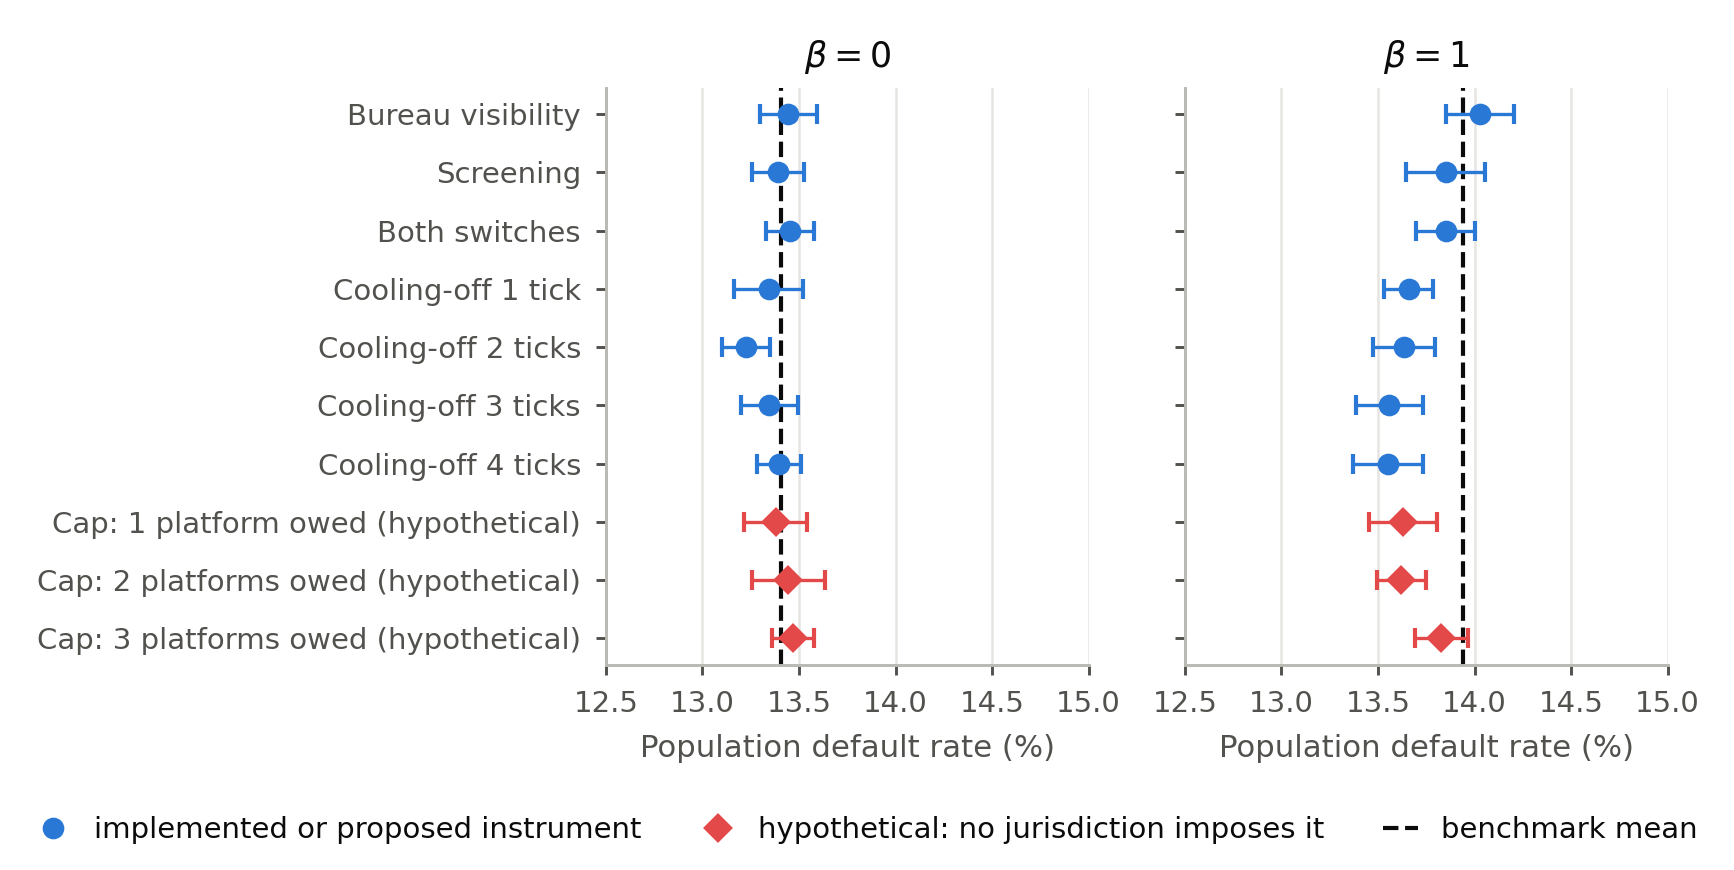
\includegraphics[width=\textwidth]{figures/fig_scenarios_appendix.png}
\caption{Every lever against the benchmark, with and without peer influence}
\label{fig:scenarios-appendix}
\tabnote{The population default rate at the final tick under every implemented lever, at $\beta = 0$ (left) and $\beta = 1$ (right): the two switches of Section~\ref{sec:scenarios} and their combination, the cooling-off window of one to four ticks and the cap of one to three platforms owed. Points are means over 20 replicates with 95\% confidence intervals of the mean; the dashed line is the benchmark mean at the same $\beta$. The cap is hypothetical: no jurisdiction imposes one. Values and differences with standard errors are in Tables~\ref{tab:switches}, \ref{tab:cooloff} and~\ref{tab:cap}.}
\end{figure}

\subsection{Supplementary Sensitivity Results}
\label{app:sensitivity}

Table~\ref{tab:sobol} gives the Sobol decomposition that Section~\ref{sec:results-robustness}
summarises in one sentence; Table~\ref{tab:robustness-appendix} the remaining sensitivity arms, including the
activation-order and population-size checks and the single-tick shock; and
Table~\ref{tab:stacking-full} the platform-count grid at every value of $\beta$. The by-quintile
debt-to-income and zero-savings comparisons (Patterns~3 and~4) are in Tables~\ref{tab:distribution}
and~\ref{tab:bnpl-on-checks}.

% GENERATED by notebooks/scripts/build_results_tables.py from results/raw --
% do not edit by hand; re-run the script instead.
\begin{table}[H]
\centering
\caption{Sobol indices for the population default rate and \ac{BNPL} holding}
\label{tab:sobol}
\tabnote{First-order ($S_1$) and total-order ($S_T$) Sobol indices with 95\% bootstrap confidence half-widths, from a Saltelli design of $N = 256$ base samples over six parameters (2{,}048 design points, 2 replicates each; 4{,}096 runs), \ac{BNPL} on at $\beta$ drawn from its range and every other parameter at its calibrated value. The indices decompose the variance of the final-tick outcome across the ranges shown; an index above one or below zero reflects bootstrap noise. They describe what moves the \emph{level} of default when parameters are uncertain; the \ac{BNPL} \emph{effect}, a difference between arms at fixed parameters, is a separate quantity and is not decomposed here.}
\begingroup\setlength{\tabcolsep}{4pt}\footnotesize
\begin{tabular}{L{4.0cm}c rr rr}
\toprule
& & \multicolumn{2}{c}{Default rate} & \multicolumn{2}{c}{Holding} \\ \cmidrule(lr){3-4}\cmidrule(lr){5-6}
\textbf{Parameter} & \textbf{Range} & \textbf{$S_1$} & \textbf{$S_T$} & \textbf{$S_1$} & \textbf{$S_T$} \\
\midrule
$q_{\text{base}}$ (Submodel 11) & 0.01--0.3 & $0.01 \pm 0.01$ & $0.01 \pm 0.00$ & $0.03 \pm 0.04$ & $0.19 \pm 0.07$ \\
$\beta$ (Submodel 11) & 0--3 & $0.01 \pm 0.02$ & $0.01 \pm 0.00$ & $0.86 \pm 0.28$ & $0.96 \pm 0.22$ \\
minimum-payment fraction (Submodel 6) & 0.025--0.1 & $0.01 \pm 0.01$ & $0.01 \pm 0.00$ & $0.00 \pm 0.01$ & $0.00 \pm 0.00$ \\
$\kappa$ (Submodel 4) & 0.07--0.28 & $0.01 \pm 0.02$ & $0.01 \pm 0.00$ & $0.00 \pm 0.01$ & $0.00 \pm 0.00$ \\
$\lambda$ (Submodel 12) & 0.1--1 & $0.00 \pm 0.01$ & $0.01 \pm 0.00$ & $0.00 \pm 0.01$ & $0.00 \pm 0.00$ \\
shock probability (Submodel 1, fitted) & 0.005--0.026 & $0.99 \pm 0.15$ & $1.00 \pm 0.13$ & $0.01 \pm 0.02$ & $0.01 \pm 0.00$ \\
\bottomrule
\end{tabular}
\endgroup
\end{table}


% GENERATED by notebooks/scripts/build_results_tables.py from results/raw --
% do not edit by hand; re-run the script instead.
\begin{table}[H]
\centering
\caption{Sensitivity of the default rate: remaining arms}
\label{tab:robustness-appendix}
\tabnote{Population default rate at $\beta = 1$, four platforms and full access, for the remaining sensitivity arms, laid out as Table~\ref{tab:robustness}: each group's reference is its default value on the group's own seed set (activation 53{,}000--, population 55{,}000--, minimum-payer share 51{,}000--, minimum payment 52{,}000--, limit 56{,}000--, single-tick shock 58{,}000--, compared with the exact-shortfall reference on 50{,}000--). Means over 20 replicates, replicate standard deviation in brackets; differences are arm less reference, paired by seed with one standard error, except $\ddagger$, where the two arms use different seed blocks or population sizes and the standard error is unpaired. The single-tick shock arm recovers the original one-tick income-loss rule, which no shock probability in range could calibrate to the \ac{CCMR} 90+ band.}
\begingroup\setlength{\tabcolsep}{4pt}\footnotesize
\begin{tabular}{L{7.2cm}rr}
\toprule
\textbf{Arm} & \textbf{Default (\%)} & \textbf{Difference (pp)} \\
\midrule
\multicolumn{3}{l}{\emph{Activation order (Submodel 17)}} \\
random, reseeded each tick & 13.94 (0.34) & reference \\
fixed order, the same every tick & 13.95 (0.30) & $+0.01 \pm 0.10$ \\
\multicolumn{3}{l}{\emph{Population size}} \\
5{,}000 households & 13.85 (0.41) & reference \\
1{,}000 households & 14.21 (0.90) & $+0.35 \pm 0.22^\ddagger$ \\
10{,}000 households & 13.91 (0.42) & $+0.05 \pm 0.13^\ddagger$ \\
\multicolumn{3}{l}{\emph{Minimum-payer share (Submodel 6)}} \\
0.29 (transferred United States estimate) & 14.01 (0.36) & reference \\
0.20 & 13.95 (0.42) & $-0.06 \pm 0.12$ \\
0.25 & 13.98 (0.24) & $-0.03 \pm 0.10$ \\
0.35 & 13.99 (0.41) & $-0.03 \pm 0.12$ \\
0.40 & 13.99 (0.36) & $-0.02 \pm 0.10$ \\
\multicolumn{3}{l}{\emph{Minimum-payment fraction of balance per month (Submodel 6)}} \\
0.05 & 13.89 (0.35) & reference \\
0.025 & 13.79 (0.25) & $-0.10 \pm 0.09$ \\
0.1 & 14.04 (0.38) & $+0.16 \pm 0.11$ \\
\multicolumn{3}{l}{\emph{Rolling per-platform limit $\lambda$, months of income (Submodel 12)}} \\
0.10 & 13.78 (0.29) & reference \\
0.25 & 13.93 (0.33) & $+0.14 \pm 0.10$ \\
0.50 & 13.88 (0.36) & $+0.10 \pm 0.09$ \\
1.00 & 13.88 (0.36) & $+0.10 \pm 0.09$ \\
\multicolumn{3}{l}{\emph{Income-shock persistence (Submodel 1)}} \\
persistent until re-employment (default rule, seeds 50{,}000--) & 14.05 (0.47) & reference \\
single-tick shock & 4.81 (0.04) & $-9.23 \pm 0.11^\ddagger$ \\
\bottomrule
\end{tabular}
\endgroup
\end{table}


% GENERATED by notebooks/scripts/build_results_tables.py from results/raw --
% do not edit by hand; re-run the script instead.
\begin{table}[H]
\centering
\caption{Platform count by peer-influence strength: the full grid}
\label{tab:stacking-full}
\tabnote{Every cell of the stacking experiment: the share of all households holding balances on two or more platforms at the final tick and the population default rate, both replicate means over 20 replicates in per cent (standard deviations at most 0.9 points for the shares and 0.46 for default), for $N$ = one to six platforms and every value of $\beta$ swept. Every run uses the fitted shock probability 0.016 and payment friction 0.09 and access at the banked ceiling; seeds 20{,}000--20{,}019 in every cell. Default at six platforms less default at one: $+0.02 \pm 0.09$pp at $\beta = 0$, $-0.09 \pm 0.07$pp at $\beta = 0.5$, $+0.01 \pm 0.08$pp at $\beta = 1$, $-0.04 \pm 0.12$pp at $\beta = 2$, $+0.14 \pm 0.13$pp at $\beta = 3$, paired by seed with one standard error. Table~\ref{tab:stacking} in the body reports the $\beta = 0$ and $\beta = 1$ columns with dispersion, the holder and over-the-horizon denominators, and cumulative volume.}
\begingroup\setlength{\tabcolsep}{3pt}\footnotesize
\begin{tabular}{c rrrrr rrrrr}
\toprule
& \multicolumn{5}{c}{2+ platforms (\% of households)} & \multicolumn{5}{c}{Default rate (\%)} \\ \cmidrule(lr){2-6}\cmidrule(lr){7-11}
\textbf{$N$} & $\beta=0$ & $\beta=0.5$ & $\beta=1$ & $\beta=2$ & $\beta=3$ & $\beta=0$ & $\beta=0.5$ & $\beta=1$ & $\beta=2$ & $\beta=3$ \\
\midrule
1 & 0.0 & 0.0 & 0.0 & 0.0 & 0.0 & 13.33 & 13.60 & 13.86 & 14.02 & 13.94 \\
2 & 8.5 & 19.7 & 46.8 & 52.9 & 52.9 & 13.51 & 13.47 & 13.92 & 13.90 & 14.04 \\
3 & 9.1 & 23.1 & 54.3 & 60.2 & 60.1 & 13.37 & 13.43 & 13.78 & 13.93 & 14.03 \\
4 & 9.2 & 24.4 & 56.7 & 62.7 & 62.7 & 13.46 & 13.47 & 13.85 & 14.07 & 13.93 \\
5 & 9.3 & 25.3 & 58.5 & 63.9 & 63.7 & 13.44 & 13.52 & 13.85 & 13.99 & 14.10 \\
6 & 9.4 & 25.7 & 59.2 & 64.6 & 64.5 & 13.35 & 13.51 & 13.88 & 13.97 & 14.08 \\
\bottomrule
\end{tabular}
\endgroup
\end{table}


\subsection{Further Extensions}
\label{app:extensions}

Two extensions were considered and are recorded here rather than in
Section~\ref{sec:future-work}, being further from the thesis's own results.

\textbf{Macroeconomic dynamics.} Submodel~16 holds the environment static to protect the
experimental control. A successor design could relax this, since \ac{BNPL} grew in South Africa
through a period of rising rates, and the interaction between \ac{BNPL} stress and a downturn is
what a regulator would want to know. The injection effect and the macro effect would then have to
be separately identified, which requires a more elaborate design than a single counterfactual
injection.

\textbf{Competition among traditional lenders.} The traditional side is a single non-adaptive stub.
Hamill et al. \cite{hamill2023creditcard} show that promotional strategies chosen by
profit-maximising lenders raise borrower indebtedness, so a competing, adapting traditional sector
would add a driver of distress that this model holds fixed.

\section{Variable Construction}
\label{app:variables}

This appendix specifies how every constructed household variable is built, so that each can be
reproduced from the raw survey files without reference to the code. Table~\ref{tab:var-map}
gives the source field, rule and missing-data treatment for every agent field; the subsections
that follow give, for each constructed variable, its source fields, formula, missing-data
treatment, transformations and diagnostics. All monetary values are in 2017 Rands (Part~D.12). The construction follows
Algorithm~\ref{alg:init}, and the last column of Table~\ref{tab:var-map} names the stage
implementing each rule: P1 backbone (\texttt{notebooks/p0\_backbone.ipynb}), P2 match and debt
service (\texttt{p2\_finscope\_match.ipynb}), P3 resample (\texttt{p3\_resample.ipynb}) and P5
instantiation (\texttt{simulation/population.py}).

\begingroup
\setlength{\tabcolsep}{3pt}
\small
\begin{longtable}{L{3.0cm}L{3.2cm}L{3.8cm}L{2.0cm}L{1.3cm}}
\caption{Source field, rule and missing-data treatment for every agent field}
\label{tab:var-map} \\
\multicolumn{5}{p{13.3cm}}{\footnotesize Every agent field of
Table~\ref{tab:agent-mapping}, with the data-layer fields behind them, the survey field or fields it is built from, the rule, what
happens when the source is missing, and the notebook or module implementing the rule. \ac{NIDS}
fields are from the Wave 5 household-derived file unless marked; \ac{FinScope} fields are from the
2019 household file. ``Zero-filled'' means a missing value denotes non-holding and is set to zero,
an assumption tested in Section~\ref{sec:data-validation}. Flows are monthly at this stage and are
scaled to the 14-day tick at instantiation (Part~D.11).} \\
\toprule
\textbf{Agent field} & \textbf{Source field(s)} & \textbf{Rule} & \textbf{If missing} & \textbf{Where} \\
\midrule
\endfirsthead
\toprule
\textbf{Agent field} & \textbf{Source field(s)} & \textbf{Rule} & \textbf{If missing} & \textbf{Where} \\
\midrule
\endhead
\bottomrule
\endfoot
\texttt{income\_monthly} & \texttt{w5\_hhincome} & taken as \ac{NIDS} derives it & record dropped & P1 \\
\addlinespace
\texttt{income\_source} & \texttt{w5\_hhwage}, \texttt{w5\_hhgovt}, \texttt{w5\_hhremitt}, \texttt{w5\_hhother}, \texttt{w5\_hhagric}, \texttt{w5\_hhinvest}, \texttt{w5\_hhcapital} & largest of wage, grant, and the sum of the other five; OTHER if none is positive & zero-filled & P1 \\
\addlinespace
\texttt{income\_wage\_tick} & \texttt{w5\_hhwage} & clipped to $[0, \texttt{w5\_hhincome}]$; $\times\,12/26$ & zero-filled & P5 \\
\addlinespace
\texttt{n\_earners} & \texttt{w5\_empl\_stat} (individual file) & count of roster members recorded as employed & 0 & P5 \\
\addlinespace
\texttt{committed\_tick} & \texttt{w5\_expf} $+$ \texttt{w5\_rentexpend} & food plus rent paid; $\times\,12/26$ & rent zero-filled (80.2\%) & P1, P5 \\
\addlinespace
\texttt{discretionary\_\allowbreak tick} & \texttt{w5\_expnf} & non-food cash expenditure, floored at 0; $\times\,12/26$. Rent is a separate \ac{NIDS} component and is not subtracted; imputed rent (\texttt{w5\_hhimprent}) is excluded & zero-filled & P1, P5 \\
\addlinespace
\texttt{liquid\_savings} & \texttt{w5\_f\_ass} & financial assets, clipped at the 99th percentile (ZAR 133{,}662) & zero-filled (48.2\%) & P1 \\
\addlinespace
\texttt{d\_trad} & \texttt{w5\_f\_deb} & financial debt, as reported & zero-filled (56.6\%) & P1 \\
\addlinespace
\texttt{income\_quintile} & \texttt{w5\_hhincome}, \texttt{w5\_hhsizer}, \texttt{w5\_wgt} & weighted quintiles of income per household member & record dropped & P1 \\
\addlinespace
\texttt{province}, \texttt{household\_size} & \texttt{w5\_prov2011}, \texttt{w5\_hhsizer} & as reported & record dropped & P1 \\
\addlinespace
head demographics & roster \texttt{w5\_r\_relhead}; individual \texttt{w5\_best\_age\_yrs}, \texttt{\_gen}, \texttt{\_race}, \texttt{\_edu} & the roster member coded as head, merged on person identifier & 105 unmatched, retained & P1 \\
\addlinespace
\texttt{banked}; product flags & \ac{FinScope} \texttt{F1}; \texttt{G10}--\texttt{G14} & ``Yes'' $\to$ true; copied as one vector from the matched donor (Appendix~\ref{app:matching}) & ``Don't know'' $\to$ false (14 donors) & P2 \\
\addlinespace
\texttt{apr\_annual}, \texttt{term\_months} & product flags $\times$ rate table & unweighted mean over the classes held; unsecured terms if none & -- & P5 \\
\addlinespace
\texttt{nca\_capacity\_monthly} & \texttt{w5\_hhincome} & $\rho(Y)$: income less the Regulation 23A necessary-expense norm (Table~\ref{tab:reg23a-norms}) & -- & P2, P5 \\
\addlinespace
\texttt{scheduled\_\allowbreak service\_\allowbreak tick} & \texttt{d\_trad}, \texttt{apr\_annual}, \texttt{term\_months}, \texttt{nca\_capacity\_\allowbreak monthly} & $\min\{\mathrm{PMT}(D, \iota, \tau),$ $\rho(Y)\}$; $\times\,12/26$ & 0 if no debt & P2, P5 \\
\end{longtable}
\endgroup

\subsection*{D.1 Sample and weights}

The Wave 5 household-derived file holds 13{,}719 records. A record is retained if
\texttt{w5\_hhincome}, \texttt{w5\_hhsizer} and \texttt{w5\_wgt} are all present and the weight is
positive, leaving 10{,}841. All 2{,}878 dropped records carry a zero or missing weight, so their
removal changes no weighted total; the retained sample represents 18.67 million households.
\texttt{w5\_wgt} is the post-stratified household weight and is used for every weighted statistic
in Section~\ref{sec:population} and as the resampling probability in
Part~D.10; it is not carried onto the agent.

\subsection*{D.2 Monthly income and its source}

\texttt{income\_monthly} is \texttt{w5\_hhincome}, the household income aggregate as \ac{NIDS}
derives it from its component questions; it is not recomposed. \texttt{income\_source} classifies
the household by its largest component: wage (\texttt{w5\_hhwage}), government grant
(\texttt{w5\_hhgovt}), or other, the sum of remittances, other income, agricultural income,
investment income and capital income. Components are zero-filled before comparison, and a
household with no positive component is classed as other. The class gates the employment shock of
Submodel~1: only wage-dominant households are shocked, because grants are statutory transfers.

\texttt{income\_wage\_tick} is the wage component itself, joined at instantiation from
\texttt{w5\_hhwage} on the household identifier, zero-filled where absent and clipped to lie
between zero and total income. It is the base the shock removes: a separation costs the household
one earner's share, \texttt{w5\_hhwage} divided by \texttt{n\_earners}. Every wage-dominant
household has a positive wage component, by the classification rule, and at least one employed
member on the roster, which is asserted at load; both hold for all 3{,}038 wage-dominant agents
(1{,}841 distinct source households).

\subsection*{D.3 Employed members}

\texttt{n\_earners} is the count of roster members whose \texttt{w5\_empl\_stat} in the individual
file is ``Employed'', merged on the household identifier; households with no such member take
zero. It makes the separation probability a per-earner hazard, directly comparable to the
individual transition rate in the \ac{QLFS}, and it is why losing one earner in a two-earner
household costs half the wage component rather than all of it.

\subsection*{D.4 Committed and discretionary expenditure}

\ac{NIDS} total expenditure decomposes exactly into four disjoint components, food
(\texttt{w5\_expf}), non-food (\texttt{w5\_expnf}), rent paid (\texttt{w5\_rentexpend}) and
imputed rent (\texttt{w5\_hhimprent}), and the decomposition is asserted at construction to
within five cents. \texttt{committed\_tick} is food plus rent paid, the incompressible floor;
\texttt{discretionary\_tick} is non-food, floored at zero. Rent is not subtracted from non-food,
because \ac{NIDS} records it as a separate component that non-food already excludes. Imputed
rent, the consumption value of owner-occupied housing, is a non-cash item and is excluded from
both tiers; including it would have inflated compressible consumption by a median of ZAR 700 per
month for the 82.6\% of households assigned an imputed rent. Rent paid is zero-filled for the
80.2\% of households that report none, so for them committed expenditure is food alone.

The non-food aggregate already contains reported clothing-account and hire-purchase payments
(median 12.6\% of non-food outlay among the 11.2\% of sample households reporting one) and
vehicle-finance payments, so the constructed servicing of Part~D.9 charges a flow partly present
in discretionary spending (Section~\ref{sec:servicing}). This overstates compressible outlay for
indebted agents and understates their servicing share of outlay; its net effect on distress and
on scenario differences is unsigned. The label ``discretionary''
also covers transport, utilities and education, none of which is discretionary in the ordinary sense,
because \ac{NIDS} offers no finer split.

\subsection*{D.5 Liquid savings}

\texttt{liquid\_savings} proxies an accessible cash buffer by \texttt{w5\_f\_ass}, reported
financial assets. The field follows a gateway question and records a value only where the
household reports holding financial assets, so a missing value denotes non-holding and is set to
zero (48.2\% of households); the field never records a literal zero, which is asserted before the
fill. The distribution is clipped at its unweighted 99th percentile over all households, zeros
included, ZAR 133{,}662, to limit the influence of
a small number of extreme reports. This is the weakest field in the layer, since reported
financial assets are neither necessarily liquid nor necessarily accessible, and validation
pattern~4 (the share of agents reaching zero savings) is judged against it.

\subsection*{D.6 Traditional debt}

\texttt{d\_trad} is \texttt{w5\_f\_deb}, reported financial debt, zero-filled for the 56.6\% of
households recording none on the same gateway logic as savings. The aggregate is the external
test of the zero-fill: total synthetic debt is 49\% of the \ac{CCMR} gross debtor book for the
in-scope products; imputing the missing entries at holder means would give 111\% of the same
book, more than the bureau records.
\ac{NIDS} reports one consolidated balance, so nothing in the construction can weight rates or
terms by product.

\subsection*{D.7 Income quintile}

\texttt{income\_quintile} is assigned on income per household member,
\texttt{w5\_hhincome}/\texttt{w5\_hhsizer}, using cut points that put one fifth of weighted
households in each class (a household at a cut point falls in the lower class): ZAR 900, 1{,}801, 3{,}400 and 7{,}712 per person per month. The
quintile is both a reporting category and, crossed with province, the matching cell of
Appendix~\ref{app:matching} and the reference group of Submodel~11. \ac{FinScope} donors are
assigned to the same cut points from the midpoint of a seven-band income question divided by
household size.

\subsection*{D.8 Financial-inclusion flags}

\texttt{banked} is \ac{FinScope} \texttt{F1} equal to ``Yes''; the five product flags are
\texttt{G10} to \texttt{G14} (store card, revolving credit, hire purchase, short-term loan,
personal loan) equal to ``Yes''. All six are copied as one vector from a single donor drawn within
the household's quintile-by-province cell in proportion to the donor's weight; the procedure,
its assumptions and its limits are Appendix~\ref{app:matching}. Lay-by (\texttt{G15}) is excluded
as not credit. The flags are categorical and are not deflated.

\subsection*{D.9 Debt service}
\label{app:var-servicing}

\texttt{scheduled\_service\_tick} converts the debt stock to a monthly flow in three steps.

\emph{Rate and horizon.} Each product class carries the \ac{NCA} statutory maximum rate at the
2017 repurchase rate of 7.00\% and a repayment horizon (Table~\ref{tab:credit-terms}). A
household's rate and horizon are the unweighted means over the classes its donor flags; the
74.0\% of donors flagging none are priced as unsecured (28\%, 25 months). Store-card and
hire-purchase horizons are measured in \ac{NIDS} as the median ratio of the household's total
financial debt to its observed monthly payment for that product, among households paying only
that product ($n = 782$ and $121$); because
the numerator is the whole balance and the denominator a single product's payment, these are
upper bounds on the true horizon. Personal-loan and unflagged horizons are the \ac{CCMR}
stock-flow implied life of the unsecured book, three times the gross debtors book divided by
quarterly credit granted (24.8 months); the short-term horizon is one month by product
definition; revolving credit, which has no contractual term, takes the reciprocal of the
default minimum-payment fraction, 0.05 (20 months). A one-month floor on the term is a numerical
guard only and never binds.

\emph{Amortisation.} The uncapped instalment is the level monthly payment,
$\mathrm{PMT}(D, \iota, \tau) = D\,r / (1 - (1+r)^{-\tau})$ with $r = \iota/12$.

\emph{Affordability cap.} The instalment is capped at $\rho(Y)$, the monthly debt service the
Regulation 23A residual-income test permits: gross monthly income less the statutory minimum
necessary expenses for the household's income band (Table~\ref{tab:reg23a-norms}). The cap binds
for 3.8\% of indebted households ($n = 178$) and removes 22.8\% of aggregate calculated service.
Fifty-three indebted households (27 agents after resampling) have income at or below ZAR 800,
the first band boundary, where the norm equals
income and capacity is zero; they enter the model holding debt with no scheduled service, since
the data cannot say whether the debt is legacy, informal or non-compliant. The same function is
the credit-granting gate of Submodel~9, so the data layer and the model apply one test. Across the 4{,}702
indebted source households the resulting debt-service-to-income ratio has a weighted mean of
10.9\% and an unweighted median of 3.3\%; the weighted full-population mean is 4.8\%, since
56.0\% of weighted households hold no debt.

\begin{table}[H]
\centering
\caption{Regulation 23A minimum necessary-expense norms}
\label{tab:reg23a-norms}
\tabnote{The statutory table of minimum monthly necessary expenses by gross monthly income band,
from the Affordability Assessment Regulations \cite{sa_ncr_affordability_2015}. For income $Y$ in
a band, necessary expenses are the fixed amount plus the percentage of income above the band's
lower bound; residual-income capacity is $\rho(Y) = Y$ less that amount. The implementation is
asserted against the regulation's two published worked examples (ZAR 2{,}000 $\to$ 881.00; ZAR
10{,}000 $\to$ 1{,}505.38). The regulation is written for an individual consumer and is applied
here to household income, which makes the test more permissive for multi-earner households
(Appendix~\ref{app:gate}); across the population the resulting ceiling spans 0 to 93.2\% of gross
income, with a mean of 49.6\% in the bottom quintile.}
\begin{tabular}{rrr}
\toprule
\textbf{Lower bound (ZAR)} & \textbf{Fixed (ZAR)} & \textbf{Plus \% above bound} \\
\midrule
0.00 & 0.00 & 100.00 \\
800.01 & 800.00 & 6.75 \\
6{,}250.01 & 1{,}167.88 & 9.00 \\
25{,}000.01 & 2{,}855.38 & 8.20 \\
50{,}000.01 & 4{,}905.38 & 6.75 \\
\bottomrule
\end{tabular}
\end{table}

\emph{Diagnostics.} Among indebted households, constructed servicing is 12.8\% of monthly
outlay, against a \ac{FinScope} self-reported range of 6.1--9.8\% among holders of a modelled
product. The excess is in the direction ceiling rates imply, and the double count of Part~D.4
inflates the outlay denominator, so removing it would widen the gap.

\subsection*{D.10 Resampling}
\label{app:var-resample}

The 10{,}841 weighted households are resampled with replacement, with probability proportional
to \texttt{w5\_wgt} (seed 20260818), to 5{,}000 unweighted agents drawn from 3{,}221 unique
source records. Every downstream statistic is therefore unweighted. The resample raises the
per-capita income Gini from 0.6514 to 0.6668; its fidelity on the categorical attributes is
within 1.4 percentage points (Figure~\ref{fig:pop-fidelity}).

\subsection*{D.11 Tick scaling}
\label{app:var-tick}

Survey flows are monthly and the model's tick is 14 days, so every flow is multiplied once, at
instantiation, by $\chi = 12/26$: income, its wage component, committed and discretionary
expenditure, and scheduled service. Three monthly quantities are kept unscaled because the rules
that use them are specified monthly: \texttt{income\_monthly} and \texttt{nca\_capacity\_monthly}
for the Regulation 23A test, and \texttt{discretionary\_monthly} for sizing \ac{BNPL} purchases,
which are lumpy monthly-scale items rather than fortnightly flows. Stocks (savings and debt) are
not scaled. Per-tick interest is the annual rate divided by 26, matching the monthly convention
of the amortisation rather than compounding it.

\subsection*{D.12 Deflation}
\label{app:var-deflation}

Nothing in the \ac{NIDS} or \ac{FinScope} layer is deflated: monetary values are 2017 Rands as
surveyed, and the imputed flags are categorical. The only deflated quantities are three
\ac{BNPL} parameters at 2026 prices, the assumed per-order cap (ZAR 15{,}000
$\to$ 9{,}927) and Payflex's published late fee (ZAR 95 a week, ZAR 190 per tick $\to$ 125.74) and fee cap
(ZAR 285 $\to$ 188.61), which are converted once by a cumulative price factor taken from published Stats SA \ac{CPI}
releases \cite{statssa_cpi}; the factor reproduces the published index to within 0.8\%. The
purchase-size ratio $\kappa$ is a share of the household's own discretionary budget and needs no
deflation.

\section{Cell-Donor Matching: Procedure, Assumptions and Limits}
\label{app:matching}

Figure~\ref{fig:cell-donor} illustrates the procedure, Algorithm~\ref{alg:match} specifies the
steps, and Table~\ref{tab:notation} defines the notation.

\subsection*{E.1 The procedure}

Both surveys are partitioned by the same two variables, per-capita income quintile $q$ and
province $p$, into $|\mathcal{C}| = 45$ cells $c = (q, p)$. For each \ac{NIDS} record $i$ with
cell $c(i)$, one donor $d$ is drawn from the \ac{FinScope} records in the same cell with
probability $w_d / \sum_{d' \in c(i)} w_{d'}$, where $w$ is the \ac{FinScope} household weight,
and the donor's six-flag vector (banked; store card; revolving credit; hire purchase; short-term
loan; personal loan) is copied to $i$ in its entirety. Draws are with replacement, seeded (42), and
the quintile of a \ac{FinScope} donor is assigned from the midpoint of its seven-band income
question divided by household size, against the weighted \ac{NIDS} quintile bounds. The
procedure is specified to fall back to the quintile-only pool if a cell is empty; no draw ever did.

The smallest cell holds 30 donors and the median 87; only three cells (all in the top
quintile: Limpopo, North West, Northern Cape) hold fewer than 50. Of 4{,}969 available donors,
3{,}597 were used at least once; the median donor was used twice, the 99th percentile 13 times,
and the most-used donor 20 times. Donor reuse is concentrated where \ac{NIDS} is dense and
\ac{FinScope} is thin: in the largest cell, the bottom quintile of KwaZulu-Natal, 1{,}058
recipients drew from 109 donors, and eleven cells have more than three recipients per donor.
The heaviest 1\% of donors nonetheless supply only 5.1\% of recipients.

\subsection*{E.2 Assumptions under which the match is credible}

\begin{description}
\item[A1. Cell sufficiency.] Conditional on income quintile and province, the six flags are
independent of everything else in \ac{NIDS} that affects a household's behaviour in the model.
This assumption cannot be tested from the two surveys alone, since the flags
are observed in one and the balance sheet in the other. Its defence is that quintile and
province are the two strongest correlates of financial inclusion available in \emph{both}
instruments, and that the \ac{FinScope} flags show large between-cell variation along both
(banked status ranges from below 60\% to above 95\% across cells).
\item[A2. Common support.] Every \ac{NIDS} cell has \ac{FinScope} donors. Verified, not
assumed: at least 30 in each of 45 cells, and zero fallback draws.
\item[A3. Population comparability.] The two instruments sample the same population, and a
donor's answers stand for its household. \ac{FinScope} interviews one adult per household, chosen
by Kish grid, and asks about accounts and credit in that adult's own name (\texttt{F1},
\texttt{G10}) or used in the past twelve months (\texttt{G11}--\texttt{G14}). The imputed flags
therefore record one adult's holdings and understate holding in households with several adults.
The product questions name the same instruments the \ac{CCMR} categorises, which is what lets
each flag be priced from the statutory rate table.
\item[A4. Joint-structure preservation.] Because one donor supplies all six flags, the imputed
joint distribution of products within a cell follows the weighted donor distribution in
expectation. Finite draws need not reproduce it exactly. This is why single-donor transfer was chosen over per-flag imputation
(Figure~\ref{fig:cell-donor}c), and it matters because the combination of products a
household holds prices its opening traditional debt.
\item[A5. Weight-proportional draw.] Drawing in proportion to \ac{FinScope} weight reproduces
that survey's weighted cell marginals in expectation. Table~\ref{tab:imputation_errors}
(national, 1.8 points at most) and the by-quintile check (2.3 points at most) test it; national
gaps also absorb differences between the two surveys' cell compositions.
\end{description}

\subsection*{E.3 Circumstances under which the match is problematic}

\begin{description}
\item[P1. Within-cell heterogeneity.] Anything that predicts inclusion within a cell, urban or
rural location above all, and also education and the formality of employment, is not matched
on. Donor flags still vary within each cell, but their associations with these recipient
characteristics are lost. If those associations concentrate borrowing among liquidity-constrained
households, the model may understate exposure concentration. The direction and size of that
effect are not established by the marginal checks.
\item[P2. Small-cell donor reuse.] Recipients are drawn with replacement from pools that in
three cells are near the 30-donor floor, and in the densest cells outnumber donors nearly ten
to one. A heavily reused donor's flag vector is stamped onto many recipients, which reduces the
effective sample of flag vectors below the nominal 10{,}841. The 5.1\% concentration figure of
Part~E.1 is national and does not bound concentration within a cell.
\item[P3. Matching-key error.] \ac{FinScope} income is banded and in 2019 Rands, so a donor's
quintile rests on a band midpoint divided by household size and placed against 2017 cut points.
Donors therefore do not split evenly into fifths, and misassignment across a quintile boundary
places a donor in the wrong cell.
\item[P4. Respondent, not household.] Because \ac{FinScope} records one adult's holdings
(A3), a multi-adult household is imputed the inclusion of one member. Banked status, which gates
\ac{BNPL} eligibility, and the product flags that price opening debt are therefore likely to be
understated for larger households; the direction on default is not established.
\item[P5. Vintage.] The flags are 2019 observations imposed on a 2017 population. Banked status
was rising over that interval, so the 82.8\% \ac{BNPL}-eligibility ceiling is plausibly
too generous for 2017. The magnitude is unknown, and the categorical flags cannot be deflated.
\item[P6. Group B validation is a construction check.] Because the draw is weight-proportional
within the cell, agreement with the \ac{FinScope} cell marginals is expected by construction.
The seven Group B checks in Table~\ref{tab:validation} therefore verify the implementation and
say nothing about the population's external validity; Section~\ref{sec:data-validation} counts
them accordingly.
\item[P7. The joint distribution is never externally validated.] Only marginals are checked. No
independent South African benchmark was located for the joint distribution of credit-product
holding. Copying observed combinations supports plausibility but does not verify the resulting
joint distribution in the recipient population.
\end{description}

\subsection*{E.4 Which of these would move a result}

The vintage gap (P5) and the one-adult respondent (P4) can change the eligibility ceiling and
adoption levels, in opposite directions.
The access sweep tests sensitivity to eligibility levels, but does not reconstruct who was banked
in 2017. Lost within-cell associations (P1) can affect both the distribution of exposure and
aggregate default, since household responses are nonlinear.
Donor reuse and income-band error (P2--P3) are not ranked. P6--P7 limit the validation claim: agreement on construction targets cannot establish
that the imputed population reproduces unobserved relationships.

The alternative not taken, a distance-based or model-based fusion on more matching variables recovering finer joint structure
from both instruments, is recorded in Appendix~\ref{app:rationale}. It would relax A1 at the
cost of its own validation burden and the risk of fitting the idiosyncrasies of two surveys
rather than the population behind them; the cell match reproduces cell marginals and keeps each
donor's product combination, the two things the model consumes.

\subsection*{E.5 Fidelity of the match and the resample}

Table~\ref{tab:imputation_errors} and Figure~\ref{fig:inclusion-fidelity} compare the imputed
indicators with their \ac{FinScope} targets, nationally and by quintile.
Figure~\ref{fig:pop-fidelity} compares the 5{,}000-agent resample with its source
(Section~\ref{sec:resample}).

\begin{table}[H]
\centering
\caption{National rates for the six imputed indicators}
\label{tab:imputation_errors}
\tabnote{This table compares the national rate of each imputed indicator in three populations: the \ac{FinScope} 2019 target, weighted by its survey weight; the 10{,}841-household synthetic population after matching, weighted by \ac{NIDS} survey weight; and the unweighted 5{,}000-agent resample used in the simulation. The difference column is synthetic less \ac{FinScope}, in percentage points, computed before rounding; the tolerance is 3 percentage points (Table~\ref{tab:validation}). Because the match draws donors within the same quintile-by-province cell in proportion to weight, agreement here is expected by construction: it tests the implementation, not the population's external validity (Section E.2).}
\begin{tabular}{lrrrr}
\toprule
\textbf{Imputed indicator} & \textbf{FinScope 2019} & \textbf{Synthetic} & \textbf{Agents} & \textbf{Difference} \\
 & \textbf{(\%)} & \textbf{(\%)} & \textbf{(\%)} & \textbf{(pp)} \\
\midrule
Banked status    & 82.4 & 82.8 & 82.8 & 0.4 \\
Store card       & 20.8 & 22.6 & 21.8 & 1.8 \\
Revolving credit &  3.7 &  4.1 &  3.8 & 0.5 \\
Hire purchase    &  6.5 &  6.9 &  6.5 & 0.5 \\
Short-term loan  &  2.7 &  3.4 &  3.3 & 0.6 \\
Personal loan    &  2.1 &  2.3 &  2.3 & 0.2 \\
\bottomrule
\end{tabular}
\end{table}

\begin{figure}[H]
\centering
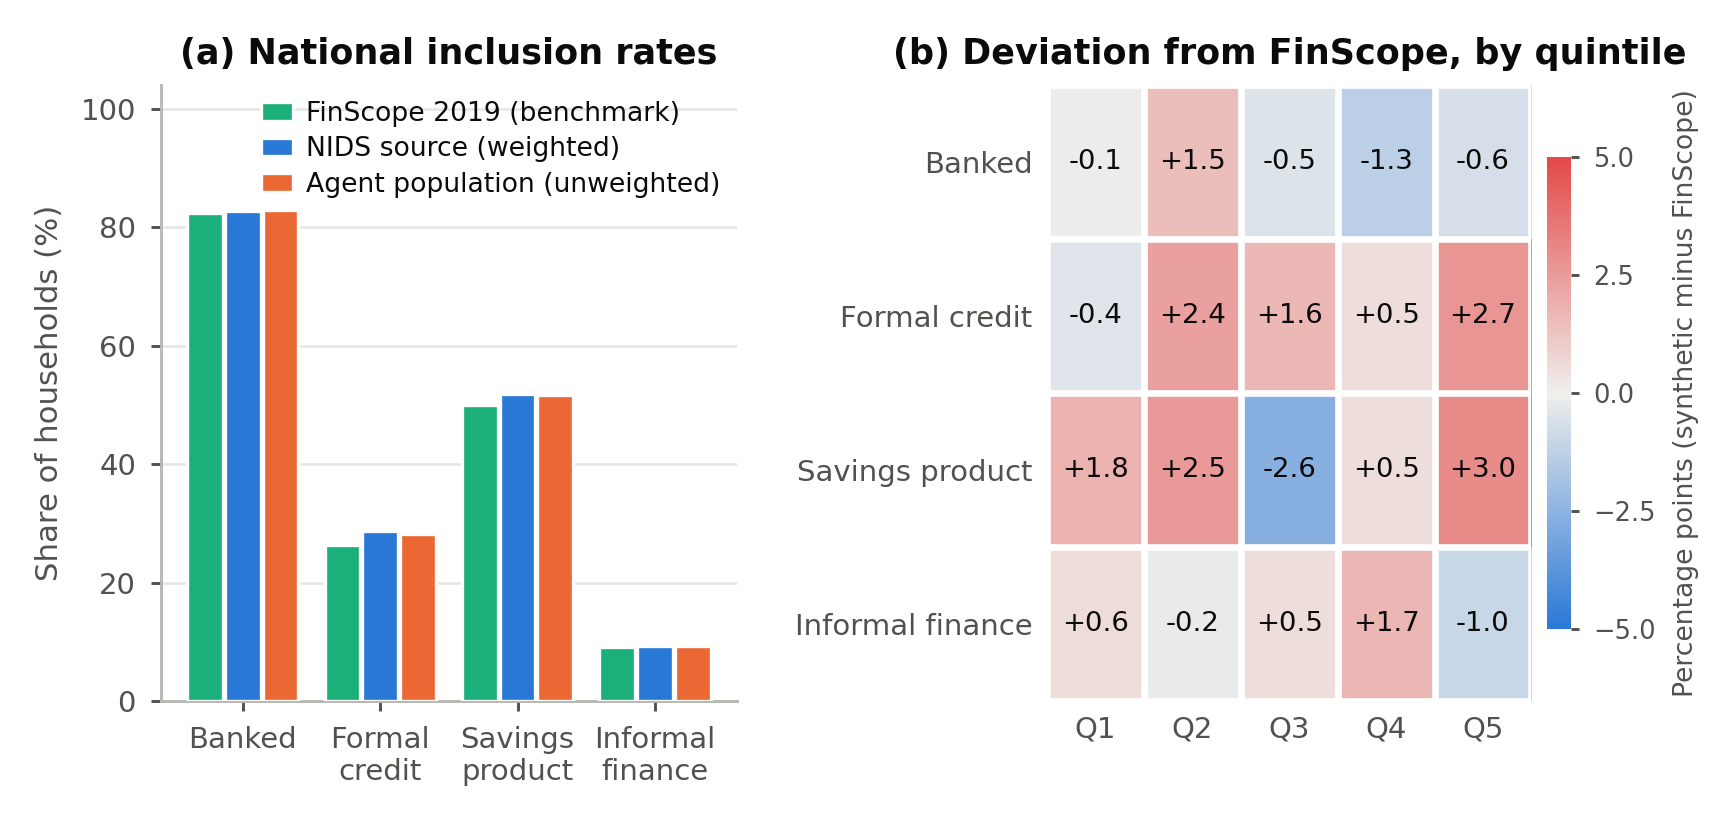
\includegraphics[width=\textwidth]{figures/fig_inclusion_fidelity.png}
\caption{Fidelity of the imputed indicators}
\label{fig:inclusion-fidelity}
\tabnote{Panel (a) compares the national rate of each of the six imputed indicators across the \ac{FinScope} 2019 target, the weighted synthetic population and the unweighted 5{,}000-agent population, as in Table~\ref{tab:imputation_errors}. Panel (b) shows the synthetic-less-\ac{FinScope} gap for each indicator within each per-capita income quintile, thirty cells in all; the largest single deviation is 2.3 percentage points against a tolerance of 5. Quintiles are the weighted \ac{NIDS} bounds of Appendix~\ref{app:variables}.}
\end{figure}

\begin{figure}[H]
\centering
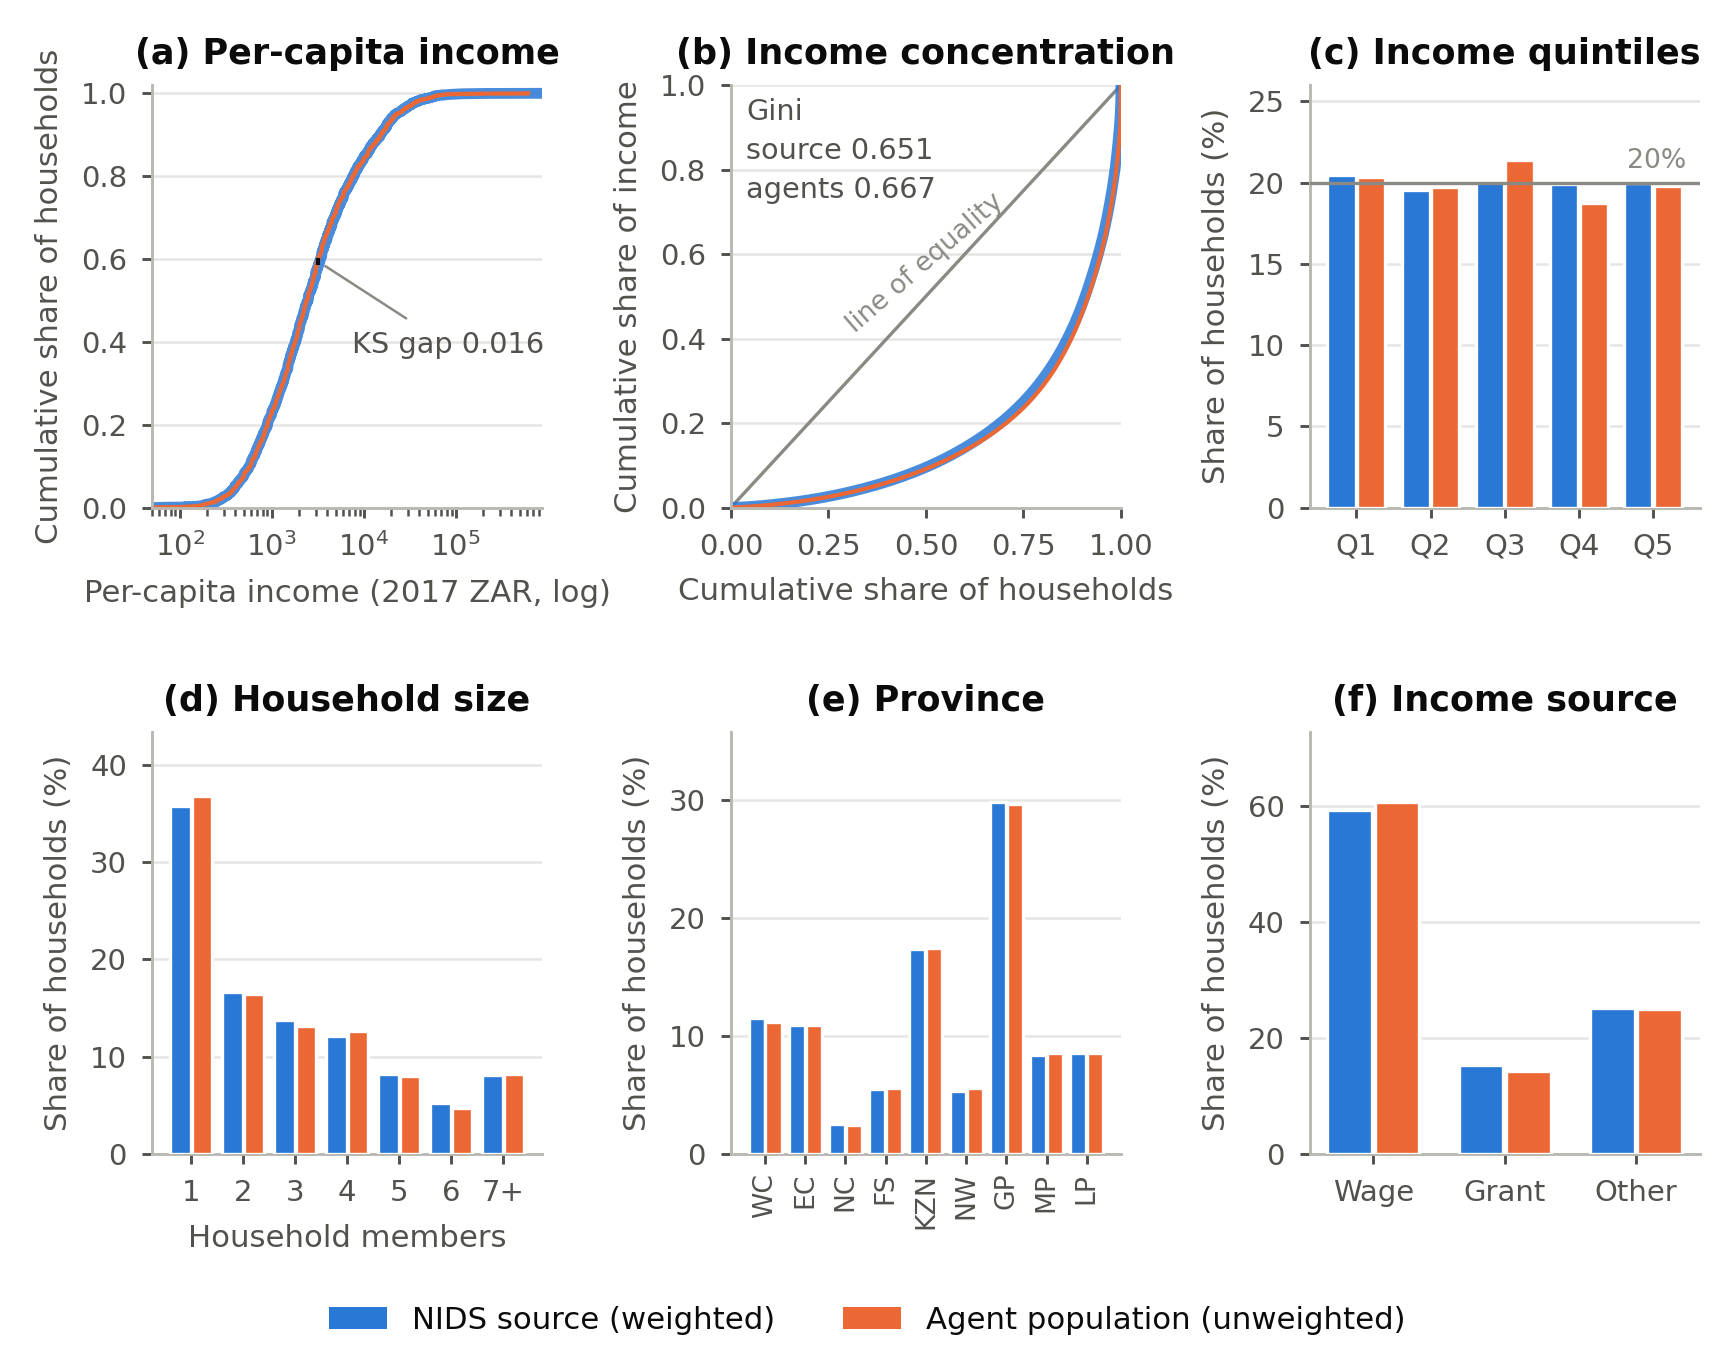
\includegraphics[width=\textwidth]{figures/fig_population_fidelity.png}
\caption{Distributional fidelity of the agent population}
\label{fig:pop-fidelity}
\tabnote{Each panel compares the unweighted 5{,}000-agent resample, drawn with replacement in proportion to \ac{NIDS} survey weight (seed 20260818) from 3{,}221 unique source records, against the weighted 10{,}841-household source it is drawn from. Panels (a) and (b) cover the per-capita income distribution and its concentration; panels (c) to (f) cover income quintile, household size, province and primary income source, the categorical attributes that gate behaviour and define the reference groups in the simulation. The Kolmogorov--Smirnov distance in (a) is 0.016, the largest categorical deviation across the 24 sub-categories is 1.4 percentage points, and the Gini rises by 0.015, from 0.6514 to 0.6668.}
\end{figure}

\section{Pseudocode: Notation and Initialisation}
\label{app:pseudo-init}

This appendix and Appendix~\ref{app:pseudo-main} give the model as pseudocode, following the
convention of a master algorithm that dispatches to sub-algorithms. The algorithms are the
normative statement of the pipeline: where prose elsewhere in the thesis and an algorithm here
differ, the algorithm governs, and each has been checked line by line against the module that
implements it (\texttt{simulation/}). Three robustness arms change a rule without a switch shown
here: the single-tick income shock (Submodel~1), purchases sized on $Y_i$ in place of $E^d_i$
(Submodel~4) and a fixed activation order (Submodel~17). Table~\ref{tab:notation} fixes the notation used throughout.
Sets are in script capitals, $H$ and $P$ are the sizes of $\mathcal{H}$ and $\mathcal{P}$, and
elements are in lower case; a
subscript indexes an element, a superscript identifies a variant. Random draws are written
$U(0,1)$; every draw within a run comes from generators seeded by the run's seed. The threshold
endowments $\theta_i$ come from a separate initialisation stream so that control arms reproduce
the main stream exactly, and the order of activation and the resampling of populations other
than 5{,}000 each use their own generator.

\begingroup
\small
\begin{longtable}{L{2.6cm}L{7.4cm}L{3.4cm}}
\caption{Notation}
\label{tab:notation} \\
\multicolumn{3}{p{13.4cm}}{\footnotesize This table defines every symbol used in
Algorithms~\ref{alg:init} to~\ref{alg:peer}. Flows are per 14-day tick unless marked monthly; all
money is in 2017 Rands. The right-hand column names the parameter in
\texttt{simulation/config.py}, or the field, method or function in \texttt{simulation/}, that
carries the quantity, so that a symbol can be traced to code. Symbols already used in the body
(Equation~\ref{eq:peer}) are unchanged.} \\
\toprule
\textbf{Symbol} & \textbf{Meaning} & \textbf{Code} \\
\midrule
\endfirsthead
\toprule
\textbf{Symbol} & \textbf{Meaning} & \textbf{Code} \\
\midrule
\endhead
\bottomrule
\endfoot
\multicolumn{3}{l}{\emph{Sets and indices}} \\
$\mathcal{H}$, $H$, $i$ & households, their number ($5{,}000$), a household & \texttt{n\_agents} \\
$\mathcal{P}$, $P$, $p$ & \ac{BNPL} platforms, their number (4), a platform & \texttt{n\_platforms} \\
$\mathcal{G}$, $g(i)$ & reference groups (income quintile $\times$ province, 45); the group of $i$ & \texttt{reference\_group} \\
$c(i)$ & the matching cell of $i$ in the data layer; the same partition as $g(i)$ & -- \\
$q(i)$, $p(i)$ & income quintile and province of $i$, in the data layer only; elsewhere $q$ is a purchase propensity and $p$ a platform & \texttt{income\_quintile}, \texttt{province} \\
$t$, $T$, $T_0$ & tick, horizon (52), burn-in (12) & \texttt{n\_ticks}, \texttt{burn\_in} \\
$\chi$ & monthly-to-tick conversion, $12/26$ & \texttt{MONTHLY\_TO\_TICK} \\
\addlinespace
\multicolumn{3}{l}{\emph{Household constants, from the data layer}} \\
$\text{source}_i$ & dominant income source: WAGE, GRANT or OTHER & \texttt{income\_source} \\
$y_i$, $y^w_i$ & income per tick; its wage component & \texttt{income\_tick}, \texttt{income\_wage\_tick} \\
$Y_i$, $E^d_i$ & monthly income; monthly discretionary budget & \texttt{income\_monthly}, \texttt{discretionary\_monthly} \\
$n_i$ & employed members on the roster & \texttt{n\_earners} \\
$e^c_i$, $e^d_i$ & committed expenditure; discretionary target, per tick & \texttt{committed\_tick}, \texttt{discretionary\_tick} \\
$\tau_i$ & term (months) pricing the opening balance & \texttt{term\_months} \\
$\rho_i = \rho(Y_i)$ & Regulation 23A monthly residual-income capacity & \texttt{nca\_capacity\_monthly} \\
$\epsilon_i$, $m_i$ & indicators: \ac{BNPL}-eligible; minimum-payer archetype & \texttt{bnpl\_eligible}, \texttt{is\_min\_payer} \\
$\theta_i$ & adoption threshold (threshold mechanism only) & \texttt{theta} \\
$w_i$ & survey weight (data layer only) & \texttt{w5\_wgt} \\
\addlinespace
\multicolumn{3}{l}{\emph{Household state at tick $t$}} \\
$a_i(t)$ & liquid savings & \texttt{savings} \\
$u_i(t)$ & earners currently unemployed & \texttt{n\_unemployed} \\
$D_i(t)$, $A_i(t)$ & traditional debt; traditional arrears & \texttt{d\_trad}, \texttt{arrears\_trad} \\
$r_i(t)$, $\iota_i(t)$ & scheduled traditional debt service per tick; annual rate on the consolidated balance. Both open at the data-layer values and move when a traditional loan is booked (Algorithm~\ref{alg:gate}); $r_i$ returns to zero when the balance clears & \texttt{scheduled\_service\_tick}, \texttt{apr\_annual} \\
$B_{ip}(t)$ & \ac{BNPL} receivable owed by $i$ to platform $p$ & \texttt{exposure} \\
$b_i(t)$ & \ac{BNPL} instalments and arrears falling due this tick, all platforms; an agreement opened this tick is excluded & \texttt{bnpl\_due\_per\_tick} \\
$o_i(t)$ & one instalment for each live \ac{BNPL} agreement plus arrears, all platforms, including agreements opened this tick; what a gate that sees \ac{BNPL} is shown & \texttt{bnpl\_obligations\_per\_tick} \\
$n^{\text{owed}}_i(t)$ & platforms on which $i$ owes a balance & \texttt{stacking\_depth} \\
$\alpha_i(t)$ & ticks in traditional arrears & \texttt{arrears\_age\_ticks} \\
$\delta_i(t)$ & consecutive distressed ticks & \texttt{distress\_streak} \\
$d_i(t)$ & default indicator & \texttt{defaulted} \\
$\bar t_i$ & tick until which want-driven purchases are blocked & \texttt{cool\_off\_until} \\
$s_g(t)$ & share of the eligible members of $g$ holding a \ac{BNPL} balance at the end of $t$ & \texttt{group\_share\_lagged} \\
\addlinespace
\multicolumn{3}{l}{\emph{Platform constants}} \\
$L_{ip}$ & rolling receivable limit of $p$ for $i$, $L_{ip} = \lambda Y_i$ & \texttt{rolling\_limits} \\
$\bar o$ & per-order cap & \texttt{bnpl\_order\_cap} \\
$N$ & instalments per order (4) & \texttt{bnpl\_instalments} \\
$\phi$, $\bar\phi$ & late fee per missed tick; fee cap per agreement in Rand. The cap applied is the lower of $\bar\phi$ and half the purchase price & \texttt{bnpl\_late\_fee\_*} \\
\addlinespace
\multicolumn{3}{l}{\emph{Parameters}} \\
$p^{\text{sep}}$, $p^{\text{exit}}$ & per-earner separation and re-employment probabilities per tick & \texttt{shock\_prob}, \texttt{shock\_exit\_prob} \\
$\pi$ & payment friction: probability of skipping an affordable traditional instalment & \texttt{payment\_friction} \\
$f^{\min}$ & minimum-payment fraction of balance per month & \texttt{min\_payment\_frac} \\
$k$ & distressed ticks that trigger default (7) & \texttt{k\_default} \\
$\varphi$ & discretionary floor as a share of target (0 by default) & \texttt{discretionary\_floor} \\
$\kappa$, $\nu$ & purchase-size ratio to $E^d_i$; its coefficient of variation & \texttt{bnpl\_purchase\_ratio}, \texttt{\_cv} \\
$\mathbb{1}^{\text{cap}}$ & cap on the \ac{BNPL} share of a shortfall request at $\kappa E^d_i$ (off only in the three uncapped robustness arms) & \texttt{shortfall\_bnpl\_capped} \\
$\mathbb{1}^{\text{short}}$ & \ac{BNPL} may relieve a shortfall (off only in one robustness arm) & \texttt{shortfall\_bnpl} \\
$\mathbb{1}^{\text{fund}}$ & credit raised against a committed shortfall pays it first (on only in one robustness arm) & \texttt{committed\_shortfall\_funded} \\
$\mathbb{1}^{\text{loyal}}$ & platforms already owed are tried first (on only in one robustness arm) & \texttt{platform\_routing} \\
$\lambda$ & rolling limit as a multiple of monthly income & \texttt{bnpl\_limit\_income\_multiple} \\
$q_{\text{base}}$, $\beta$ & base propensity; peer weight (linear mechanism) & \texttt{q\_base}, \texttt{beta} \\
$\gamma$, $\mu_\theta$, $\sigma_\theta$ & appetite step; threshold mean and dispersion (threshold mechanism) & \texttt{gamma}, \texttt{mu\_theta}, \texttt{sigma\_theta} \\
$k^{\text{cool}}$, $\bar n$ & cooling-off ticks; cap on the number of platforms owed (both off in the benchmark) & \texttt{k\_cool}, \texttt{stacking\_cap} \\
\addlinespace
\multicolumn{3}{l}{\emph{Scenario switches}} \\
$\mathbb{1}^{\text{bnpl}}$ & \ac{BNPL} platforms present (off in the calibration baseline) & \texttt{bnpl\_enabled} \\
$\mathbb{1}^{\text{bur}}$ & \ac{BNPL} obligations visible to the bureau (bureau visibility) & \texttt{bnpl\_bureau\_visible} \\
$\mathbb{1}^{\text{aff}}$ & Regulation 23A test applied to \ac{BNPL} originations (screening) & \texttt{bnpl\_affordability\_check} \\
\addlinespace
\multicolumn{3}{l}{\emph{Functions}} \\
$\rho(Y)$ & Regulation 23A residual-income capacity: $Y$ less the statutory necessary-expense norm (Table~\ref{tab:reg23a-norms}) & \texttt{nca\_max\_service} \\
$\mathrm{PMT}(D, \iota, \tau)$ & level monthly instalment amortising $D$ at annual rate $\iota$ over $\tau$ months & \texttt{amortised\_instalment} \\
$\mathrm{clip}(x, 0, 1)$ & $\min(\max(x, 0), 1)$ & -- \\
\end{longtable}
\endgroup

\subsection*{F.1 The master algorithm}

Initialisation has four stages, each a sub-algorithm. The first three and the draw of 5{,}000
records that opens the fourth are the data layer of Section~\ref{sec:population}, run once
offline to produce the population file; the rest of the fourth runs at the start of every
simulation and turns that file into agents. Algorithm~\ref{alg:init} dispatches them.

\begin{algorithm}[H]
\caption{Initialisation}
\label{alg:init}
\begin{algorithmic}
\State Build the survey backbone: execute Algorithm~\ref{alg:backbone}
\State Impute financial-inclusion flags: execute Algorithm~\ref{alg:match}
\State Construct debt service: execute Algorithm~\ref{alg:service}
\State Resample to $H$ agents and instantiate the model: execute Algorithm~\ref{alg:resample}
\end{algorithmic}
\end{algorithm}

\subsection*{F.2 Build the survey backbone}

Algorithm~\ref{alg:backbone} filters the \ac{NIDS} household file and derives the six core
variables of Section~\ref{sec:backbone}; every rule is specified in Appendix~\ref{app:variables}.

\begin{algorithm}[H]
\caption{Build the survey backbone}
\label{alg:backbone}
\begin{algorithmic}
\State Load the \ac{NIDS} Wave 5 household-derived file (13{,}719 records)
\State Drop every record with missing income, missing size, or a missing or non-positive weight \Comment{10{,}841 remain}
\ForAll{households $i$}
    \State Zero-fill the income components, rent paid, food, non-food, imputed rent, assets and debt \Comment{missing $=$ non-holding}
    \State $\text{source}_i \gets \arg\max\{\text{wage},\ \text{grant},\ \text{other}\}$; OTHER if none is positive
    \State $e^c_i \gets \text{food} + \text{rent paid}$;\quad $e^d_i \gets \max(\text{non-food}, 0)$ \Comment{imputed rent excluded from both}
    \State $a_i(0) \gets \min(\text{financial assets},\ \text{99th percentile})$
    \State $D_i(0) \gets \text{financial debt}$
    \State income per member $\gets Y_i / \text{household size}$
\EndFor
\State Compute weighted quintile cut points of income per member; assign $q(i)$ to every household
\State Merge head demographics from the roster and individual files \Comment{10{,}736 matched}
\end{algorithmic}
\end{algorithm}

\subsection*{F.3 Cell-donor match}

Algorithm~\ref{alg:match} is the procedure of Appendix~\ref{app:matching}. The quintile-only
fallback exists for completeness and was never triggered.

\begin{algorithm}[H]
\caption{Cell-donor match}
\label{alg:match}
\begin{algorithmic}
\State Load \ac{FinScope} 2019; drop non-positive weights \Comment{4{,}969 donors}
\ForAll{donors $d$}
    \State income per member $\gets$ band midpoint $/$ household size; assign $q(d)$ with the \ac{NIDS} cut points
    \State $\text{flags}_d \gets (\texttt{F1}, \texttt{G10}, \ldots, \texttt{G14}) = \text{``Yes''}$
\EndFor
\State Partition donors into pools by cell $c = (q, p)$ \Comment{45 cells, $\geq 30$ donors each}
\ForAll{households $i$}
    \State pool $\gets$ donors in $c(i)$;\ \textbf{if} pool is empty \textbf{then} pool $\gets$ donors in $q(i)$ \Comment{never triggered}
    \State Draw $d$ from pool with probability $w_d / \sum_{d' \in \text{pool}} w_{d'}$
    \State $(\text{banked}_i, \text{flags}_i) \gets \text{flags}_d$ \Comment{the whole vector, one donor}
\EndFor
\end{algorithmic}
\end{algorithm}

\subsection*{F.4 Construct debt service}

Algorithm~\ref{alg:service} converts the debt stock to a capped monthly flow
(Appendix~\ref{app:variables}, Part~D.9). The function $\rho$ is the same one the lender applies
in Algorithm~\ref{alg:gate}.

\begin{algorithm}[H]
\caption{Construct debt service}
\label{alg:service}
\begin{algorithmic}
\ForAll{households $i$ with $D_i(0) > 0$}
    \State classes $\gets$ product classes flagged in $\text{flags}_i$;\ \textbf{if} none \textbf{then} classes $\gets \{\text{unsecured}\}$
    \State $\iota_i \gets$ mean statutory rate over classes;\quad $\tau_i \gets \max(\text{mean term over classes},\ 1)$
    \State $\text{PMT} \gets \mathrm{PMT}(D_i(0),\ \iota_i,\ \tau_i)$ \Comment{monthly rate $\iota_i/12$}
    \State monthly service$_i \gets \min\{\text{PMT},\ \rho(Y_i)\}$ \Comment{Regulation 23A cap}
\EndFor
\State monthly service$_i \gets 0$ for every household with $D_i(0) = 0$
\end{algorithmic}
\end{algorithm}

\subsection*{F.5 Resample and instantiate}

Algorithm~\ref{alg:resample} draws the agent population and sets every state variable to its
opening value. Eligibility and the repayment archetype are the two stochastic endowments drawn
from the simulation stream; the threshold endowment comes from the separate initialisation
stream.

\begin{algorithm}[H]
\caption{Resample and instantiate}
\label{alg:resample}
\begin{algorithmic}
\State Draw $H = 5{,}000$ records from the 10{,}841 with replacement, with probability $\propto w_i$ \Comment{offline, seed 20260818}
\ForAll{drawn records, indexed $i = 1, \ldots, H$}
    \State Join $y^w_i$ and $n_i$ from the \ac{NIDS} wage field and the employment roster
    \State Recompute $\iota_i$, $\tau_i$ and monthly service as in Algorithm~\ref{alg:service}
    \State Scale flows to the tick: $y_i, y^w_i, e^c_i, e^d_i, r_i \gets \chi \times$ monthly value
    \State Keep $Y_i$, $E^d_i$, $\rho_i$ monthly; keep $a_i(0)$ and $D_i(0)$ unscaled
    \State $g(i) \gets (q(i), p(i))$
\EndFor
\State $\epsilon_i \gets 1$ for a random share \texttt{bnpl\_access\_rate} of banked households, else 0 \Comment{1.0 in the benchmark: 82.8\% of all}
\State $m_i \gets 1$ for a random share 0.29 of households, else 0
\If{threshold mechanism} $\theta_i \gets \mathrm{clip}\bigl(\mathcal{N}(\mu_\theta, \sigma_\theta^2), 0, 1\bigr)$ from the initialisation stream \EndIf
\State $B_{ip}(0), A_i(0), \delta_i(0), \alpha_i(0), d_i(0), u_i(0), \bar t_i \gets 0$;\quad $s_g(0) \gets 0$ for all $g$
\State Create the bureau with visibility $\mathbb{1}^{\text{bur}}$, the lender, and, if $\mathbb{1}^{\text{bnpl}}$, $P$ platforms with $L_{ip} = \lambda Y_i$
\end{algorithmic}
\end{algorithm}

\section{Pseudocode: Main Simulation Loop}
\label{app:pseudo-main}

The main loop runs for $T$ ticks. Within a tick, households act in a random order redrawn every
tick; the peer signal is recomputed once, after every household has acted, which is what makes
Submodel~11 independent of activation order. Algorithm~\ref{alg:main} dispatches the tick.

\begin{algorithm}[H]
\caption{Main simulation}
\label{alg:main}
\begin{algorithmic}
\State Initialise: execute Algorithm~\ref{alg:init}
\For{$t = 1, \ldots, T$}
    \State Draw a random permutation of $\mathcal{H}$
    \ForAll{households $i$ in that order} execute Algorithm~\ref{alg:tick} \EndFor
    \State Record the observables of Table~\ref{tab:design-concepts}
    \State Update the peer signal for tick $t+1$: execute Algorithm~\ref{alg:peer}
\EndFor
\State Discard the first $T_0$ ticks; summarise the run
\end{algorithmic}
\end{algorithm}

\subsection*{G.1 The household tick}

Algorithm~\ref{alg:tick} is the seven-step sequence of Section~\ref{sec:sequence}, with the step
numbers of that list marked. Credit is sought at step~4 for the shortfall realised at steps~2
and~3, before the payments it funds are made; distress is assessed after credit and before
payment friction, so that a household which skips an affordable instalment is not counted as
cash-flow insolvent.

\begin{algorithm}[H]
\caption{Household tick, for household $i$ at tick $t$}
\label{alg:tick}
\begin{algorithmic}
\footnotesize
\State \textbf{Step 1: income, subject to the employment shock}
\State $y \gets y_i$
\If{$\text{source}_i = \text{WAGE}$ and $n_i > 0$}
    \State for each of the $u_i$ unemployed earners, first: with probability $p^{\text{exit}}$, $u_i \gets u_i - 1$
    \State for each of the $n_i - u_i$ employed earners: with probability $p^{\text{sep}}$, $u_i \gets u_i + 1$
    \State $y \gets y - y^w_i \cdot u_i / n_i$
\EndIf
\State $\text{cash} \gets a_i + \max(y, 0)$
\State \textbf{Step 2: committed expenditure is paid first}
\State $\text{cash} \gets \text{cash} - e^c_i$;\quad $\text{short}^c \gets \max(-\text{cash}, 0)$;\quad $\text{cash} \gets \max(\text{cash}, 0)$
\State \textbf{Step 3: interest accrues and service falls due}
\State $\text{interest} \gets D_i \cdot \iota_i / 26$;\quad $D_i \gets D_i + \text{interest}$
\State $\text{due} \gets \min\{m_i \cdot \max(\text{interest},\ f^{\min} D_i \chi) + (1 - m_i)\, r_i + A_i,\ D_i\}$ \Comment{arrears $A_i$ are part of $D_i$}
\State $b \gets \sum_{p} \text{due}_p(i, t)$ \Comment{\ac{BNPL} instalments and arrears due at $t$, all platforms}
\State $\text{short}^s \gets \max(\text{due} + b - \text{cash}, 0)$
\State \textbf{Step 4: seek credit for the realised shortfall; assess distress}
\If{$\text{short}^c + \text{short}^s > 0$ and $d_i = 0$} $\text{cash} \gets \text{cash} + \Call{SeekCredit}{i,\ \text{short}^c + \text{short}^s}$ \Comment{Algorithm~\ref{alg:gate}} \EndIf
\State $\text{distressed} \gets \text{short}^c > 0$ or $\text{due} + b > \text{cash}$ \Comment{after credit, before friction}
\State \textbf{Step 5: pay \ac{BNPL} first, then traditional debt}
\ForAll{platforms $p$}
    \State $(\text{paid}, \text{fees}) \gets \Call{Collect}{p, i, \text{cash}, t}$;\quad $\text{cash} \gets \text{cash} - \text{paid}$ \Comment{Algorithm~\ref{alg:collect}}
\EndFor
\State $\text{skip} \gets U(0,1) < \pi$ \Comment{payment friction, traditional debt only}
\State $\text{paid}^T \gets \text{skip} \;?\; 0 : \min(\text{cash}, \text{due})$;\quad $\text{cash} \gets \text{cash} - \text{paid}^T$
\State $A_i \gets \max(\text{due} - \text{paid}^T, 0)$;\quad $D_i \gets \max(D_i - \text{paid}^T,\ 0)$ \Comment{the whole payment comes off the balance}
\If{$D_i = 0$} $A_i \gets 0$;\quad $r_i \gets 0$ \Comment{a cleared debt carries no instalment} \EndIf
\State \textbf{Step 6: discretionary consumption}
\State $\text{spend} \gets \min\bigl\{\max(\varphi\, e^d_i,\ \min(\text{cash}, e^d_i)),\ \text{cash}\bigr\}$;\quad $\text{cash} \gets \text{cash} - \text{spend}$
\State \textbf{Step 7: want-driven \ac{BNPL} purchase; state update}
\If{$\mathbb{1}^{\text{bnpl}}$ and $\epsilon_i = 1$ and $d_i = 0$ and $t > \bar t_i$}
    \State $q \gets \Call{Appetite}{i,\ s_{g(i)}(t-1)}$ \Comment{Algorithm~\ref{alg:peer}}
    \If{$U(0,1) < q$} $\text{cash} \gets \text{cash} - \Call{Purchase}{i, \text{cash}}$ \Comment{Algorithm~\ref{alg:bnpl}} \EndIf
\EndIf
\State $a_i \gets \max(\text{cash}, 0)$
\State $\delta_i \gets \text{distressed} \;?\; \delta_i + 1 : 0$;\quad $\alpha_i \gets A_i > 0 \;?\; \alpha_i + 1 : 0$
\If{$d_i = 0$ and $\delta_i \geq k$} $d_i \gets 1$; the bureau records the default \EndIf
\end{algorithmic}
\end{algorithm}

The arrears age $\alpha_i$ maps onto the \ac{CCMR} bands of Table~\ref{tab:ccmr} exactly at a
14-day tick: one to two ticks is 1--30 days, three to four is 31--60, five to six is 61--90,
seven to eight is 91--120, and nine or more is 120+.

\subsection*{G.2 Credit applications and the Regulation 23A gate}

Algorithm~\ref{alg:gate} is the shortfall path of Submodels~3 to~5 and~9. The household asks
for the amount Submodel~4 specifies and takes \ac{BNPL} first where it can, up to $\kappa$ times
its monthly discretionary budget $E^d_i$ (the cap $\mathbb{1}^{\text{cap}}$, on except in the cap-removed
robustness arms). An agreement of value $F$ frees $F(1 - 1/N)$ in cash, because $F/N$ is paid at
checkout. The household applies to the traditional lender for the amount it still lacks, which is
the request less the cash that \ac{BNPL} freed. The lender's test is the residual-income calculation on
the liabilities the bureau shows it, and the line marked bureau visibility is the only place the reported 2026
arrangements enter the model: with $\mathbb{1}^{\text{bur}}$ on, the household's
\ac{BNPL} instalments on every platform are added to the visible obligations. Both gates assess the
household on its income at initialisation, which an unemployment spell does not reduce. A granted loan is booked: it joins the
household's one consolidated traditional balance at the unsecured terms of
Table~\ref{tab:credit-terms}, raising the balance, the balance-weighted rate and the scheduled
service. Because the bureau shows scheduled service, each grant uses up residual-income headroom
and repeated borrowing limits itself.

\begin{algorithm}[H]
\caption{Credit application and the Regulation 23A gate}
\label{alg:gate}
\begin{algorithmic}
\Function{SeekCredit}{$i$, shortfall}
    \State $\text{amount} \gets$ shortfall, or $1.25 \times$ shortfall, or shortfall $+\, e^c_i$ \Comment{Submodel~4, swept}
    \State $\text{raised} \gets 0$
    \If{$\mathbb{1}^{\text{bnpl}}$ and $\epsilon_i = 1$}
        \State $\text{ask} \gets \mathbb{1}^{\text{cap}} \;?\; \min(\text{amount},\ \kappa\, E^d_i) : \text{amount}$ \Comment{Submodel~5: what \ac{BNPL} can finance}
        \State $\text{financed} \gets \Call{BnplDraw}{i, \text{ask}}$ \Comment{Algorithm~\ref{alg:bnpl}}
        \State $\text{raised} \gets \text{financed} \cdot (1 - 1/N)$ \Comment{$1/N$ is debited at checkout}
    \EndIf
    \If{$\text{amount} - \text{raised} > 0$} \Comment{what \ac{BNPL} did not relieve}
        \State $\text{granted} \gets \Call{LenderApply}{i,\ \text{amount} - \text{raised}}$
        \If{$\text{granted} > 0$} \Call{BookLoan}{$i$, granted} \EndIf
        \State $\text{raised} \gets \text{raised} + \text{granted}$
    \EndIf
    \State \Return raised
\EndFunction
\Statex
\Function{LenderApply}{$i$, amount}
    \If{the bureau shows $i$ as defaulted} \Return 0 \EndIf
    \State $\text{new} \gets \mathrm{PMT}(\text{amount},\ 0.28,\ 25)$ \Comment{unsecured terms}
    \State $\text{visible} \gets r_i / \chi$ \Comment{traditional service, which the bureau shows}
    \If{$\mathbb{1}^{\text{bur}}$} $\text{visible} \gets \text{visible} + o_i / \chi$ \Comment{\textbf{Bureau visibility:} \ac{BNPL} enters the test} \EndIf
    \If{$\text{new} > \max(\rho(Y_i) - \text{visible},\ 0)$} \Return 0 \Comment{refused at the gate} \EndIf
    \State \Return amount \Comment{granted in full}
\EndFunction
\Statex
\Function{BookLoan}{$i$, amount} \Comment{the loan joins the one consolidated balance}
    \State $\iota_i \gets (D_i\, \iota_i + 0.28 \cdot \text{amount}) / (D_i + \text{amount})$ \Comment{balance-weighted rate}
    \State $D_i \gets D_i + \text{amount}$
    \State $r_i \gets r_i + \chi \cdot \mathrm{PMT}(\text{amount},\ 0.28,\ 25)$ \Comment{due from the next tick; shown by the bureau}
\EndFunction
\end{algorithmic}
\end{algorithm}

\subsection*{G.3 \ac{BNPL} origination and platform routing}

Algorithm~\ref{alg:bnpl} covers the want-driven purchase of Submodels~3 and~4 and the routing
of any \ac{BNPL} request across platforms that cannot see one another (Submodels~12 and~13).
The platform's screen is a per-order cap and a rolling limit expressed in receivable terms.
The line marked screening applies the Regulation 23A test to the origination itself and is off
in every other arm. The test is shown the household's traditional service and $o_i$, one
instalment for each live \ac{BNPL} agreement on every platform plus any arrears, whether or not the
bureau switch is on. A request goes to the platforms in a random order, redrawn for every request,
and whatever one platform does not finance passes to the next. No rule assigns a household a
number of platforms; how overlapping agreements are spread across platforms follows from this
routing rule. The hypothetical cap $\bar n$ counts the platforms on which the household owes a
balance, $n^{\text{owed}}_i$. A household at the cap is refused every draw, and a household below
it may open at most $\bar n - n^{\text{owed}}_i$ further platforms in one request.

\begin{algorithm}[H]
\caption{\ac{BNPL} origination and platform routing}
\label{alg:bnpl}
\begin{algorithmic}
\Function{Purchase}{$i$, cash} \Comment{want-driven; returns the checkout debit}
    \If{$\text{cash} \leq 0$ or $E^d_i \leq 0$} \Return 0 \EndIf
    \State Draw amount $\sim$ LogNormal with mean $\kappa E^d_i$ and coefficient of variation $\nu$
    \State $\text{amount} \gets \min(\text{amount},\ N \cdot \text{cash})$ \Comment{the checkout debit must clear}
    \State $\text{financed} \gets \Call{BnplDraw}{i, \text{amount}}$
    \If{$\text{financed} > 0$ and $k^{\text{cool}} > 0$} $\bar t_i \gets t + k^{\text{cool}}$ \EndIf
    \State \Return $\text{financed} / N$
\EndFunction
\Statex
\Function{BnplDraw}{$i$, amount} \Comment{returns the gross amount financed}
    \If{$\text{amount} \leq 0$, or $\bar n$ is set and $n^{\text{owed}}_i \geq \bar n$} \Return 0 \EndIf \Comment{the cap counts platforms owed}
    \If{$\mathbb{1}^{\text{aff}}$} \Comment{\textbf{Screening:} the gate at origination}
        \State $\text{visible} \gets (r_i + o_i) / \chi$;\quad $\text{new} \gets (\text{amount} / N) / \chi$
        \If{$\text{new} > \max(\rho(Y_i) - \text{visible},\ 0)$} \Return 0 \EndIf
    \EndIf
    \State $\text{financed} \gets 0$
    \ForAll{platforms $p$ in a random order, while $\text{financed} < \text{amount}$}
        \If{$\bar n$ is set, $i$ owes $p$ nothing, and this request has opened $\bar n - n^{\text{owed}}_i$ platforms} continue \EndIf
        \State $\text{financed} \gets \text{financed} + \Call{Request}{p, i,\ \text{amount} - \text{financed}}$
    \EndFor
    \State \Return financed
\EndFunction
\Statex
\Function{Request}{$p$, $i$, amount} \Comment{the platform's light screen, blind to other platforms}
    \If{$i$ is cut off at $p$} \Return 0 \EndIf
    \State $\text{amount} \gets \min(\text{amount},\ \bar o)$ \Comment{per-order cap}
    \State $\text{amount} \gets \min\bigl(\text{amount},\ (L_{ip} - B_{ip}) \cdot N / (N - 1)\bigr)$ \Comment{rolling limit, receivable terms}
    \If{$\text{amount} \leq 0$} \Return 0 \EndIf
    \State Open an agreement at $p$: principal amount, instalment amount$/N$, $N - 1$ instalments remaining, opened at $t$
    \State \Return amount
\EndFunction
\end{algorithmic}
\end{algorithm}

\subsection*{G.4 \ac{BNPL} collection, late fees and cut-off}

Algorithm~\ref{alg:collect} is Submodel~14. Nothing is collected on an agreement in the tick
in which it is opened, because its first instalment was the checkout payment. From the next tick
an instalment falls due whether or not it is met,
so the pay-in-four schedule lands on tick boundaries regardless of payment. What is unpaid
becomes arrears and accrues the late fee up to the cap, which is the lower of $\bar\phi$ and half
the purchase price. Once the cap is exhausted the household
is cut off by that platform only.

\begin{algorithm}[H]
\caption{\ac{BNPL} collection}
\label{alg:collect}
\begin{algorithmic}
\Function{Collect}{$p$, $i$, cash, $t$} \Comment{returns (paid, fees)}
    \State $\text{paid} \gets 0$;\quad $\text{fees} \gets 0$
    \ForAll{live agreements $\ell$ of $i$ at $p$}
        \If{$\ell$ was opened at $t$} continue \Comment{checkout was its first instalment} \EndIf
        \State $\bar\phi_\ell \gets \min(\bar\phi,\ \tfrac{1}{2}\, \ell.\text{principal})$ \Comment{the fee cap for this agreement}
        \State $\text{owed} \gets \ell.\text{arrears} + (\ell.\text{remaining} > 0 \;?\; \ell.\text{instalment} : 0)$
        \If{$\text{owed} = 0$} continue \EndIf
        \If{$\ell.\text{remaining} > 0$} $\ell.\text{remaining} \gets \ell.\text{remaining} - 1$ \Comment{falls due regardless} \EndIf
        \If{$\text{cash} \geq \text{owed}$}
            \State $\text{cash} \gets \text{cash} - \text{owed}$;\quad $\text{paid} \gets \text{paid} + \text{owed}$;\quad $\ell.\text{arrears} \gets 0$
        \Else
            \State $\text{part} \gets \text{cash}$;\quad $\text{cash} \gets 0$;\quad $\text{paid} \gets \text{paid} + \text{part}$
            \State $\text{fee} \gets \min(\phi,\ \bar\phi_\ell - \ell.\text{fees})$;\quad $\ell.\text{fees} \gets \ell.\text{fees} + \text{fee}$;\quad $\text{fees} \gets \text{fees} + \text{fee}$
            \State $\ell.\text{arrears} \gets (\text{owed} - \text{part}) + \text{fee}$
            \If{$\ell.\text{fees} \geq \bar\phi_\ell$} cut $i$ off at $p$ \Comment{this platform only} \EndIf
        \EndIf
    \EndFor
    \State Drop settled agreements, so stacking depth counts live ones
    \State \Return (paid, fees)
\EndFunction
\end{algorithmic}
\end{algorithm}

\subsection*{G.5 The peer signal}

Algorithm~\ref{alg:peer} is Submodel~11. The group share is computed once per tick from
end-of-tick balances and read by every household in the next tick, so no household's decision
depends on the order in which its group acted. With \ac{BNPL} disabled the signal is identically
zero and the channel is inert, which is why the calibration baseline is untouched by it.

\begin{algorithm}[H]
\caption{Peer-signal update and appetite}
\label{alg:peer}
\begin{algorithmic}
\If{not $\mathbb{1}^{\text{bnpl}}$} $s_g \gets 0$ for all $g$; \Return \EndIf
\ForAll{groups $g$}
    \State $\text{holders}_g \gets |\{i \in g : \sum_p B_{ip} > 0\}|$;\quad $\text{elig}_g \gets |\{i \in g : \epsilon_i = 1\}|$
    \State $s_g(t) \gets \text{elig}_g > 0 \;?\; \text{holders}_g / \text{elig}_g : 0$ \Comment{denominator: eligible members only}
\EndFor
\Statex
\Function{Appetite}{$i$, $s$} \Comment{Equation~\ref{eq:peer} and its threshold variant}
    \If{threshold mechanism} $q \gets q_{\text{base}} + (s \geq \theta_i \;?\; \gamma : 0)$
    \Else\ $q \gets q_{\text{base}} + \beta s$ \Comment{$\beta = 0$: the control arm}
    \EndIf
    \State \Return $\mathrm{clip}(q, 0, 1)$
\EndFunction
\end{algorithmic}
\end{algorithm}


\end{document}

